\documentclass[12pt, twoside]{book}

\usepackage[spanish, es-tabla]{babel}
\usepackage[utf8]{inputenc}
\usepackage{amsmath, amssymb, amsfonts, amsthm}
\usepackage{array}
\usepackage{mathtools}
\usepackage{tocbibind}
\usepackage{tocloft}
\usepackage{graphicx}
\usepackage{subcaption}
\usepackage{hyperref}
\usepackage{cleveref}
\usepackage{float}

\usepackage[
a4paper,
twoside,
inner=3.5cm,
outer=2.5cm,
top=3cm,
bottom=3cm
]{geometry}


\newcommand{\R}{{\mathbb{R}}}
\newcommand{\N}{{\mathbb{N}}}
\newcommand{\C}{{\mathbb{C}}}
\newcommand{\Rn}{{\mathbb{R}}^{n}}
\newcommand{\Rm}{{\mathbb{R}}^{m}}
\newcommand{\Cn}{{\mathbb{C}}^{n}}
\newcommand{\Cm}{{\mathbb{C}}^{m}}

\theoremstyle{plain}
\newtheorem{defi}{Definición}
\newtheorem{teo}{Teorema}[section]
\newtheorem{pro}{Proposición}[section]
%\crefformat{teo}{\textbf{#2teorema~#1#3}} %Primera letra minuscula
\Crefformat{teo}{\textbf{#2Teorema~#1#3}}
\newtheorem{lem}{Lema}
\newtheorem{cor}{Corolario}
\theoremstyle{remark}
\newtheorem{remark}{Observación}
\newtheorem{eje}{Ejemplo}
\newtheorem{sol}{Solucion}

\bibliographystyle{plain}

\begin{document}
	\newcommand{\tituloTrabajo}{Un modelo presa-depredador tipo Leslie-Gower con respuesta funcional sigmoidea}
\newcommand{\nombreAutor}{Yerson Danilo Chilito Inga}
\newcommand{\nombreDirector}{Jhon Jairo Pérez}
\newcommand{\tituloDirector}{Dr.}
\newcommand{\modalidad}{investigación}
\newcommand{\tituloOptar}{Matemático}
\newcommand{\anioTrabajo}{2026}
\newcommand{\ciudadTrabajo}{POPAYÁN}

\thispagestyle{empty}
\begin{center}
	\centering
	\vspace*{1cm}
	
	{\Large \textbf{\tituloTrabajo}\par}
	
	\vspace{6cm}
	
	{\large \textbf{\nombreAutor}\par}
	
	\vfill
	
	{\large \textbf{UNIVERSIDAD DEL CAUCA}\par}
	{\large FACULTAD DE CIENCIAS NATURALES, EXACTAS Y DE LA EDUCACIÓN\par}
	{\large DEPARTAMENTO DE MATEMÁTICAS\par}
	{\large \ciudadTrabajo, CAUCA\par}
	{\large \anioTrabajo\par}
\end{center}

\newpage
\thispagestyle{empty}
\begin{center}
	\vspace*{1cm}
	{\Large \textbf{\tituloTrabajo}\par}
	
	\vspace{3cm}
	
	{\large \textbf{\nombreAutor}\par}
	
	\vfill
	
	{\large TRABAJO DE GRADO\par}
	\vspace{0.5cm}
	{\normalsize Presentado en modalidad de investigación como requisito para optar al título de\par}
	{\large \textbf{\tituloOptar}\par}
	
	\vspace{2cm}
	
	{\large Director\par}
	{\large \tituloDirector\ \nombreDirector\par}
	
	\vfill
	
	{\large \textbf{UNIVERSIDAD DEL CAUCA}\par}
	{\large FACULTAD DE CIENCIAS NATURALES, EXACTAS Y DE LA EDUCACIÓN\par}
	{\large DEPARTAMENTO DE MATEMÁTICAS\par}
	{\large \ciudadTrabajo\par}
	{\large \anioTrabajo\par}
\end{center}
	\frontmatter
	\tableofcontents
	\listoffigures
%	\listoftables
	\mainmatter
	
	\chapter*{Introducción}
\addcontentsline{toc}{chapter}{Introducción}
Las ecuaciones diferenciales han demostrado ser instrumentos fundamentales para modelar fenómenos de la vida real, particularmente en ecología, física y procesos biológicos cotidianos. Dado que la mayoría de estos modelos no admiten soluciones explícitas, el análisis cualitativo se torna esencial para caracterizar el comportamiento dinámico a largo plazo, empleando técnicas como la localización de puntos de equilibrio, su estabilidad y la detección de fenómenos globales tales como ciclos límite o bifurcaciones. Este trabajo, se centrará en el estudio de un modelo presa-depredador tipo Leslie-Gower con respuesta funcional sigmoidea propuesto por González-Olivares et al. (2015) \cite{articulo}, caracterizado por el sistema
\begin{equation*}
	\begin{cases} 
		\dfrac{dx}{dt} = (r \left(1 - \dfrac{x}{K}\right) - \dfrac{q x y}{x^2 + a^2})x, \\[5pt]
		\dfrac{dy}{dt} = s \left(1 - \dfrac{y}{n x}\right) y,
	\end{cases}
\end{equation*}

donde $x(t)$ y $y(t)$ representan las densidades de presa y depredador, respectivamente; $r$ es la tasa intrínseca de crecimiento de la presa, $K$ su capacidad de carga ambiental, $q$ la tasa máxima de consumo por depredador, $a$ representa la cantidad de presas necesarias para lograr la mitad de la tasa de saturación, $s$ la tasa de crecimiento intrínseco del depredador y $n$ una medida de la calidad alimenticia convertida en nuevos depredadores \cite[p. 1895]{articulo}.
	
La relevancia ecológica de este modelo radica en su capacidad para describir interacciones reales donde la respuesta funcional sigmoidea estabiliza las poblaciones, como en el caso de focas y salmones en ríos, donde la depredación es mínima a bajas densidades de presa pero intensiva a densidades elevadas \cite[p. 1896]{articulo}. Los objetivos principales consisten en un análisis cualitativo exhaustivo: localización y estabilidad de puntos críticos, existencia de comportamientos cualitativos especiales como ciclos límite, bifurcaciones y curvas separatrices \cite{articulo}. Este enfoque permitirá predecir la coexistencia o extinción de especies, ilustrando la aplicabilidad matemática en la conservación ecológica.
	
El presente trabajo de grado no se limita a una mera exposición de los resultados del artículo de referencia; por el contrario, realiza un contraste crítico que permite corregir y ampliar el análisis cualitativo del sistema adimensionalizado:

$$ \begin{cases} 
	\dfrac{du}{d\tau} = \left( (1-u)(u^2 + A^2) - Quv \right) u^2, \\[5pt]
	\dfrac{dv}{d\tau} = B(u-v)(u^2 + A^2)v.
\end{cases} $$

Para dar cuenta de estos desarrollos, la estructura del documento se organiza de la siguiente manera:
	
\begin{itemize}
	\item \textbf{Capítulo 1: Marco teórico.} En este capítulo se recopilan los elementos fundamentales de la teoría cualitativa de sistemas dinámicos planos. Se detallan de manera formal los conceptos de equivalencia topológica, retratos de fase, el Teorema de Poincaré-Bendixson y la teoría de bifurcaciones locales. De igual forma, se introduce rigurosamente el método de desingularización de \textit{blow-up} polar y las bases ecológicas de las respuestas funcionales de Holling tipos 1, 2 y 3.
		
	\item \textbf{Capítulo 2: El modelo de Leslie-Gower con respuesta funcional sigmoidea.} Este capítulo constituye el aporte principal del trabajo. Se presenta el difeomorfismo de adimensionalización y se demuestra analíticamente que el cuadrado unitario cerrado:
	$$ \Gamma = \{ (u,v) \in \mathbb{R}^2 \mid 0 \le u \le 1, 0 \le v \le 1 \} $$
	es una región positivamente invariante, garantizando la acotación de las soluciones con relevancia biológica. Posteriormente, se realiza el estudio de estabilidad local de los puntos de equilibrio $(1,0)$, del origen degenerado $(0,0)$ (mediante \textit{blow-up}) y del punto interior de coexistencia $(H,H)$. Concluye con el cálculo de los primeros coeficientes de Lyapunov ($l_1$ y $l_2$), determinando las condiciones de existencia de la bifurcación de Hopf y de Bautin.
		
	\item \textbf{Capítulo 3 y 4: Conclusiones, discusión y trabajos futuros.} Se sintetizan los resultados cualitativos y dinámicos obtenidos, destacando bajo qué condiciones paramétricas el sistema predice la persistencia oscilatoria o la convergencia a un estado estacionario de coexistencia de las especies; además, se proponen nuevos trabajos a futuro.
\end{itemize}
	\chapter{Marco teórico}

Para el análisis del módelo presa-depredador tipo Leslie-Gower con respuesta funcional sigmoidea que se lleva acabo en el presente trabajo, requerimos de ciertos conceptos fundamentales, los cuales se abarcan en la presente sección con el objetivo de lograr una mejor compresión de todo lo que se presenta posteriormente.

%\section*{Posible lista de conceptos a definir}
%
%Conceptos relacionados a los mostrados en \cite{articulo}
%
%\begin{enumerate}
%	\item \textbf{Álgebra lineal}
%	\begin{itemize}
%		\item Espacios vectoriales
%		\item Autovalores y autovectores \checkmark \cite[p. 182]{hoffman1961linear}
%		\item Diagonalización de matrices \checkmark
%		\item Sistemas lineales y no lineales de ecuaciones \checkmark
%		\item Cambios de base y transformaciones lineales
%	\end{itemize}
%	
%	\item \textbf{Ecuaciones diferenciales ordinarias (EDOs)}
%	\begin{itemize}
%		\item Ecuaciones diferenciales ordinarias (EDO) \checkmark  \cite[p. 6]{teschl2012}
%		\item Teorema de existencia y unicidad \checkmark \cite[p. 74]{perko2001}
%		\item Métodos numéricos básicos (Euler, Runge-Kutta)
%	\end{itemize}
%	
%	
%	\item \textbf{Geometría diferencial}
%	\begin{itemize}
%		\item Variedades diferenciables
%		\item Difeomorfismos
%		\item Homeomorfismos
%		\item Campos vectoriales sobre variedades
%	\end{itemize}
%	
%	\item \textbf{Teoría cualitativa de EDOs}
%	\begin{itemize}
%		\item Sistemas diferenciales polinómicos \checkmark \cite[p. I]{Dumortier2006}
%		\item Campo vectorial asociado a un sistema \checkmark \cite[p. 128]{teschl2012}
%		\item Trayectorias \checkmark \cite[p. 128]{teschl2012}
%		\item Diagramas de fase \checkmark
%		\item Isoclinas \checkmark  \cite[p. 53-54]{guckenheimer1983}
%		\item Puntos críticos y clasificación \checkmark \cite[p. 102]{perko2001}
%		\item Conjuntos invariantes \checkmark \cite[p. 99]{perko2001}
%		\item Separatrices  \checkmark \cite[p. 159]{strogatz2014}
%		\item Compactificación de Poincaré \checkmark \cite[p. 216]{Andronov1973} \cite[p. 66]{Chicone2024}
%		\item Variedades estables e inestables \checkmark \cite[p. 13]{guckenheimer1983}
%		\item Reescalamiento y reparametrización temporal
%		\item Desingularización (incluyendo blowing-up)
%	\end{itemize}
%	
%	\item \textbf{Sistemas dinámicos}
%	\begin{itemize}
%		\item Sistemas autónomos y no autónomos \checkmark
%		\item Intervalo maximal de existencia \checkmark \cite[p. 89-90]{perko2001}
%		\item El flujo de un sistema de EDOs \checkmark \cite[p. 96]{perko2001}
%		\item Sistemas equivalentes topológicamente \checkmark \cite[p. 155]{strogatz2014}
%		\item Ciclos límite \checkmark \cite[p. 196]{strogatz2014}
%		\item Bifurcaciones (saddle-node, Hopf, Pitchfork, etc.) \checkmark \cite[p. 118]{guckenheimer1983} \cite[Capítulos 3 y 8]{strogatz2014}
%		\item Diagramas de bifurcación
%		\item Estabilidad de sistemas no lineales
%		\item Teorema de Hartman-Grobman \checkmark \cite[p. 120-121]{perko2001}
%		\item Método del número de Lyapunov
%		\item Órbitas heteroclínicas y homoclínicas \checkmark \cite[p. 150]{teschl2012}
%		\item Teorema de Poincaré-Bendixson \checkmark \cite[p. 203]{strogatz2014}
%	\end{itemize}
%	
%	\item \textbf{Biología matemática / Modelos ecológicos}
%	\begin{itemize}
%		\item Ecuaciones logísticas y crecimiento poblacional \checkmark
%		\item Modelos presa-depredador clásicos (Lotka-Volterra) \checkmark \cite[p. 79]{murray2002}
%		\item Respuestas funcionales de Holling (tipos I, II, III)\checkmark \cite[p. 589]{Begon2006Ecology}
%		\item Modelo Leslie-Gower
%		\item Modelo May–Holling–Turner
%		\item Crecimiento logístico
%		\item Efecto Allee
%		\item Ecuaciones de tipo Kolmogorov
%	\end{itemize}
%	
%	\item \textbf{Métodos algebraicos y analíticos}
%	\begin{itemize}
%		\item Regla de los signos de Descartes
%		\item Análisis de estabilidad lineal y no lineal
%		\item Polar blowing-up method \cite[p. 91]{Dumortier2006} \cite[p. 362]{guckenheimer1983} \cite[p. 64]{Chicone2024}
%		\item Sistemas tangentes
%	\end{itemize}
%\end{enumerate}

\section{Ecuaciones diferenciales ordinarias (EDOs)}

Sean $U \subseteq \Rm, V \subseteq \Rn$ y $k\in \N_{0}$. Entonces $C^{k}(U, V)$ denota el conjunto de funciones de $U \longrightarrow V$ continuamente diferenciables hasta el orden k. Adicionalmente, para simplificar denotaremos $C^{k}(U, \R)$ como $C^{k}(U)$. Una \textit{ecuación difrencial ordinaria} o EDO es una ecuación para una función desconocida de una sola variable real, que no solo contiene a la función sino también a sus derivadas. De manera general una EDO es de la forma

\begin{equation}
	F(t, x, x^{(1)}, \cdots, x^{(k)}) = 0,
	\label{eq: generalFormEDO}
\end{equation}

\noindent donde $F \in C(U)$ con $U$ un subconjunto abierto de $\R^{k+2}$, \linebreak $x = x(t) \in C^k(J)$ con $J \subseteq \R$ y

\begin{equation*}
	x^{(k)}(t) = \dfrac{d^{k}x(t)}{dt^{k}}, \quad k \in \N.
\end{equation*}

\noindent Al máximo orden $k$ de la derivada $x^{(k)}$ en \eqref{eq: generalFormEDO} se le llama el \textit{orden} de la ecuación diferencial. Frecuentemente a $t$ se le conoce como la \textit{variable independiente} y a $x$ como la \textit{variable dependiente}.

Una \textit{solución} de la EDO \eqref{eq: generalFormEDO}, es una función $\phi \in C^{k}(I)$ con $I \subseteq J$ un intervalo real, tal que

\begin{equation*}
	F(t, \phi(t), \phi^{(1)}(t), \cdots, \phi^{(k)}(t)) = 0, \quad \text{para todo } t \in I.
\end{equation*}

\noindent De ahora en adelante, asumiremos que se puede resolver $F$ para la derivada más alta, lo que resulta en una ecuación diferencial de la forma


\begin{equation}
	x^{(k)} = f(t, x, x^{(1)}, \ldots, x^{(k-1)}).
	\label{eq:EDO}
\end{equation}
Por el teorema de la función implícita, esto se puede hacer al menos localmente cerca de algún punto $(t,y)\in U$ si la derivada parcial con respecto a la derivada más alta no se anula en ese punto $\dfrac{\partial F}{\partial y_{k}} (t,y) \neq 0$.

Un \textit{sistema no lineal} de EDOs \textit{no autónomo} de primer orden es un sistema de la forma

\begin{equation}
	\dot{x} = f(t, x),
	\label{eq:generalFormSisEDOs}
\end{equation}

\noindent donde $f:E \longrightarrow \Rn$ con $E$ un subconjunto abierto de $\R^{n+1}$, \linebreak $x = (x_{1}, \ldots, x_{n})$ y

\begin{equation*}
	\dot{x} = \dfrac{dx}{dt} = 
	\begin{bmatrix}
		\dfrac{dx_{1}}{dt} \\
		\vdots \\
		\dfrac{dx_{n}}{dt}
	\end{bmatrix}.
\end{equation*}

\noindent Si la función $f$ en \eqref{eq:generalFormSisEDOs} no depende de $t$ entonces $f:\tilde{E} \longrightarrow \Rn$ con $\tilde{E}$ un subconjunto abierto de $\Rn$ y al sistema 

\begin{equation}
	\dot{x} = f(x),
	\label{eq: sisAut}
\end{equation} 

\noindent se le conoce como un \textit{sistema autónomo}.

Un \textit{sistema lineal no autónomo} es un sistema de la forma

\begin{equation*}
	\dot{x} = A(t)x + b(t),
	\label{eq: sistemaLineal}
\end{equation*}

\noindent donde $A(t)$ es una matriz $n \times n$ y $b(t)$ es un vector de $\Rn$. Si $b(t) = 0$ el sistema es \textit{homogéneo}, además si $A$ es una matriz diagonal decimos que el sistema es \textit{desacoplado} y sino \textit{acoplado}, si $b(t) \neq 0$ el sistema es \textit{no homogéneo}. Un \textit{sistema lineal autónomo} es un sistema de la forma

\begin{equation}
	\dot{x} = Ax.
	\label{eq: sisLinAuto}
\end{equation}

\begin{teo}[Existencia y unicidad]\label{teo: Existencia y unicidad}
	Sea $E$ un subconjunto abierto de $\Rn$ que contiene a $x_{0}$ y $f \in C^{1}(E)$. Entonces existe un $a>0$ tal que el problema de valor inicial 
	\begin{equation}
		\left\{
		\begin{aligned}
			\dot{x} = f(x), \\
			x(0) = x_{0},
		\end{aligned}
		\right.
		\label{eq: pvi}
	\end{equation}
	tiene una única solución en el intervalo $[-a,a]$.
\end{teo}

\noindent Sea $J=(\alpha, \beta)$ la unión de todos los intervalos abiertos $I$ tales que \eqref{eq: pvi} tiene una solución en $I$, llamamos a $J$ el \textit{intervalo maximal de existencia} del PVI \eqref{eq: pvi}.

\begin{defi}
	Sean $E$ un subconjunto abierto de $\Rn$, $f \in C^{1}(E)$, $x_{0} \in E$ y $\phi_{t}(x_{0})$ la solución del PVI \eqref{eq: pvi} en el intervalo maximal de existencia $I(x_{0})$. Entonces para $t\in I(x_{0})$, el conjunto de funciones $\phi_{t}$ defindas por $\phi_{t}(x_{0}) = \phi(t, x_{0})$ es llamado el flujo de la ecuación diferencial \eqref{eq: sisAut} o también el flujo del campo vectorial $f(x)$.
\end{defi}

\noindent El sistema \eqref{eq: sisAut} puede considerarse como un campo vectorial de $\Rn$ y las soluciones del sistema son curvas en $E$ que son tangentes a este campo vectorial en cada punto. Así para obtener una idea geométrica de las soluciones se puede graficar el \textit{campo vectorial asociado al sistema}. En particular, las soluciones del sistema \eqref{eq: sisAut} también se denominan \textit{curvas solución}, \textit{trayectorias} u \textit{órbitas}. Esto, en el sentido cualitativo. El \textit{retrato fase} de un sistema de EDOs es el conjunto de todas las curvas solución del sistema \eqref{eq: sisAut} en el plano $\Rn$. \\

Un sistema \eqref{eq: sisAut} bidimensional o planar se puede expresar de la forma
\begin{equation}
	\left\{
	\begin{aligned}
		\dot{x} &= f_1(x, y), \\
		\dot{y} &= f_2(x, y).
	\end{aligned}
	\right.
	\label{eq: sisAutBid}
\end{equation}

\noindent Podemos encontrar una aproximación global de curvas solución del sistema \eqref{eq: sisAutBid}, a través del método de las isoclinas y del sistema de primer orden $dy/dx = f_2(x, y)/f_1(x, y)$, ignorando el hecho de que esto podría no estar bien definido en $f_1(x, y) = 0$. El método consiste en encontrar curvas $y=h(x)$ o $x=h(y)$ en las que la pendiente del campo vectorial $dy/dx = c$ es constante. Dichas curvas se obtienen solucionando la ecuación

\begin{equation*}
	f_2(x, y) = cf_1(x, y),
	\label{eq: pendiente}
\end{equation*}

\noindent y son llamadas \textit{isoclinas}. Las isoclinas se pueden encontrar en sistemas de mayor dimensión pero solo es relevante en los de dos y tres dimensiones, pues su importancia radica en la interpretación gráfica de esta. Se muestra un ejemplo de todo lo anterior en la \autoref{fig: example} \\

\begin{figure}[H]
	\centering
	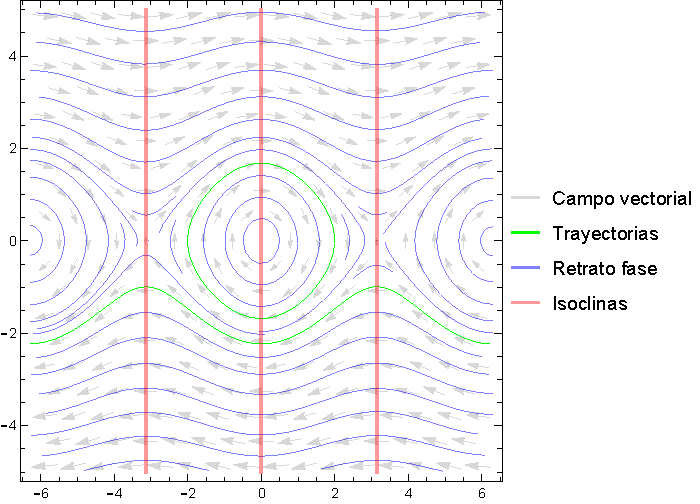
\includegraphics[width=0.7\textwidth]{img/Example.pdf}
	\caption{Campo vectorial, trayectorias, retrato fase e isoclinas ($c=0$) del sistema \eqref{eq: sisAut} asociado a $f(x,y)=(x,\sin{y})$.}
	\label{fig: example}
\end{figure}

Otro caso relevante para nuestro estudio, es dado cuando en el sistema autónomo bidimensional \eqref{eq: sisAutBid}, las funciones $f_1$ y $f_2$ son funciones polinómicas que denotaremos por $P(x,y)$ y $Q(x,y)$, respectivamente. A este tipo de sistemas se les denomina \emph{sistemas diferenciales polinómicos} de grado $n$, donde $n$ representa el grado máximo de los polinomios que componen el sistema. Usualmente, se asocian a un campo vectorial $X = P(x,y) \dfrac{\partial}{\partial x} + Q(x,y) \dfrac{\partial}{\partial y}$, con $P,Q \in C^r(U)$, donde, $U \subset \R^2$ es un abierto; una notación simplificada es $X = (P,Q)$. No existe distinción entre el campo vectorial $X$ y el sistema polinómico, ya que ambas representan formas equivalentes de denotación. \\

En algunas ocasiones las trayectorias o curvas solución de un sistema pueden ser cerradas y aisladas, es decir, no hay más trayectorias cerradas en una cierta región, dichas curvas solución son denominadas un \textit{ciclo límite}; si todas las trayectorias vecinas se acercan al ciclo límite decimos que el ciclo límite es \textit{estable} o \textit{atractor}, en otros casos el ciclo límite es \textit{inestable} o en casos excepcionales \textit{medio-estable}, donde las trayectorias vecinas se alejan y se acercan simultáneamente dentro y fuera del ciclo límite. En la \autoref{fig: CicloLimiteEstableInestable} se muestra un ejemplo de estos dos primeros casos.

\begin{figure}[H]
	\centering
	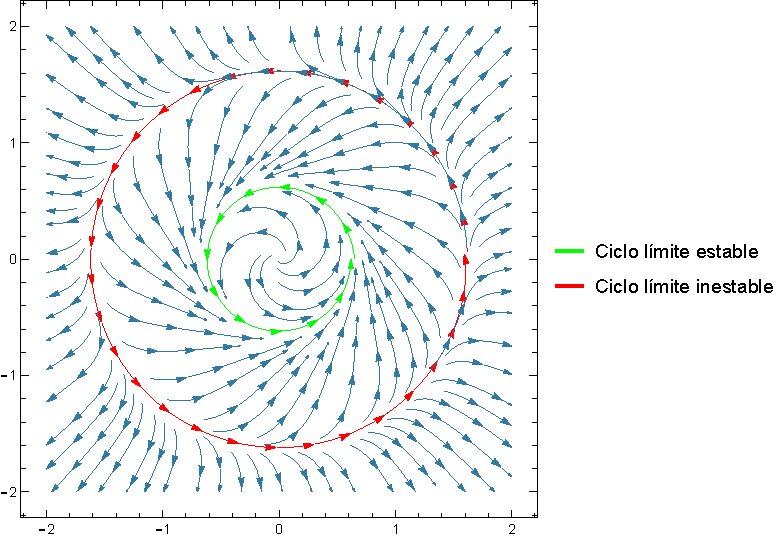
\includegraphics[width=0.7\textwidth]{img/CicloLimEstInest.pdf}
	\caption{Ciclos límite del sistema \eqref{eq: sisAut} asociado a \linebreak $f(x, y) = (-y + x(r^{4} -3r^{2} + 1), x + y(r^{4} -3r^{2} + 1))$ con $r^{2} = x^{2} + y^{2}$.}
	\label{fig: CicloLimiteEstableInestable}
\end{figure}

\begin{defi}
	Sea $\mathcal{M}_{n}(\R)$ el conjunto de matrices cuadradas de tamaño $n$ con entradas en $\R$ y sea $A \in \mathcal{M}_{n}(\R)$. Un escalar $\lambda \in \R$ es un valor propio de $A$ si existe un vector no nulo $v \in \Rn$ tal que, $Av = \lambda v$. Un vector no nulo $v \in \Rn$ tal que $Av = \lambda v$ es llamado un vector propio de $A$ asociado al valor propio $\lambda$.
\end{defi}

\begin{defi}
	Sea $A \in \mathcal{M}_{n}(\R)$ decimos que $A$ es diagonalizable si existe una matriz invertible $P \in \mathcal{M}_{n}(\R)$ y una matriz diagonal $D \in \mathcal{M}_{n}(\R)$ tal que $P^{-1}AP = D$.
\end{defi}

\begin{defi}
	Un punto $x_{0} \in \Rn$ es llamada una singularidad, punto de equilibrio o punto crítico de \eqref{eq: sisAut} si $f(x_{0})=0$. Un punto crítico $x_{0}$ es llamado un punto crítico hiperbólico de \eqref{eq: sisAut} si ninguno de los valores propios de la matriz jacobiana $Df(x_{0})$ tiene parte real cero, en caso contrario, se dice que $x_0$ es un punto crítico no hiperbólico. El sistema lineal \eqref{eq: sisLinAuto} con la matriz $A = Df(x_{0})$ es llamado la linealización de \eqref{eq: sisAut} en el punto $x_{0}$.
\end{defi}

\begin{defi}
	Un punto crítico $x_{0} \in \Rn$ es llamado un sumidero de \eqref{eq: sisAut} si todos los valores propios de la matriz jacobiana $Df(x_{0})$ tienen parte real negativa; es llamado una fuente de \eqref{eq: sisAut} si todos los valores propios de la matriz $Df(x_{0})$ tienen parte real positiva; y es llamado un punto silla de \eqref{eq: sisAut} si es un punto crítico hiperbólico y $Df(x_{0})$ tiene al menos un valor propio con parte real positiva y al menos un valor propio con parte real negativa.
\end{defi}

\begin{figure}[H]
	\centering
	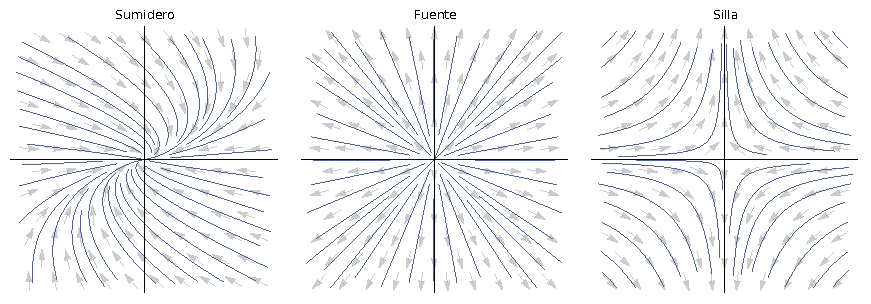
\includegraphics[width=1\textwidth]{img/EquilibriumPoints.pdf}
	\caption{Puntos críticos en el origen de sistemas lineales bidimensionales.}
	\label{fig: EquilibriumPoints}
\end{figure}

\begin{defi}
	Sean $E$ un subconjunto de $\Rn$, $f \in C^{1}(E)$ y $\phi_{t}$ el flujo del sistema \eqref{eq: sisAut} definida para todo $t \in \R$. Entonces un conjunto $S \subset E$ es llamado invariante con respecto al flujo $\phi_{t}$ si $\phi_{t} \subset S$ para todo $t\in \R$, y $S$ es llamado invariante positivo (o negativo) con respecto al flujo $\phi_{t}$ si $\phi_{t} \subset S$ para todo $t \geq 0$ (o $t\leq0$). Si además, $S$ es un conjunto conexo y cerrado, decimos que $S$ es una región de atrapamiento o ``trapping region" \cite[p. 204]{strogatz2014}.
\end{defi}

\begin{teo}[Poincaré-Bendixson]\label{teo: poincareB}
	Suponga que:
	\begin{enumerate}
		\item $R$ es un subconjunto cerrado y acotado en el plano;
		\item $\dot{x} = f(x)$ es un campo vectorial continuamente diferenciable en un conjunto abierto contenido en $R$;
		\item $R$ no contiene puntos de equilibrio; y
		\item Existe una trayectoria $C$ ``confinada'' en $R$, esto en el sentido de que inicia en $R$ y se mantiene en $R$ para todo tiempo futuro. 
	\end{enumerate}
	Entonces $C$ es una órbita cerrada, o una espiral que se acerca hacia una órbita cerrada cuando $t \rightarrow \infty$. En todo caso, R contiene una órbita cerrada.
\end{teo}

\begin{defi}
	Sea $x_{0}$ un punto crítico del sistema \eqref{eq: sisAut} definimos las variedades locales estable e inestable de $x_{0}$, $W^{s}(x_{0})$, $W^{u}(x_{0})$ como sigue
	\begin{equation*}
		\begin{aligned}
			W^{s}(x_{0}) &= \{ x\in U | \phi_{t}(x) \rightarrow x_{0} \text{ cuando } t\rightarrow \infty, \text{y } \phi_{t}(x)\in U \text{ para todo } t\geq 0 \}, \\
			W^{u}(x_{0}) &= \{ x\in U | \phi_{t}(x) \rightarrow x_{0} \text{ cuando } t\rightarrow -\infty, \text{y } \phi_{t}(x)\in U \text{ para todo } t \leq 0 \},
		\end{aligned}
	\end{equation*}
	donde $U \subseteq \Rn$ es una vecindad del punto crítico $x_{0}$. Si $U = \Rn$ los conjuntos $W^{s}(x_{0})$ y $W^{u}(x_{0})$ son llamados las variedades globales estable e inestable, respectivamente, del punto crítico $x_{0}$. 
\end{defi}

En ocasiones puede ocurrir que ciertas orbitas inician en la variedad inestable de un punto crítico $x_{0}$ y finalizan en la variedad estable de otro punto crítico $x_{1}$. Tales trayectorias son llamadas \textit{órbitas heteroclínicas} si $x_{0} \neq x_{1}$ y \textit{órbitas homoclínicas} si $x_{0} = x_{1}$. \\

Algo también de relevancia que se puede observar en la \autoref{fig:comparacion}, es que las trayectorias resaltadas dividen el plano de fases en regiones con diferentes comportamientos cualitativos, por ejemplo, la órbita homoclínica de la \linebreak \autoref{fig: homoclinic} divide el plano de fase en dos regiones: una con un comportamiento hiperbólico y la otra con una dinámica periódica alrededor del punto $(0,1)$. Dichas trayectorias con esta cualidad son denominadas \textit{separatrices}.

\begin{figure}[H]
	\centering
	\begin{subfigure}{0.49\textwidth}
		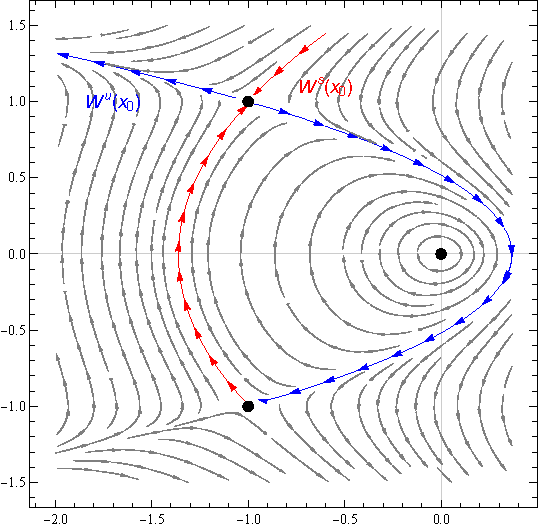
\includegraphics[width=\textwidth]{img/Heteroclinic.pdf}
		\caption{Retrato fase del sistema \eqref{eq: sisAut} asociado a $f(x,y) = (y-y^3, -x-y^2)$.}
		\label{fig: heteroclinic}
	\end{subfigure}
	\hfill
	\begin{subfigure}{0.49\textwidth}
		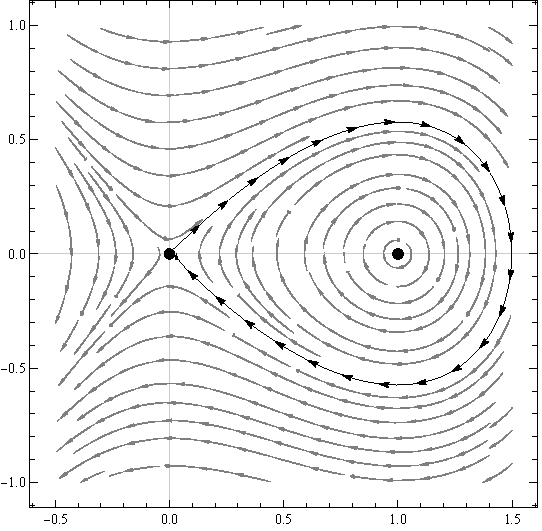
\includegraphics[width=\textwidth]{img/Homoclinic.pdf}
		\caption{Retrato fase del sistema \eqref{eq: sisAut} asociado a $f(x,y) = (y, x-x^2)$.}
		\label{fig: homoclinic}
	\end{subfigure}
	\caption{Variedad estable e inestable, órbitas heroclínicas y órbita homoclínica.}
	\label{fig:comparacion}
\end{figure}

\begin{teo}[Hartman-Grobman]\label{teo: hartman}
	Sea $E$ un subconjunto abierto de $\Rn$ que contiene al origen, sea $f \in C^{1}(E)$, y sea $\phi_{t}$ el flujo del sistema no lineal \eqref{eq: sisAut}. Suponga que $0$ es un punto crítico hiperbólico. Entonces existe un homeomorfismo $H$ de un conjunto abierto $U$ que contiene al origen hacia un conjunto abierto $V$ que contiene al origen, tal que para cada $x_{0} \in U$, existe un intervalo abierto $I_{0} \subset \R$ que contiene al cero, tal que para todo $x_{0} \in U$ y $t \in I_{0}$
	
	\begin{equation*}
		H \circ \phi_{t}(x_{0}) = e^{At}H(x_{0});
	\end{equation*}
	
	\noindent es decir, H mapea trayectorias de \eqref{eq: sisAut} que estan cerca del origen, hacia trayectorias de \eqref{eq: sisLinAuto} cerca al origen preservando la parametrización por tiempo.
\end{teo}

\noindent Este importante teorema nos indica que el retrato fase cerca a un punto crítico hiperbólico es topológicamente equivalente al retrato fase de la linealización en dicho punto de equilibrio. Aquí, la \textit{equivalencia topológica} es dada principalmente por la existencia de un \textit{homeomorfismo} (una deformación continua con inversa continua) que mapea trayectorias de un retrato fase local hacia el otro, preservando el sentido del tiempo (o la orientación de las trayectorias), lo cual es posible saberlo a través del determinante de la matriz jacobiana del homeomorfismo, si este es estrictamente positivo, decimos que la transformación preserva el sentido del tiempo o, en caso contrario (determinante negativo), la orientación se revierte. Intuitivamente, dos retratos fases son topológicamente equivalentes si una es una versión distorsionada de la otra. A modo de ejemplo, considere la \autoref{fig: exampleHartman}. \\

\begin{figure}[H]
	\centering
	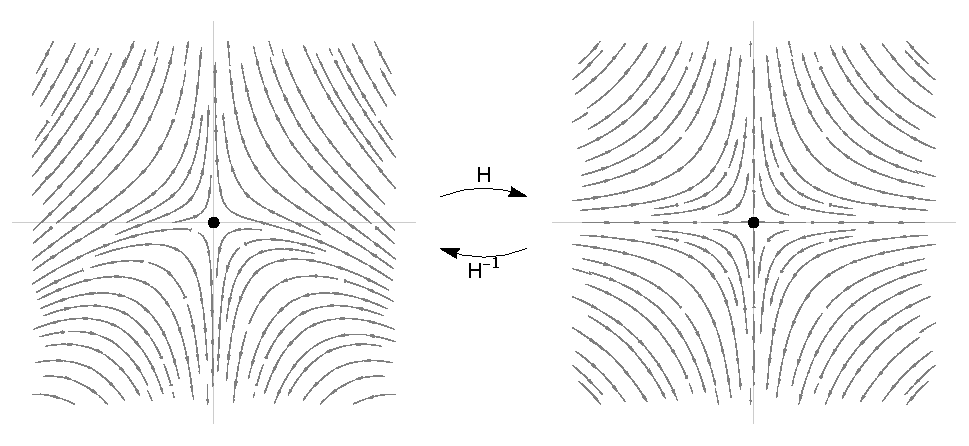
\includegraphics[width=1\textwidth]{img/exampleHartman.pdf}
	\caption{Retrato fase del sistema \eqref{eq: sisAut} asociado a $f(x,y) = (-x, y+x^2)$ y su respectiva transformación en el origen dada por el homeomorfismo $H(x,y)=(x,x+\dfrac{y^{2}}{3})$}
	\label{fig: exampleHartman}
\end{figure}

Dada la posibilidad de que existan puntos críticos no hiperbólicos en el sistema \eqref{eq: sisAut}, es decir, puntos $x_{0}$ donde alguno de los valores propios de la matriz jacobiana $Df(x_0)$ posee parte real nula, resulta de interés analizar el comportamiento dinámico local en dichos puntos. En estas singularidades no es posible aplicar directamente el \Cref{teo: hartman}, aunque el Teorema de la variedad central nos permita analizar el comportamiento local en los puntos críticos no hiperbólicos donde su matriz jacobiana no se anule (puntos críticos no degenerados), es de nuestro interés analizar el comportamiento de las singularidades que no cumplan esta ultima condición, por lo que se procede a realizar un cambio de coordenadas con el objetivo de eliminar la singularidad y, de esta manera, poder estudiar el comportamiento cualitativo en su entorno mediante uno de estos teoremas. A este procedimiento se le denomina \textit{desingularización del campo vectorial} \eqref{eq: sisAut}. Existen diversas técnicas para desingularizar un sistema dinámico, sin embargo, en este trabajo se enfocará en la desingularización a través del \textit{método de blowing-up} o \textit{blow-up}.

\subsection*{Blow-up en $ \R^2$}
\addcontentsline{toc}{subsection}{Blow-up en $ \R^2$}
En la teoría cualitativa de los sistemas dinámicos, especialmente para sistemas planos, el blow-up es una herramienta fundamental basada en cambios de variables utilizada para estudiar singularidades. Su objetivo es simplificar el estudio de un punto crítico complicado (generalmente en el origen) transformándolo en un círculo que contiene un número finito de nuevos puntos criticos, a menudo hiperbólicos. \\

Sea 0 un punto de equilibrio de un campo vectorial suave $X \in C^{\infty}(\R^{2})$. Considere la función
\begin{equation}
	\begin{aligned}
		\psi : \mathbb{S}^{1} \times \mathbb{R} &\longrightarrow \R^{2} \\
		(\theta , r) &\longmapsto (r \, \cos{\theta}, r \, \sin{\theta}),
	\end{aligned}
\end{equation}
donde $\mathbb{S}^{1}$ representa la circunferencia unitaria centrada en el origen.
Podemos definir un campo vectorial suave, $\tilde{X}$ en el cilindro $\mathbb{S}^{1} \times \mathbb{R}$ tal que la aplicacion lineal $\psi_{*}:T_{p}M \longrightarrow T_{\psi(p)}M$ envia el campo vectorial $\tilde{X}$ a $X$, es decir, $\psi_{*}(\tilde{X})=X$, en el sentido que, $D\psi_{v}(\tilde{X}(v)) = X(\psi(v))$. Esto se llama el retroceso (pull back) de $X$ por $\psi$. No es nada más que $X$ escrito en coordenadas polares. La aplicación $\psi$ es un difeomorfismo suave, por lo tanto, un cambio de coordenadas suave en $\mathbb{S}^{1} \times (0,\infty)$, pero no en $\{r=0\}$; aquí, $\psi$ envía $\{r=0\}$ a $(0,0)$, y como tal, la aplicación inversa $\psi^{-1}$ ``explota'' el origen a un círculo. Para estudiar el retrato de fases de $X$ en un vecindario $V$ del origen, basta claramente estudiar el retrato de fases de $\tilde{X}$ en el vecindario $\psi^{-1}(V)$ del círculo $\mathbb{S}^{1}\times \{0\}$. Básicamente, este método se basa en convertir el sistema a coordenadas polares y estudiarlo en $r=0$, en caso de que el campo vectorial se anule, consideramos el nuevo campo vectorial $$\bar{X}=\dfrac{1}{r^{k}}\tilde{X},$$ donde $k$ es el menor natural que no permite esta nulidad; este cociente no cambia las órbitas de $\tilde{X}$ ni su sentido de dirección, sino la parametrización por tiempo $t$. \\

%Aunque el cilindro es una buena superficie para obtener una visión global de $\tilde{X}$ y su retrato de fases, a menudo es menos apropiado para hacer cálculos, ya que constantemente tenemos que tratar con expresiones trigonométricas. Por esa razón puede ser preferible hacer los cálculos en diferentes cartas.
%
%En las partes del cilindro dadas, respectivamente, por $\theta\in(-\pi/2,\pi/2)$ y $\theta\in(\pi/2,3\pi/2)$ usamos una carta dada por
%$$
%K^{x}:(\theta,r)\mapsto (r\cos\theta,\tan\theta)=(\bar{x},\bar{y}).
%$$
%
%En esta carta la expresión del blow-up $\psi$ está dada por
%$$
%\psi^{x}:(\bar{x},\bar{y})\mapsto (\bar{x},\bar{x}\bar{y}).
%$$
%
%En efecto vemos que
%$$
%\psi=\psi^{x}\circ K^{x}:(\theta,r)\xmapsto{K^{x}}(r\cos\theta,\tan\theta)
%\xmapsto{\psi^{x}}(r\cos\theta,r\cos\theta\tan\theta)=(r\cos\theta,r\sin\theta).
%$$
%
%Llamamos a esto un \textit{blow-up en la dirección $x$}; el retroceso de $X$ mediante $\psi^{x}$ se denota por $\tilde{X}^{x}$, es decir $(\psi^{x})_{*}(\tilde{X}^{x})=X$.
%
%En las partes del cilindro dadas, respectivamente, por $\theta\in(0,\pi)$ y $\theta\in(\pi,2\pi)$ usamos una carta dada por
%$$
%K^{y}:(\theta,r)\mapsto (\cot\theta,r\sin\theta)=(\bar{x},\bar{y}).
%$$
%
%En esta carta la expresión del blow-up $\psi$ está dada por
%$$
%\psi^{y}:(\bar{x},\bar{y})\mapsto (\bar{x}\bar{y},\bar{y}).
%$$
%
%en el sentido de que $\psi=\psi^{y}\circ K^{y}$. Llamamos a esto un \textit{blow-up en la dirección $y$}; el retroceso de $X$ mediante $\psi^{y}$ se denota por $\tilde{X}^{y}$, es decir $(\psi^{y})_{*}(\tilde{X}^{y})=X$. Tanto $\psi^{x}$ como $\psi^{y}$ se llaman \textit{blow-ups direccionales}.

Como se mencionó anteriormente, al aplicar el blow-up al origen, este se transforma en un conjunto que puede contener nuevos puntos de equilibrio. Si alguno de estos puntos no resulta ser hiperbolico, es posible iterar nuevamente el proceso hasta que se logre lo ideal. De este modo, tras un número finito de blow-ups sucesivos, se puede determinar el retrato de fase local asociado a la singularidad original.

%\subsection{Compactificación de Poincaré}
%Al investigar la estructura cualitativa del retrato de fase de sistemas de ecuaciones diferenciales ordinarias (EDOs) definidos en todo el plano, resulta especialmente relevante comprender el comportamiento de las trayectorias a medida que las variables $x$ e $y$ tienden a infinito, es decir, su comportamiento ``en el infinito''.
%
%Por ejemplo, estudiar lo que ocurre en el infinito puede permitir identificar con claridad el estado de equilibrio al que se dirige una separatriz que parte de un punto de silla, o bien establecer la existencia de un ciclo límite. En consecuencia, el análisis del comportamiento de las trayectorias en el infinito constituye un aspecto fundamental en el estudio cualitativo de sistemas dinámicos.
%
%Una forma de obtener información sobre el comportamiento de tales trayectorias es (intentar) compactificar el espacio cartesiano, de modo que el campo vectorial se extienda a una esfera unitaria $\mathbb{S}^{2}$ que contenga los ``puntos en el infinito''; este método es atribuido a Poincaré y es conocido como la \textit{compactificación de Poincaré}.
%
%Consideremos el campo vectorial plano dado por
%\begin{equation}
%	\begin{aligned}
%		\dot{x} &= f(x, y) \\
%		\dot{y} &= g(x, y),
%	\end{aligned}
%	\label{eq: camVecPlano}
%\end{equation}
%la esfera unitaria $\mathbb{S}^{2} = \{ (x,y,z) : x^{2} + y^{2} + z^{2} = 1 \}$ y el plano tangente $\Pi$ al polo norte; que es el punto con coordenadas (0,0,1). El traslado del sistema \eqref{eq: camVecPlano} al plano $\Pi$, dada por la función natural $(x,y) \longmapsto (x,y,1)$ es:
%\begin{equation}
%	\begin{aligned}
%		\dot{x} &= f(x, y) \\
%		\dot{y} &= g(x, y) \\
%		\dot{z} &= 0
%	\end{aligned}
%	\label{eq: 3camVec}
%\end{equation}
%La idea es ``proyectar'' el sistema \eqref{eq: camVecPlano} a la esfera unitaria mediante una proyección central; entonces, el comportamiento del sistema cerca del infinito es el mismo que el comportamiento del sistema proyectado cerca del ecuador de la esfera.
%
%La proyección central se define de la siguiente manera: Un punto $p \in \Pi$ se asigna a la esfera asignando el único punto en la esfera que se encuentra en el segmento de línea desde el origen en $\R ^{3}$ hasta el punto $p$ (Veáse la \autoref{fig: poincareCompactification}). Para evitar un campo vectorial especificado por tres componentes, estudiaremos el campo vectorial proyectado restringido a un sistema de coordenadas en la esfera donde el campo vectorial es nuevamente plano. Además, para obtener la compactificación deseada, elegiremos coordenadas locales definidas en conjuntos abiertos que contienen porciones del ecuador de la esfera.
%
%La proyección central $Q: \Pi \rightarrow \mathbb{S}^{2}$ es dada por:
%\begin{equation*}
%	Q(x,y,1)=(X,Y,Z)=(\dfrac{x}{\sqrt{x^{2}+y^{2}+1}},\dfrac{y}{\sqrt{x^{2}+y^{2}+1}},\dfrac{1}{\sqrt{x^{2}+y^{2}+1}}).
%\end{equation*}
%
%\begin{figure}
%	\centering
%	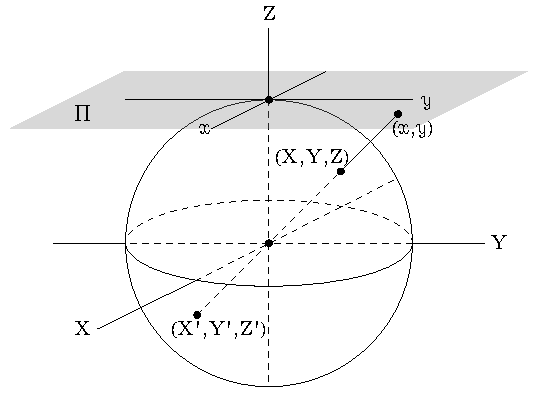
\includegraphics[width=0.7\textwidth]{img/poincareCompactification.pdf}
%	\caption{Esfera de Poincaré.}
%	\label{fig: poincareCompactification}
%\end{figure}

\section{Bifurcaciones}

Si
\begin{equation}
	\dot{x} = f_{\mu}(x), \quad x \in \Rn, \quad \mu \in \R^{k},
	\label{eq: sisParametro}
\end{equation}
es un sistema de ecuaciones diferenciales que depende del parámetro $k$-dimensional $\mu$, entonces los puntos de equilibrio de \eqref{eq: sisParametro} son dados por las soluciones de la ecuación $f_{\mu}(x) = 0$. Cuando $\mu$ varia, la estructura cualitativa del flujo puede cambiar, en particular, puntos críticos pueden ser creados o destruidos, o también su estabilidad puede cambiar, de igual manera trayectorias cerradas pueden aparecer o desaparecer. Estos cambios cualitativos en las dinámicas del sistema son llamadas \textit{bifurcaciones} y los valores paramétricos para los cuales este cambio ocurre son llamados \textit{valores de bifurcación}. Dependiendo del comportamiento del sistema al manipular dichos parámetros surgen diversos tipos de bifurcación. Sin perdida de generalidad vamos a suponer que en cada un de los tipos de bifurcación que veremos a continuación el valor de bifurcación es $\mu=0$.

\subsection{Bifurcación silla-nodo}

La bifurcación silla-nodo es el mecanismo básico en el cual puntos de equilibrio son creados y destruidos dependiendo de los parametros usados en el sistema \ref{eq: sisParametro}. En la \autoref{fig: bifSillaNodo} se ejemplifica este tipo de bifurcación, en el cual para $\mu<0$ no existe ningún punto crítico, para $\mu=0$ existe un único punto crítico y para $\mu>0$ hay presencia de dos puntos críticos.

\begin{figure}[H]
	\centering
	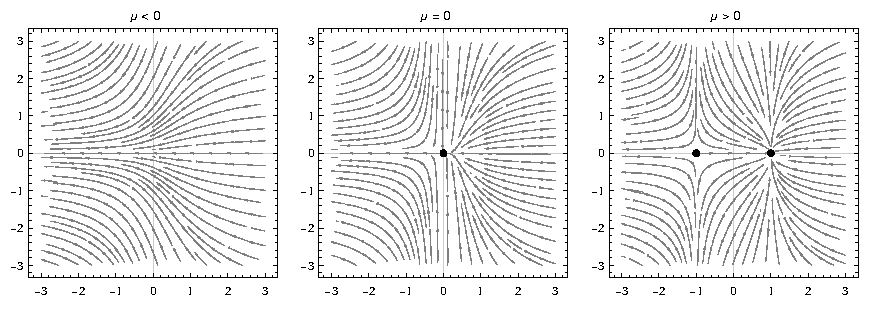
\includegraphics[width=1\textwidth]{img/bifSillaNodo.pdf}
	\caption{Bifurcación silla-nodo en el sistema \eqref{eq: sisParametro} asociado a $f_{\mu}(x,y)=(\mu - x^2,-y)$.}
	\label{fig: bifSillaNodo}
\end{figure}

\subsection{Bifurcación transcrítica}

Existen ciertas situaciones científicas en las que debe existir un punto crítico para todos los valores de un parámetro y nunca puede destruirse. Por ejemplo, en ecuaciones logísticas y otros modelos simples para el crecimiento de una sola especie, existe un punto crítico en la población cero, independientemente del valor de la tasa de crecimiento. Sin embargo, dicho punto crítico puede cambiar su estabilidad al variar el parámetro. La bifurcación transcrítica es el mecanismo estándar para tales cambios de estabilidad. En la \autoref{fig: bifTranscritica} se ejemplifica este tipo de bifurcación, en donde el origen para $\mu<0$ es un nodo atractor, un punto silla-nodo para el valor de bifurcación, y una silla hiperbólica para $\mu>0$.

\begin{figure}[H]
	\centering
	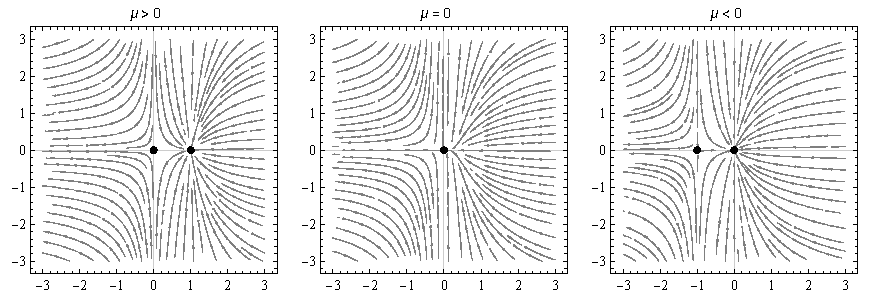
\includegraphics[width=1\textwidth]{img/bifTranscritica.pdf}
	\caption{Bifurcación transcrítica en el sistema \eqref{eq: sisParametro} asociado a $f_{\mu}(x,y)=(\mu x - x^2,-y)$.}
	\label{fig: bifTranscritica}
\end{figure}

\subsection{Bifurcaciones de Pitchfork}

Pasamos ahora a un tercer tipo de bifurcación, la llamada bifurcación de Pitchfork o bifurcación en horquilla. Esta bifurcación es común en problemas físicos con simetría. Por ejemplo, muchos problemas presentan simetría espacial entre la izquierda y la derecha. En tales casos, los puntos críticos tienden a aparecer y desaparecer en pares simétricos. Existen dos tipos muy diferentes de bifurcación en horquilla.

\subsubsection{Bifurcación de Pitchfork supercrítica}

Este tipo de bifurcación es característico de sistemas que son invariantes ante el cambio de variables $x \rightarrow -x$. Por ejemplo, consideremos el sistema 
\begin{equation*}
	\left\{
	\begin{aligned}
		\dot{x} &= \mu x +x^3, \\
		\dot{y} &= -y,
	\end{aligned}
	\right.
\end{equation*}
si en la primera ecuación reemplazamos $x$ por $-x$ tenemos
\begin{equation*}
	\begin{aligned}
		\dot{(-x)} &= \mu (-x) +(-x)^3 \\
		-\dot{x} &= -(\mu x+x^3) \\
		\dot{x} &= \mu x +x^3
	\end{aligned}
\end{equation*}
Por tanto obtenemos el sistema original. Esta invariancia es la expresión matemática de la simetría izquierda-derecha mencionada anteriormente. El retrato fase de este sistema para diferentes valores de $\mu$ se puede visualizar en la \autoref{fig: bifPitchforkSup}, en donde dos puntos críticos aparacen en pares simétricos para $\mu>0$.

\begin{figure}[H]
	\centering
	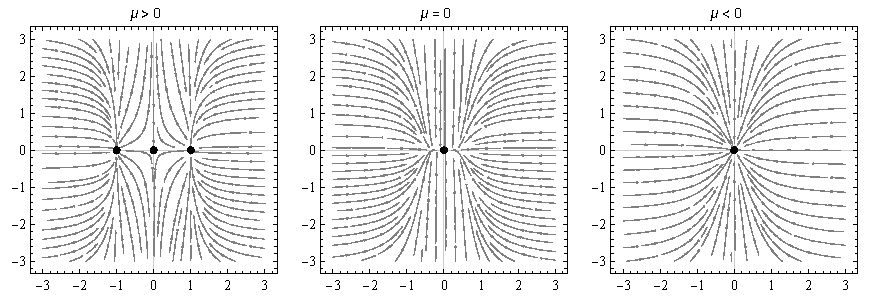
\includegraphics[width=1\textwidth]{img/bifPitchforkSup.pdf}
	\caption{Bifurcación de Pitchfork supercrítica en el sistema \eqref{eq: sisParametro} asociado a $f_{\mu}(x,y)=(\mu x - x^3,-y)$.}
	\label{fig: bifPitchforkSup}
\end{figure}

\subsubsection{Bifurcación de Pitchfork subcrítica}

De manera similar que en el supercrítico ahora los puntos críticos solo existen por debajo del valor de bifurcación ($\mu < 0$) como se muestra en la \autoref{fig: bifPitchforkSub}.

\begin{figure}[H]
	\centering
	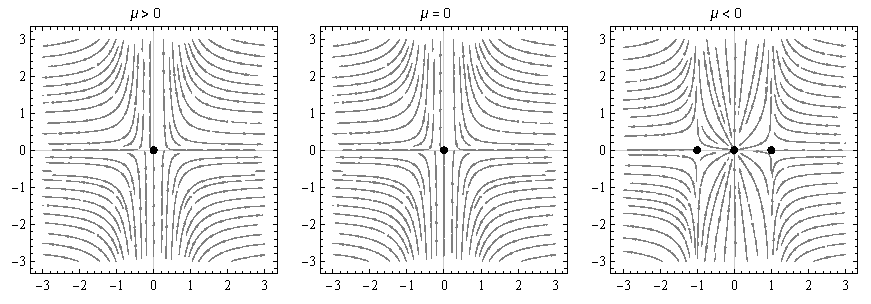
\includegraphics[width=1\textwidth]{img/bifPitchforkSub.pdf}
	\caption{Bifurcación de Pitchfork subcrítica en el sistema \eqref{eq: sisParametro} asociado a $f_{\mu}(x,y)=(\mu x + x^3,-y)$.}
	\label{fig: bifPitchforkSub}
\end{figure}

\subsection{Bifurcaciones de Hopf}

Supongamos que un sistema bidimensional tiene un punto crítico estable, el cual, existe para cualquier valor paramétrico. ¿Cuáles son las posibles maneras en que podría perder estabilidad al variar un parámetro $\mu$? Los autovalores del Jacobiano son la clave. Si el punto crítico es estable, los autovalores $\lambda _{1}$, $\lambda _{2}$ en el plano complejo, deben estar en el semiplano izquierdo Re$\lambda <0$. Dado que las $\lambda$'s satisfacen una ecuación cuadrática con coeficientes reales, existen dos posibles escenarios: o bien los autovalores son reales y negativos o bien son conjugados complejos. Para desestabilizar el punto crítico, necesitamos que uno o ambos autovalores crucen al semiplano derecho al variar $\mu$, analíticamente, este hecho se ve reflejado de la siguiente manera: considere los valores propios complejos del jacobiano como $\lambda(\mu)=\alpha(\mu) \pm i\omega(\mu)$. En el valor de bifurcación $\mu=\mu_0$ el jacobiano debe poseer valores propios complejos puros, es decir, $\alpha(\mu_0)=0$ y $\omega(\mu_0)>0$, conocida como \textit{condición espectral}; ahora, el hecho de que uno o ambos autovalores crucen al semiplano derecho al variar $\mu$, se describe mediante la \textit{condición de transversalidad} $$\left. \dfrac{d}{d\mu}(\alpha(\mu)) \right|_{\mu=\mu_0} \neq 0.$$ Además, el \textit{primer coeficiente de Lyapunov} ($l_1$) no debe anularse, este coeficiente será especificado más adelante, bajo estas condiciones decimos que ocurre una \textit{bifurcación de Hopf} en $\mu=\mu_0$. Dado el caso de que $l_1 = 0$, y la aplicación $\mu \mapsto (\alpha(\mu), l_1(\mu))$, sea regular en $\mu=\mu_0$, en el sentido que
\begin{equation*}
	\det \left. \begin{pmatrix}
		\dfrac{\partial \alpha(\mu)}{\partial A} & \dfrac{\partial \alpha(\mu)}{\partial B} \\[6pt]
		\dfrac{\partial l_1(\mu)}{\partial A} & \dfrac{\partial l_1(\mu)}{\partial B} 
	\end{pmatrix} \right|_{\mu=\mu_0} \neq 0,
\end{equation*}
y si además, el \textit{segundo coeficiente de Lyapunov} ($l_2$) no se anula, este coeficiente será especificado más adelante; decimos que ocurre una \textit{bifurcación de Hopf generalizada o de Bautin}. Pese a lo anteriormente descrito las bifurcaciones de Hopf ocurren en espacios de fases de cualquier dimensión $n \geq 2$.
Al igual que las bifurcaciones en horquilla, las bifurcaciones de Hopf se presentan en variedades supercríticas y subcríticas.

\subsubsection{Bifurcación de Hopf supercrítica}

En términos del flujo en el espacio de fases, una bifurcación de Hopf supercrítica ocurre cuando una espiral estable se transforma en una espiral inestable rodeada por un pequeño ciclo límite estable casi elíptico, o de igual manera cuando $l_1 > 0$. La ejemplificación de este tipo de bifurcación se puede evidenciar en la \autoref{fig: bifHopfSup}, donde un ciclo límite estable aparece para $\mu>0$, con el origen perdiendo su estabilidad en este caso.

\begin{figure}[H]
	\centering
	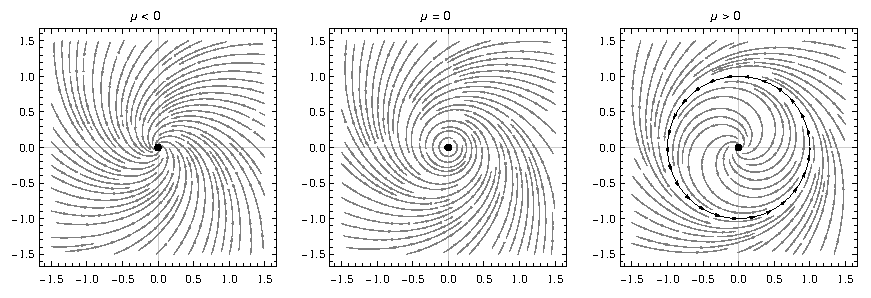
\includegraphics[width=.99\textwidth]{img/bifHopfSup.pdf}
	\caption{Bifurcación de Hopf supercrítica en el sistema \eqref{eq: sisParametro} asociado a $f_{\mu}(r,\theta)=(\mu r - r^3,1 + r^2)$.}
	\label{fig: bifHopfSup}
\end{figure}

\subsubsection{Bifurcación de Hopf subcrítica}

El caso subcrítico es siempre mucho más dramático y potencialmente peligroso en aplicaciones de ingeniería. Ocurre cuando $l_1 < 0$, tras la bifurcación, las trayectorias deben saltar a un atractor distante, que puede ser un punto fijo, otro ciclo límite (inestable), el infinito o, en tres dimensiones o más, un atractor caótico.

\begin{figure}[H]
	\centering
	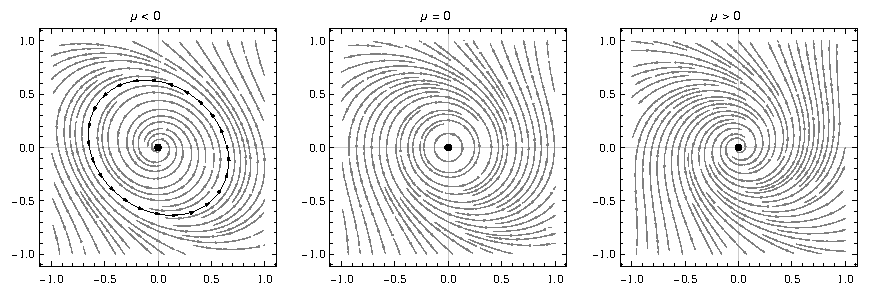
\includegraphics[width=.99\textwidth]{img/bifHopfSub.pdf}
	\caption{Bifurcación de Hopf subcrítica en el sistema \eqref{eq: sisParametro} asociado a $f_{\mu}(x,y)=(\mu x-y+x y^2, x+a y+y^3)$.}
	\label{fig: bifHopfSub}
\end{figure}

\section{Modelos ecológicos}
 
Dentro de la biología matemática, los modelos ecológicos desempeñan un papel fundamental para predecir el comportamiento de diversas poblaciones, ya sean de bacterias, plantas, animales, etc. Existen múltiples tipos de modelos ecológicos, los cuales dependen de diversos factores, como el \textit{crecimiento poblacional}. Este crecimiento puede manifestarse de diferentes formas: una población $P(t)$, donde $t$ representa el tiempo, puede experimentar distintos tipos de crecimiento, siendo los más comunes el crecimiento exponencial y el crecimiento logístico.

\noindent Los modelos basados en crecimiento exponencial resultan poco realistas a largo plazo, ya que no consideran limitaciones ambientales ni de recursos. Por ello, los modelos logísticos, en los que $P(t)$ presenta un crecimiento limitado y controlado por la capacidad del entorno, resultan más relevantes para el estudio de poblaciones reales. A estos modelos se les denomina \textit{ecuaciones logísticas}. 

\noindent Por ejemplo en los modelos presa-depredador, los efectos beneficiosos que la comida tiene sobre los depredadores individuales son evidentes. En general, cuanto más alimento consumen los depredadores, mayores son sus tasas de crecimiento, desarrollo y natalidad, y menores sus tasas de mortalidad. Esto, después de todo, es la base de la competencia intraespecífica: las altas densidades, que implican pequeñas cantidades de alimento por individuo, conducen a bajas tasas de crecimiento, altas tasas de mortalidad, etc. Sin embargo, existen diversas maneras en que las relaciones entre la tasa de consumo y el beneficio para el consumidor pueden ser más complejas de lo que parecen inicialmente. A estas relaciones se le denominan \textit{respuestas funcionales} y se dividen en varios tipos. Holling (1959) fue el primero en distinguir tres tipos de respuesta funcional.
\subsection{Respuesta funcional tipo 1}
La respuesta funcional más básica, la de tipo 1, es la que se asume por ejemplo en las ecuaciones de Lotka-Volterra: la tasa de consumo aumenta linealmente con la densidad de presas. Esto se indica mediante la constante $b$ en el sistema \ref{eq: lotka-volterra}.

\begin{figure}[H]
	\centering
	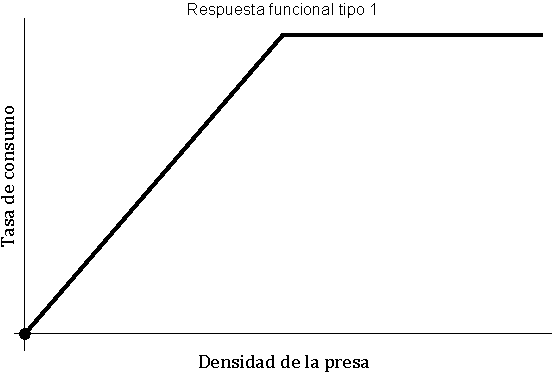
\includegraphics[width=.5\textwidth]{img/type1FunctionalResponse.pdf}
	\caption{Respuesta funcional de Holling tipo 1.}
	\label{fig: type1FunctionalResponse}
\end{figure}

\subsection{Respuesta funcional tipo 2}
La respuesta funcional observada con mayor frecuencia es la respuesta de tipo 2, en la que la tasa de consumo aumenta con la densidad de presas, pero se desacelera gradualmente hasta alcanzar una meseta en la que la tasa de consumo se mantiene constante independientemente de la densidad de presas.

\noindent La respuesta de tipo 2 se explica por el hecho de que un depredador debe dedicar tiempo a manipular cada presa que consume (es decir, perseguirla, dominarla y consumirla, y luego prepararse para la búsqueda). A medida que aumenta la densidad de presas, encontrarla se vuelve cada vez más fácil.

\noindent Sin embargo, manipular una presa sigue requiriendo el mismo tiempo, y por lo tanto, la manipulación en general ocupa una proporción cada vez mayor del tiempo del depredador, hasta que, a altas densidades de presas, este dedica prácticamente todo su tiempo a manipularla. Por lo tanto, la tasa de consumo se aproxima y luego alcanza un máximo (la meseta), determinado por el número máximo de manipulaciones que se pueden realizar en el tiempo total disponible.

\noindent Este comportamiento es descrito a través de la expresión $$\dfrac{A}{N+B},$$ donde $A$ y $B$ son constantes positivas y $N$ representa la población de las presas.

\begin{figure}[H]
	\centering
	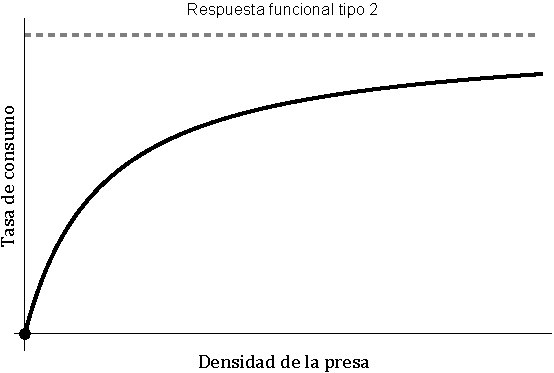
\includegraphics[width=.5\textwidth]{img/type2FunctionalResponse.pdf}
	\caption{Respuesta funcional de Holling tipo 2.}
	\label{fig: type2FunctionalResponse}
\end{figure}

\subsection{Respuesta funcional tipo 3}
Las respuestas funcionales de tipo 3, a altas densidades de presas, son similares a una respuesta de tipo 2, y las explicaciones para ambas son las mismas. Sin embargo, a bajas densidades de presas, la respuesta de tipo 3 presenta una fase de aceleración, donde un aumento de la densidad conduce a un aumento más que lineal de la tasa de consumo. Por lo tanto, en general, una respuesta de tipo 3 tiene forma de S o sigmoidea. 
En general, esta forma sigmoidea y la respuesta funcional de tipo 3 surgirán siempre que un aumento de la densidad de alimento conduzca a un aumento de la eficiencia de búsqueda o tasa de ataque del consumidor, o a una disminución de su tiempo de manipulación, ya que ambas determinan la tasa de consumo. Por ejemplo, un depredador puede interesarse por una especie de presa en particular solo cuando su abundancia relativa en la comunidad de presas es suficientemente alta.
Esta forma sigmoidea se representa a través de $$\dfrac{AN}{N^2+B^2},$$ donde $A$ y $B$ son constantes positivas y $N$ representa la población de las presas.

\begin{figure}[H]
	\centering
	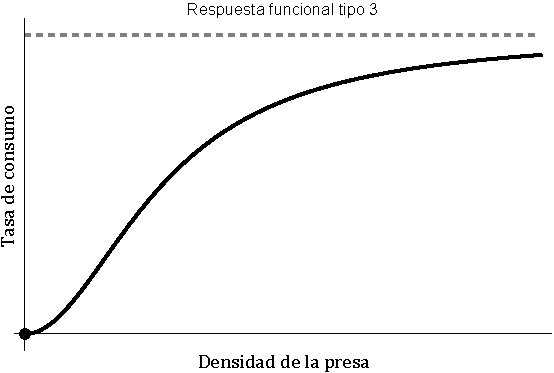
\includegraphics[width=.5\textwidth]{img/type3FunctionalResponse.pdf}
	\caption{Respuesta funcional de Holling tipo 3.}
	\label{fig: type3FunctionalResponse}
\end{figure}

%\subsection*{Respuesta funcional tipo 4}
%
%
%\begin{figure}[H]
%	\centering
%	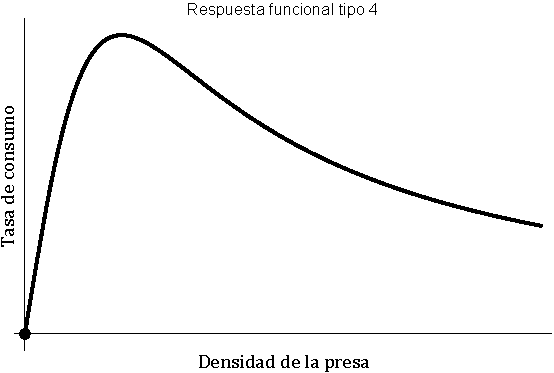
\includegraphics[width=.5\textwidth]{img/type4FunctionalResponse.pdf}
%	\caption{Respuesta funcional tipo 4.}
%	\label{fig: type4FunctionalResponse}
%\end{figure}
\newpage
\subsection{Modelo Lotka-Volterra}

Volterra (1926) fue el primero en proponer un modelo simple para la depredación de una especie por otra para explicar los niveles oscilatorios de ciertas capturas de peces en el Adriático. Si $N(t)$ es la población de presas y $P(t)$ la del depredador en el tiempo $t$, entonces el modelo de Volterra es

\begin{equation}
	\left\{
	\begin{aligned}
		\dfrac{dN}{dt} = N(a-bP), \\
		\dfrac{dP}{dt} = P(cN-d),
	\end{aligned}
	\right.
	\label{eq: lotka-volterra}
\end{equation}
donde $a,b,c$ y $d$ son constantes positivas que representan las interacciones entre la presa y el depredador, aquí: $a$ es la tasa de crecimiento de las presas, $b$ es la tasa de captura de los depredadores, $c$ es la tasa de conversión de presas capturadas en nuevos depredadores y $d$ es la tasa de mortalidad de los depredadores, dicho esto, los supuestos en este modelo son:
\begin{enumerate}
	\item La presa, en ausencia de depredación, crece ilimitadamente de forma maltusiana; este es el término $aN$.
	\item El efecto de la depredación es reducir la tasa de crecimiento per cápita de la presa en un término proporcional a las poblaciones de presas y depredadores; este es el término $-bNP$.
	\item La contribución de la presa a la tasa de crecimiento de los depredadores es $cNP$, es decir, es proporcional a las presas disponibles, así como al tamaño de la población de depredadores.
	\item En ausencia de presas para su sustento, la tasa de mortalidad del depredador resulta en una disminución exponencial; es decir, el término $-dP$.
\end{enumerate}
El modelo \eqref{eq: lotka-volterra} se conoce como el \textit{modelo de Lotka-Volterra}, ya que Lotka (1920) también derivó las mismas ecuaciones a partir de una reacción química hipotética que, según él, podría exhibir un comportamiento periódico en las concentraciones químicas. Aunque este modelo cuenta con ciertas desventajas como el hecho de que no considera la limitacón de recursos, es un punto de partida para modelos ecológicos más realistas.

\subsection{Modelo Leslie-Gower}

El modelo presa-depredador de Leslie-Gower es una variante del modelo de Lotka-Volterra. La principal diferencia radica en la incorporación de un término adicional que convierte el crecimiento exponencial de las presas, presente en el sistema de Lotka-Volterra, en un crecimiento logístico; además la capacidad de carga de los depredadores es directamente proporcional a la densidad de las presas. En este caso, se considera la capacidad de carga del entorno $K$, lo que limita el crecimiento de la población de presas. El modelo resultante es el siguiente:
\begin{equation}
	\left\{
	\begin{aligned}
		\dfrac{dN}{dt} &= N\left[r\left(1-\dfrac{N}{K}\right)-PR(N)\right], \\
		\dfrac{dP}{dt} &= k\left( 1 - \dfrac{hP}{N} \right),
	\end{aligned}
	\right.
	\label{eq: leslie}
\end{equation}
donde $r, \; k$ y $h$ son constantes positivas y $R(N)$ representa alguna de las respuestas funcionales descritas anteriormente. \\

Otra variante que se encuentra en diversas fuentes es aquella en la que se incorpora algún tipo de respuesta funcional a los depredadores:
\begin{equation}
	\left\{
	\begin{aligned}
		\dfrac{dN}{dt} &= N\left[r\left(1-\dfrac{N}{K}\right)-PR(N)\right], \\
		\dfrac{dP}{dt} &= -d+eR(N),
	\end{aligned}
	\right.
	\label{eq: leslie-gower}
\end{equation}
donde $d$ y $e$ representan constantes positivas.
	\chapter[Modelo de Leslie-Gower]{El modelo de Leslie-Gower con respuesta funcional sigmoidea}

En este capítulo se analiza el modelo presa-depredador de tipo Leslie-Gower propuesto por González-Olivares et al. (2015)\cite{articulo}, en el cual la población de presas exhibe una respuesta funcional de Holling tipo 3, caracterizada por su forma sigmoidea.

\section{Descripción del modelo}

El modelo se describe mediante el siguiente sistema autónomo de ecuaciones diferenciales ordinarias de tipo Kolmogorov:

\begin{equation}
	X_{\mu}:
	\begin{cases}
		\dfrac{dx}{dt} = \left(r \left(1 - \dfrac{x}{K}\right) - \dfrac{q x y}{x^2 + a^2}\right) x, \\
		\dfrac{dy}{dt} = s \left(1 - \dfrac{y}{n x}\right) y,
	\end{cases}
	\label{eq:modelo1}
\end{equation}

\noindent donde $x(t)$ y $y(t)$ representan las densidades poblacionales de presas y depredadores, respectivamente, para $t \geq 0$. Los parámetros $\mu = (r, a, s, K, n, q) \in \R^6_{+}$ son estrictamente positivos y tienen el siguiente significado biológico:

\begin{itemize}
	\item $r$: tasa de crecimiento intrínseco de las presas;
	\item $K$: capacidad de carga ambiental de las presas;
	\item $q$: tasa máxima de consumo per cápita de los depredadores (tasa de saciedad);
	\item $a$: cantidad de presas necesarias para alcanzar la mitad de $q$ (media de la tasa de saturación);
	\item $s$: tasa de crecimiento intrínseco de los depredadores;
	\item $n$: medida de la calidad alimenticia, que indica la eficiencia de conversión de presas consumidas en nuevos depredadores.
\end{itemize}

\noindent El sistema \eqref{eq:modelo1} no está definido en $x=0$ (eje $y$), por lo que el dominio biológicamente relevante es el conjunto $\Omega = \{ (x,y) \in \R^2 \mid x > 0, \; y \geq 0 \}$.

\section{Análisis}

Los puntos críticos de \eqref{eq:modelo1} se obtienen resolviendo el sistema

\begin{equation}
	\begin{cases}
		\left(r \left(1 - \dfrac{x}{K}\right) - \dfrac{q x y}{x^2 + a^2}\right) x = 0, \\
		s \left(1 - \dfrac{y}{n x}\right) y = 0.
	\end{cases}
	\label{eq:sistema-eq}
\end{equation}

\noindent De la segunda ecuación, $y = 0$ o $y = n x$. Para $y=0$, se obtiene $x = K$, por tanto $(K,0)$ es un punto crítico. De las intersecciones de las isoclinas $$y = n x, \; \; \; \; \; \; y = \dfrac{r}{q x} \left(1 - \dfrac{x}{K}\right) (x^2 + a^2),$$

\noindent se obtinene los demás puntos críticos del sistema, donde se verificará más adelante que solo existe una solución $(x_e, y_e) \in \R^2$,  el cual existe en el primer cuadrante si y solo si $x_e < K$. \\

Con el propósito de analizar el comportamiento cualitativo del sistema y simplificar los cálculos algebraicos, introducimos el cambio de variables $x = K u$ y $y = n K v$, la cual define una transformacion lineal y por ende, un difeomorfismo entre el sistema \eqref{eq:modelo1} y el resultante:
\begin{equation*}
	\begin{cases}
		\dfrac{du}{dt} = r\left((1-u) - \dfrac{qn}{r} \dfrac{uv}{u^{2}+\left(\dfrac{a}{K}\right)^{2}}\right)u, \\
		\dfrac{dv}{dt} = s \left(1-\dfrac{v}{u}\right)v,
	\end{cases}
\end{equation*}
Posteriormente, se realiza un reescalado de la variable temporal mediante la relación diferencial $d\tau = r/[u(u^2+A^2)]dt $, donde $A = a/K$. Dado que el factor de escala $r/[u(u^2+A^2)]$ es una función suave y positiva en el conjunto de definición $\bar{\Omega} = \{ (u, v) \in \R^{2} \; | \; u > 0, \; v \geq 0 \}$, la dirección de las trayectorias se preserva \cite{chicone2024}[p.~14]. Al aplicar el reescalado se obtiene el siguiente sistema topológicamente equivalente
\begin{equation*}
	\begin{cases}
		\dfrac{du}{d\tau} = \left((1-u)\left(u^{2}+\left(\dfrac{a}{K}\right)^{2}\right) - \dfrac{qn}{r} uv\right)u^{2}, \\
		\dfrac{dv}{d\tau} = \dfrac{s}{r} \left(u-v\right)\left(u^{2}+\left(\dfrac{a}{K}\right)^{2}\right)v.
	\end{cases}
\end{equation*}
Esto da paso a la siguiente proposición.

\begin{pro}
	El sistema \eqref{eq:modelo1} es topológicamente equivalente al sistema
	\begin{equation}
		Y_{\eta}:
		\begin{cases}
			\dfrac{du}{d \tau} = \left((1 - u)(u^{2} + A^{2}) - Q u v\right)u^{2}, \\ \\
			\dfrac{dv}{d \tau} = B(u - v)(u^{2} + A^{2})v,
		\end{cases}
		\label{eq: modelo2}
	\end{equation}
	donde $\eta = (A, Q, B) \in (0, 1) \times \R^{2}_{+}$ con $A = \dfrac{a}{K}, \; Q = \dfrac{qn}{r}, \; B = \dfrac{s}{r}$.
\end{pro}

\begin{proof}
	La transformación $\varphi : \bar{\Omega} \times \R \rightarrow \Omega \times \R$, dada por
	\begin{equation*}
		\varphi(u, v, \tau) = \left( Ku, \; nKv, \; \dfrac{u\left(u^{2}+\left(\dfrac{a}{K}\right)^{2}\right)}{r} \tau \right) = (x, y, t),
	\end{equation*} define una correspondencia biunívoca y suave entre el sistema \eqref{eq:modelo1} y el \eqref{eq: modelo2}, por lo que $\varphi$ es un difeomorfismo suave, así, $Y_{\eta} = \varphi \circ X_{\mu}$ es topológicamente equivalente al sistema \eqref{eq:modelo1}, donde $Y_{\eta}$ define un sistema polinómico de grado 5.
\end{proof}

\begin{remark}
	Dado que $a$ representa un umbral ecológico inferior a la capacidad de carga $K$ de las presas, se asume $0 < a < K$, lo que implica $0 < A < 1$.
\end{remark}

%\begin{remark}
%	La transformación $\varphi : \bar{\Omega} \times \R \rightarrow \Omega \times \R$, dada por
%	\begin{equation*}
%		\varphi(u, v, \tau) = \left( Ku, \; nKv, \; \dfrac{u\left(u^{2}+\left(\dfrac{a}{K}\right)^{2}\right)}{r} \tau \right) = (x, y, t),
%	\end{equation*} define una correspondencia biunívoca y suave entre el sistema \eqref{eq:modelo1} y el \eqref{eq: modelo2}, por lo que $\varphi$ es un difeomorfismo suave. Su matriz jacobiana
%	\begin{equation}
%		D\varphi(u, v, \tau) =
%		\begin{bmatrix}
%			K & 0 & 0 \\
%			0 & nK & 0 \\
%			\dfrac{3u^{2}+\left(\dfrac{a}{K}\right)^{2}}{r} & 0 & \dfrac{u\left(u^{2}+\left(\dfrac{a}{K}\right)^{2}\right)}{r}
%		\end{bmatrix},
%	\end{equation}
%	tiene $\det D\varphi = nK^{2} \dfrac{u\left(u^{2}+\left(\dfrac{a}{K}\right)^{2}\right)}{r} > 0$ para $u > 0$, por lo que preserva la orientación temporal \cite{articulo}. Así, $Y_{\eta} = \varphi \circ X_{\mu}$ es topológicamente equivalente al sistema \eqref{eq:modelo1}, donde $Y_{\eta}$ define un sistema polinómico de grado 5 \cite{articulo}.
%\end{remark}
\begin{remark}
	Desde la perspectiva de la teoría cualitativa, resulta conveniente representar el sistema diferencial autónomo \eqref{eq: modelo2} mediante su campo vectorial asociado $Y_{\eta} = f_1(u,v) \partial_u + f_2(u,v) \partial_v$, donde las componentes del campo están definidas por
	\begin{equation*}
		f_1(u, v) = ((1 - u)(u^{2} + A^{2}) - Q u v)u^{2} \; \; \; \text{y} \; \; \;
		f_2(u, v) = B(u - v)(u^{2} + A^{2})v.
	\end{equation*}
	Esta formalización se fundamenta en que si una población se encuentra en la posición $(u,v)$ en un tiempo $\tau$, el sistema \eqref{eq: modelo2} asigna un único vector tangente $(f_1(u, v), f_2(u, v))$, permitiendo así interpretar las soluciones como curvas integrales cuya geometría es dictada por la estructura del operador diferencial $Y_{\eta}$.
\end{remark}
\begin{remark}
    El sistema \eqref{eq: modelo2} está definido en $$\tilde{\Omega} = \{ (u, v) \in \R^{2} \; | \; u \geq 0, \; v \geq 0 \}.$$
    Recordemos que el modelo original \eqref{eq:modelo1}, no está definido en el eje $y$ y en particular en $(0,0)$ debido a la forma de la respuesta funcional Leslie-Gower. Al expresar el sistema como un campo polinomial de quinto orden, los autores logran una extensión topológicamente equivalente que sí es válida en el origen. Esto permite estudiar la extinción simultánea de ambas especies, algo que el modelo original impedía analíticamente. \\
\end{remark}
Del cambio de variable $x = Ku$, podemos deducir que en un sentido biológico el máximo valor que puede tomar $u$ es $1$, debido a que $K$ representa el umbral máximo de presas que puede soportar el ambiente. Además como $y = nx$ representa la capacidad de carga del depredador, el máximo valor que puede tomar $y$ es $nK$, así del cambio de variable $y = n K v$, el máximo valor que puede tomar $v$ es también $1$. Por lo que sólo tiene sentido biológico analizar la región $$\Gamma = \{ (u, v) \in \R^{2} \; | \; 0 \leq u \leq 1, \; 0 \leq v \leq 1 \} \subset \tilde{\Omega}.$$
\begin{lem}
	El conjunto $\Gamma$ es una región positivamente invariante.
\end{lem}
\begin{proof}
	Del sistema \eqref{eq: modelo2} deducimos que 
	
	\begin{itemize}
		\item para $u = 0$, $\dot{u} = 0$ y $\dot{v} = -A^2Bv^2 \leq 0$; es decir, el flujo se mantiene sobre este eje y además decrece para el caso $v\neq0$. En el vértice $(0, 0)$ el campo se reduce a $(0,0)$, esto indica que cualquier trayectoria que comience exactamente aquí, se mantendrá en este punto.
		
		\item para $v = 0$, $\dot{u} = (1 - u)(u^{2} + A^{2})u^{2} \geq 0$ (puesto que $u \in [0, 1]$) y $\dot{v} = 0$; así, al igual que en el caso $u=0$, el flujo se mantiene sobre este eje; es decir, los ejes coordenados son conjuntos invariantes. En el vértice $(1, 0)$ el campo se reduce a $(0,0)$, así el flujo no ''sale" de la región propuesta.
		
		\item para $u=1$, $\dot{u} = -Qv \leq 0$ y $\dot{v} = B(1 - v)(1 + A^{2})v \geq 0$. Donde, $\dot{u} = 0$, solo si $v=0$; este sería el caso del vértice $(1,0)$ anteriormente analizado. Así para $v>0$, $\dot{u} < 0$ y $\dot{v} > 0$ por lo que el flujo sobre la frontera derecha, se dirige hacia la izquierda y hacia arriba. 
		
		\item para $v=1$, tenemos que $\dot{v}=B(u-1)(u^2+A^2)$. Dado que $0\leq u \leq1$, el factor $(u-1)$ es no positivo, lo que implica $\dot{v} \leq0$. Específicamente, $\dot{v} =0$ si y solo si $u=1$. En el vértice $(1,1)$, el campo vectorial se reduce a $(-Q,0)$, lo que indica un flujo puramente horizontal hacia la izquierda, manteniendo así el flujo del campo sobre el borde superior o entrando al interior de la región $\Gamma$ en el caso $u<1$.
	\end{itemize}
	
	\noindent Por lo tanto, el cuadrado unitario $\Gamma$ es una región positivamente invariante.
\end{proof}
\begin{remark}
	Es claro que el conjunto $\Gamma \subset \R^2$ es conexo y cerrado, por lo que $\Gamma$ es una región de atrapamiento. Además, al ser $\Gamma$ un conjunto acotado, las soluciones del sistema \eqref{eq: modelo2} son acotadas en  $\Gamma$. \\
	\label{re:atrapamiento}
\end{remark}
Los puntos críticos de \eqref{eq: modelo2} se obtienen resolviendo el sistema
\begin{equation}
	\begin{cases}
		((1 - u)(u^{2} + A^{2}) - Q u v)u^{2} = 0,\\
		B(u - v)(u^{2} + A^{2})v = 0.
	\end{cases}
\end{equation}
De la primera: $u=0$ o
\begin{equation}
	v = \dfrac{(1-u)(u^2 + A^2)}{Q u} ;
	\label{eq:isoclina-presa_modelo2}
\end{equation}
de la segunda: $v=0$ o $v=u$. Así, $(0,0)$ y $(1,0)$ son equilibrios; el equilibrio $(u_e, v_e)$ surge de la intersección de las isoclinas \eqref{eq:isoclina-presa_modelo2} y $v = u$, esto es equivalente a hallar las raíces del polinomio de grado 3:
\begin{equation}
	P(u) = Qu^{2} - (1-u)(u^2 + A^2) = u^{3} + (Q-1)u^{2} + A^{2}u - A^{2}.
	\label{eq:polinomioIsoclinasModelo2}
\end{equation}
Debido a la naturaleza de nuestro problema, solo son de interés las raíces reales positivas de $P$. Para determinar la cantidad de raíces reales (positivas y negativas), haremos uso de la regla del signo de Decartes \cite{murray2002}[p.~509] y nos apoyaremos en el Teorema fundamental del álgebra.

\begin{pro}
	El polinomio \eqref{eq:polinomioIsoclinasModelo2} tiene una única raíz real positiva.
	\label{pro:exitenciaH}
\end{pro}
\begin{proof}
	Según la naturaleza del coeficiente del segundo termino del polinomio \eqref{eq:polinomioIsoclinasModelo2}, obtenemos los siguientes casos: 
	\begin{itemize}
		\item Si $Q-1 \geq 0, \; P(u)$ tiene 1 cambio de signo, y $$P(-u)=-u^{3}+(Q-1)u^{2}-A^{2}u-A^{2}$$ tiene 2 cambios de signo. Por lo tanto, $P(u)$ tiene una raíz real positiva y dos negativas, o una raíz real positiva y dos complejas.
		\item Si $Q-1<0, \; P(u)$ tiene 3 cambios de signo y $P(-u)$ tiene 0 cambios de signo. Por lo tanto, $P(u)$ tiene tres raíces reales positivas, o una sola raíz real positiva y dos complejas.
	\end{itemize}
	En todo caso, se garantiza la existencia de al menos una raíz real positiva. Descartemos ahora la posible existencia de tres raíces reales positivas simultáneamente. Sea $H$ una raíz real positiva de $P$ entonces el cociente entre $P(u)$ y el monomio $u - H$ es $$P_{1}(u) = u^{2}+(Q-1+H)u+(Q-1+H)H+A^{2},$$ con resto $$R(u) = H^{3}+(Q-1)H^{2}+A^{2}H-A^{2} = 0,$$ de aquí \begin{equation}
		Q-1+H = \frac{(1-H)A^{2}}{H^{2}},
		\label{eq: equivalenciaQ}
	\end{equation}
	como $P(0) = -A^{2}<0 \; \text{ y } \; P(1) = Q>0,$ por el teorema del valor intermedio, esta raíz $H \in (0,1)$ y por ende la expresión \eqref{eq: equivalenciaQ} es estrictamente positiva. Reemplazando \eqref{eq: equivalenciaQ} en $P_{1}(u)$ obtenemos $$P_{1}(u) = u^{2}+\frac{(1-H)A^{2}}{H^{2}}u+\frac{A^{2}}{H},$$ así nuevamente por la regla de los signos de Descartes, concluímos que $P_{1}$ no tiene raíces reales positivas, logrando con ello determinar que el polinomio \eqref{eq:polinomioIsoclinasModelo2} consta de una única raíz real positiva $H \in (0,1)$.
\end{proof}

\begin{remark}
	Con esta ultima proposición se concluye que el sistema \eqref{eq: modelo2} posee tres puntos de equilibrio biológicamente relevantes: $(0,0), \; (1,0) \text{ y } (H,H),$ donde, $H \in (0,1)$.
\end{remark}
%https://www-mathplanet-com.translate.goog/education/algebra-2/polynomial-functions/descartes-rule-of-sign?_x_tr_sl=en&_x_tr_tl=es&_x_tr_hl=es

Considerando $f(u,v)=(f_1(u, v), f_2(u, v))$, la matriz jacobiana del sistema \eqref{eq: modelo2} está dada por
\begin{equation}
	Df(u,v) =
	\begin{bmatrix}
			a_{11} & -Qu^{3} \\
			a_{21} & B(u^{2}+A^{2})(u-2v)
		\end{bmatrix},
	\label{eq:jacobianaModelo2}
\end{equation}
donde
\begin{equation*}
	\begin{aligned}
		a_{11} &= -5u^{4} + 4u^{3} - (3A^{2} + 3Qv)u^{2} + 2A^{2}u, \\
		a_{21} &= 3Bu^{2}v+BvA^{2}-2Bv^{2}u.
	\end{aligned}
\end{equation*}
\subsection{Estabilidad del punto de equilibrio $(1,0)$}
Los valores propios de la matriz
\begin{equation*}
	Df(1,0) =
	\begin{bmatrix}
		-(1+A^{2}) & -Q \\
		0 & B(1+A^{2})
	\end{bmatrix},
	\label{eq:jacobianaModelo2En(1,0)}
\end{equation*}
están dados por $\lambda_1 = -(1+A^{2}) < 0$ y $\lambda_2 = B(1+A^{2}) > 0$. Dado que tienen signos opuestos, tenemos que $(1,0)$ es un punto silla.

\begin{figure}[H]
	\centering
	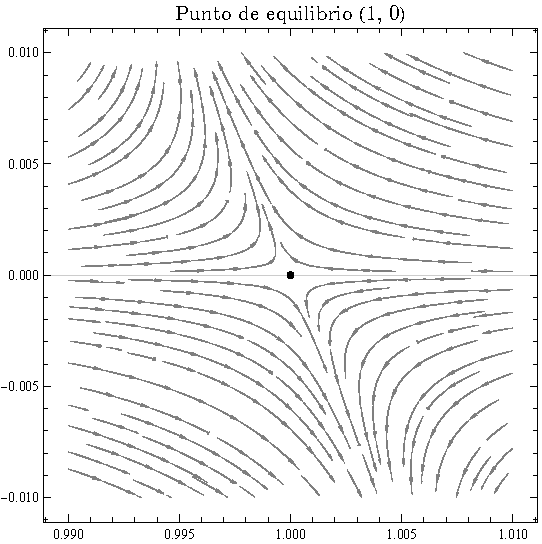
\includegraphics[width=.5\textwidth]{img/puntoDeEquilibrio(1,0).pdf}
	\caption{Punto de equilibrio $(1, 0)$ para valores paramétricos aleatorios.}
	\label{fig: eq(1,0)Modelo2}
\end{figure}

\subsection{Estabilidad del punto de equilibrio $(0,0)$}
Al evaluar el origen en la matriz \eqref{eq:jacobianaModelo2} obtenemos
\begin{equation*}
	Df(0,0) =
	\begin{bmatrix}
		0 & 0 \\
		0 & 0
	\end{bmatrix}.
	\label{eq:jacobianaModelo2En(0,0)}
\end{equation*}
En particular, para este punto crítico al obtener la matriz nula, deducimos que $(0,0)$ es un punto no hiperbólico y degenerado, por lo que no es posible determinar la estabilidad de este punto por medio de la linealización ni el teorema de la variedad central, por ello, para analizar el comportamiento de este punto de equilibrio se recurrirá a desingularizarlo a través del método de blowing-up polar. \\

\noindent Para ello, escribamos el sistema \eqref{eq: modelo2} en coordenadas polares. Sustituyendo $u = r \cos\theta$ y $v = r \sin\theta$, obtenemos que $r^{2}=u^{2}+v^{2} \;\text{ y }\; \theta = \arctg\left(\dfrac{v}{u}\right)$ con $u\neq0$. Derivando con respecto al tiempo $\tau$: $$\dot{r}=\cos\theta\dot{u} + \sin\theta\dot{v} \;\text{ y }\; \dot{\theta}=\dfrac{\dot{v}\cos\theta-\dot{u}\sin\theta}{r}.$$ Reemplazando $\dot{u}$ y $\dot{v}$ obtenemos el sistema:
\begin{equation*}
	\begin{cases}
		\dot{r} &= r^{2} g_1(r, \theta), \\
		\dot{\theta} &= r g_2(r, \theta),
	\end{cases}
\end{equation*}
donde
\begin{equation*}
	\begin{aligned}
		g_1(r, \theta) &= -Qr^{2}\cos^{4}\theta\sin\theta- r^{3}\cos^{6}\theta+ r^{2}\cos^{5}\theta \\ &-A^{2}r\cos^{4}\theta+ A^{2}\cos^{3}\theta + Br^{2}\cos^{3}\theta\sin^{2}\theta \\ &-Br^{2}\cos^{2}\theta\sin^{3}\theta+ A^{2}B\cos\theta\sin^{2}\theta- A^{2}B\sin^{3}\theta,
		\\
		g_2(r, \theta) &= Br^{2}\cos^{4}\theta\sin\theta- Br^{2}\cos^{3}\theta\sin^{2}\theta+ A^{2}B\cos^{2}\theta\sin\theta \\ &-A^{2}B\cos\theta\sin^{2}\theta+ Qr^{2}\cos^{3}\theta\sin^{2}\theta + r^{3}\cos^{5}\theta\sin\theta \\ &-r^{2}\cos^{4}\theta\sin\theta+ A^{2}r\cos^{3}\theta\sin\theta- A^{2}\cos^{2}\theta\sin\theta,
	\end{aligned}
\end{equation*}
es decir, obtuvimos el campo vectorial $$\tilde{Y_{\eta}}(r,\theta) = r^{2}g_1(r,\theta) \partial_r + rg_2(r,\theta) \partial_\theta.$$ Dividiendo por $r$ obtenemos un nuevo campo $$\bar{Y_{\eta}}(r,\theta) = rg_1(r,\theta) \partial_r + g_2(r,\theta) \partial_\theta,$$ el cual, en $\{r=0\}$ es cualitativamente equivalente a una vecindad del origen del campo vectorial $Y_{\eta}$ dado por el sistema \eqref{eq: modelo2}, es decir, basta analizar el retrato fase del campo vectorial:
\begin{equation*}
	\begin{aligned}
		\bar{Y_{\eta}}(0,\theta) = g_2(0, \theta) &= A^{2}B\cos^{2}\theta\sin\theta - A^{2}B\cos\theta\sin^{2}\theta- A^{2}\cos^{2}\theta\sin\theta \\
		&= A^{2}\cos\theta\sin\theta (B\cos\theta-B\sin\theta-\cos\theta),
	\end{aligned}
\end{equation*}
para determinar el comportamiento del sistema \eqref{eq: modelo2} en una vecindad del origen. \\

\noindent Hallemos los puntos críticos de $\bar{Y_{\eta}}(0,\theta)$ ubicados en el primer cuadrante. Igualando el campo vectorial $\bar{Y_{\eta}}(0,\theta)$ a cero, debe ocurrir al menos que $\cos\theta$, $\sin\theta$ o $B\cos\theta-B\sin\theta-\cos\theta$ se anule. Esto ocurre para los valores $\theta_1 = 0, \; \theta_2 = \dfrac{\pi}{2}$ y los que cumplan la igualdad $$\dfrac{B-1}{B}\cos\theta=\sin\theta,$$ es decir, $\theta_3 = \arctg\left( \dfrac{B-1}{B} \right)$; aquí, notemos que el escenario de relevancia es para el caso $B>1$, pues para $B=1$ estaríamos hablando de $\theta_3 = \theta_1 = 0$ y para $B<1$, $\theta_3$ no estaría en el primer cuadrante. \\

\noindent La matriz jacobiana del campo $\bar{Y}_{\eta}(0,\theta)$ esta dada por
\begin{equation*}
	D\bar{Y_{\eta}}(0,\theta) =
	\begin{bmatrix}
		b_{11}(\theta)  & 0\\
		A^{2}\cos^{3}\theta\sin\theta & b_{22}(\theta)
	\end{bmatrix},
	\label{eq:jacobianaModelo2Polar}
\end{equation*}
con
\begin{equation*}
	\begin{aligned}
		b_{11}(\theta) &= A^{2}\cos^{3}\theta + A^{2}B[\cos\theta\sin^{2}\theta - \sin^{3}\theta], \\
		b_{22}(\theta) &= A^{2}B[\sin^{3}\theta + \cos^{3}\theta - 2\sin^{2}\theta\cos\theta - 2\sin\theta\cos^{2}\theta] \\
		&+ A^{2}[2\cos\theta\sin^{2}\theta - \cos^{3}\theta].
	\end{aligned}
\end{equation*}

\subsubsection*{Estabilidad en $(0, \theta_1)$ con $\theta_1=0$}
En el punto crítico $(0,\theta_1)$, obtenemos la matriz:
\begin{equation*}
	D\bar{Y_{\eta}}(0,\theta_1) =
	\begin{bmatrix}
		A^{2}  & 0 \\
		0 & A^{2}(B-1)
	\end{bmatrix},
	\label{eq:jacobianaModelo2PolarEn(0,0)}
\end{equation*}
con valores propios $\lambda_r = A^{2}>0, \; \lambda_\theta = A^{2}(B-1),$ radial y tangencial, respectivamente. Por lo tanto, $(0, \theta_1)$ es un punto silla de $\bar{Y_{\eta}}(0,\theta)$ si \linebreak $B<1$, es una fuente si $B>1$ y un punto crítico no hiperbólico si $B=1$. Aquí observamos qué la estabilidad de este punto de equilibrio depende del parámetro $B$, la cual influirá en la estructura cualitativa del campo $\bar{Y_{\eta}}(r,\theta)$ y por ende en la del sistema \eqref{eq: modelo2}. \\ % Así, obtenemos que hay un cambio cualitativo en el valor de bifurcación $B=1$, posteriormente se analizará que tipo de bifurcación se presenta en este modelo.

\noindent Ahora, debido a que en el caso $B=1$ el punto $(0,\theta_1)$ es un punto no hiperbólico, no es posible aplicar el teorema de Harmant-Grobman para determinar su estabilidad y por ello recurriremos al teorema de la variedad central (TVC). \\

\noindent Recordemos que el TVC nos garantiza la existencia de una curva invariante $r = h(\theta)$ que define la variedad central en una vecindad del origen, cuyo flujo esta determinado por la ecuación diferencial $\dot{\theta} = g_2(h(\theta), \theta)$. En nuestro caso, al estar determinando la estabilidad de los puntos críticos en el circulo ${r = 0}$, esto conlleva a la omisión de tener que especificar como esta definida la curva invariante $h(\theta)$. Por ende, para precisar la estabilidad del origen para el caso $B = 1$, solo basta determinar el flujo de la ecuación diferencial
\begin{equation}
	\dot{\theta} = g_2(0, \theta) = - A^2 \sin ^2 \theta \cos \theta;
	\label{eq:flujotheta0}
\end{equation}
para ello, hallemos los primeros términos de la expansión en serie de Taylor de $ - A^2 \sin ^2 \theta \cos \theta$ alrededor de $\theta = 0$. Como
$$
	\sin \theta = \theta - \dfrac{\theta^3}{3!} + \mathcal{O}(\theta^ 5), \quad
	\sin^2 \theta = \theta^2 + \mathcal{O}(\theta^ 4) \quad \text{y} \quad
	\cos \theta = 1 - \dfrac{\theta^2}{2!} + \mathcal{O}(\theta^ 4),
$$
%
%\begin{equation*}
%	\begin{aligned}
%		\sin \theta &= \theta - \dfrac{\theta^3}{3!} + \mathcal{O}(\theta^ 5) \\
%		\sin^2 \theta &= \theta^2 + \mathcal{O}(\theta^ 4) \\
%		\cos \theta &= 1 - \dfrac{\theta^2}{2!} + \mathcal{O}(\theta^ 4)
%	\end{aligned}
%\end{equation*}
entonces, de \eqref{eq:flujotheta0} tenemos 
\begin{equation*}
	\dot{\theta} = - A^2 \sin ^2 \theta \cos \theta = -A^2 \theta^2 + \mathcal{O}(\theta^ 4).
\end{equation*}
Así, como el orden del primer termino de la expansión es par, se concluye que $(0, \theta_1)$ para el caso $B=1$ es un punto silla-nodo de $\bar{Y_{\eta}}(0,\theta)$ \cite{perko2001}[p.~157].

\subsubsection*{Estabilidad en $(0, \theta_2)$ con $\theta_2=\pi/2$}

Tenemos que:
\begin{equation*}
	D\bar{Y_{\eta}}(0,\theta_2) =
	\begin{bmatrix}
			-A^{2}B  & 0 \\
			0 & A^{2}B
		\end{bmatrix},
	\label{eq:jacobianaModelo2PolarEn(0,pi2)}
\end{equation*}
con valores propios $\lambda_r = -A^{2}B<0$ y $\lambda_\theta = A^{2}B>0$. Por lo tanto, $\left(0,\theta_2\right)$ es un punto silla de $\bar{Y_{\eta}}(0,\theta)$.

\subsubsection*{Estabilidad en $(0, \theta_3)$ con $\theta_3=\arctg\left((B-1)/B\right)$}

Denotando $k = \dfrac{B-1}{B}$, donde $B>1$, y tomando en cuenta las identidades
\begin{equation*}
	\begin{aligned}
		\sin(\theta_3) &= \dfrac{k}{\sqrt{1+k^{2}}}, \\
		\cos(\theta_3) &= \dfrac{1}{\sqrt{1+k^{2}}},
	\end{aligned}
\end{equation*}
llegamos a que
\begin{equation*}
	D\bar{Y_{\eta}}(0,\theta_3) = \dfrac{A^{2}}{(1+k^{2})^{3/2}}
	\begin{bmatrix}
		b_{11}(\theta_3) & 0 \\
		\dfrac{k}{(1+k^{2})^{1/2}} & b_{22}(\theta_3)
	\end{bmatrix},
\end{equation*}
donde
\begin{equation*}
	\begin{aligned}
		b_{11}(\theta_3) &= 1 + Bk^{2}(1-k), \\
		b_{22}(\theta_3) &= B(k^{3}-2k+1) -2k^{2}(B-1) - 1,
	\end{aligned}
\end{equation*}
reemplazando $k = \dfrac{B-1}{B}$, obtenemos que:
\begin{equation*}
	\begin{aligned}
		b_{11}(\theta_3) &= 1 + B\dfrac{(B-1)^{2}}{B^{2}}\left(1-\dfrac{B-1}{B}\right) \\ 
		&=\dfrac{2B^{2}-2B+1}{B^{2}}, \\
		b_{22}(\theta_3) &= B\left(\dfrac{(B-1)^{3}}{B^{3}}-2\dfrac{B-1}{B}+1\right) -2\dfrac{(B-1)^{2}}{B^{2}}(B-1) - 1 \\ 
		&= -\dfrac{(B-1)(2B^{2}-2B+1)}{B}, \\
		1+k^{2} &= \dfrac{2B^{2}-2B+1}{B^{2}}.
	\end{aligned}
\end{equation*}
Así,
\begin{equation}
	D\bar{Y_{\eta}}\left(0,\theta_3\right) =
	\begin{bmatrix}
		\dfrac{A^2 B}{(2B^{2}-2B+1)^{1/2}} & 0 \\
		\dfrac{A^2 B^4 (B-1)}{(2B^{2}-2B+1)^{2}} & -\dfrac{A^2 B^2 (B-1)}{(2B^{2}-2B+1)^{1/2}}
	\end{bmatrix}.
	\label{eq:jacobianaModelo2PolarEn(0,b)}
\end{equation}
Con valores propios $$\lambda_r = \dfrac{A^2 B}{(2B^{2}-2B+1)^{1/2}}>0 \quad \text{y} \quad \lambda_\theta = -\dfrac{A^2 B^2 (B-1)}{(2B^{2}-2B+1)^{1/2}}<0.$$ Por lo tanto, $(0,\theta_3)$ es un punto silla de $\bar{Y_{\eta}}(0,\theta)$. \\

Luego de hallar la estabilidad de cada punto crítico de $\bar{Y_{\eta}}$, junto con sus respectivos valores propios radiales y tangenciales, podemos determinar como se comporta cualitativamente el origen del campo $Y_{\eta}$ en una cierta vecindad. Este comportamiento se puede evidenciar en la figura \ref{fig: BlowUp Modelo 2}, en donde, para el caso $B\leq1$ vemos que el primer cuadrante consta de un único sector hiperbólico, y para $B>1$ de uno parabólico y uno hiperbólico. Recordemos que la finalidad de la técnica del blow-up es determinar el comportamiento del origen en $Y_{\eta}$, en sí, este proceso nos permite determinar que trayectorias entran o salen del origen, y son determinadas por la pendiente $\tan \theta^*$, donde $\theta^*$ es un punto crítico de $\bar{Y_{\eta}}$. Por ende, en el primer cuadrante de $Y_{\eta}$ hay tres de estas trayectorias: $v=0$ que corresponde a la orbita con pendiente $\tan\theta_1=0$, $u=0$ que corresponde a la orbita con pendiente $\tan\theta_2= \infty$ y la orbita determinada por la pendiente $\tan\theta_3=\dfrac{B-1}{B}$, la cual solo se da para el caso $B>1$, y además define una curva separatriz puesto que divide el retrato de fase en dos sectores con comportamientos cualitativos distintos (parabólico e hiperbólico).

\begin{figure}[H]
	\centering
	\begin{subfigure}{0.305\textwidth}
		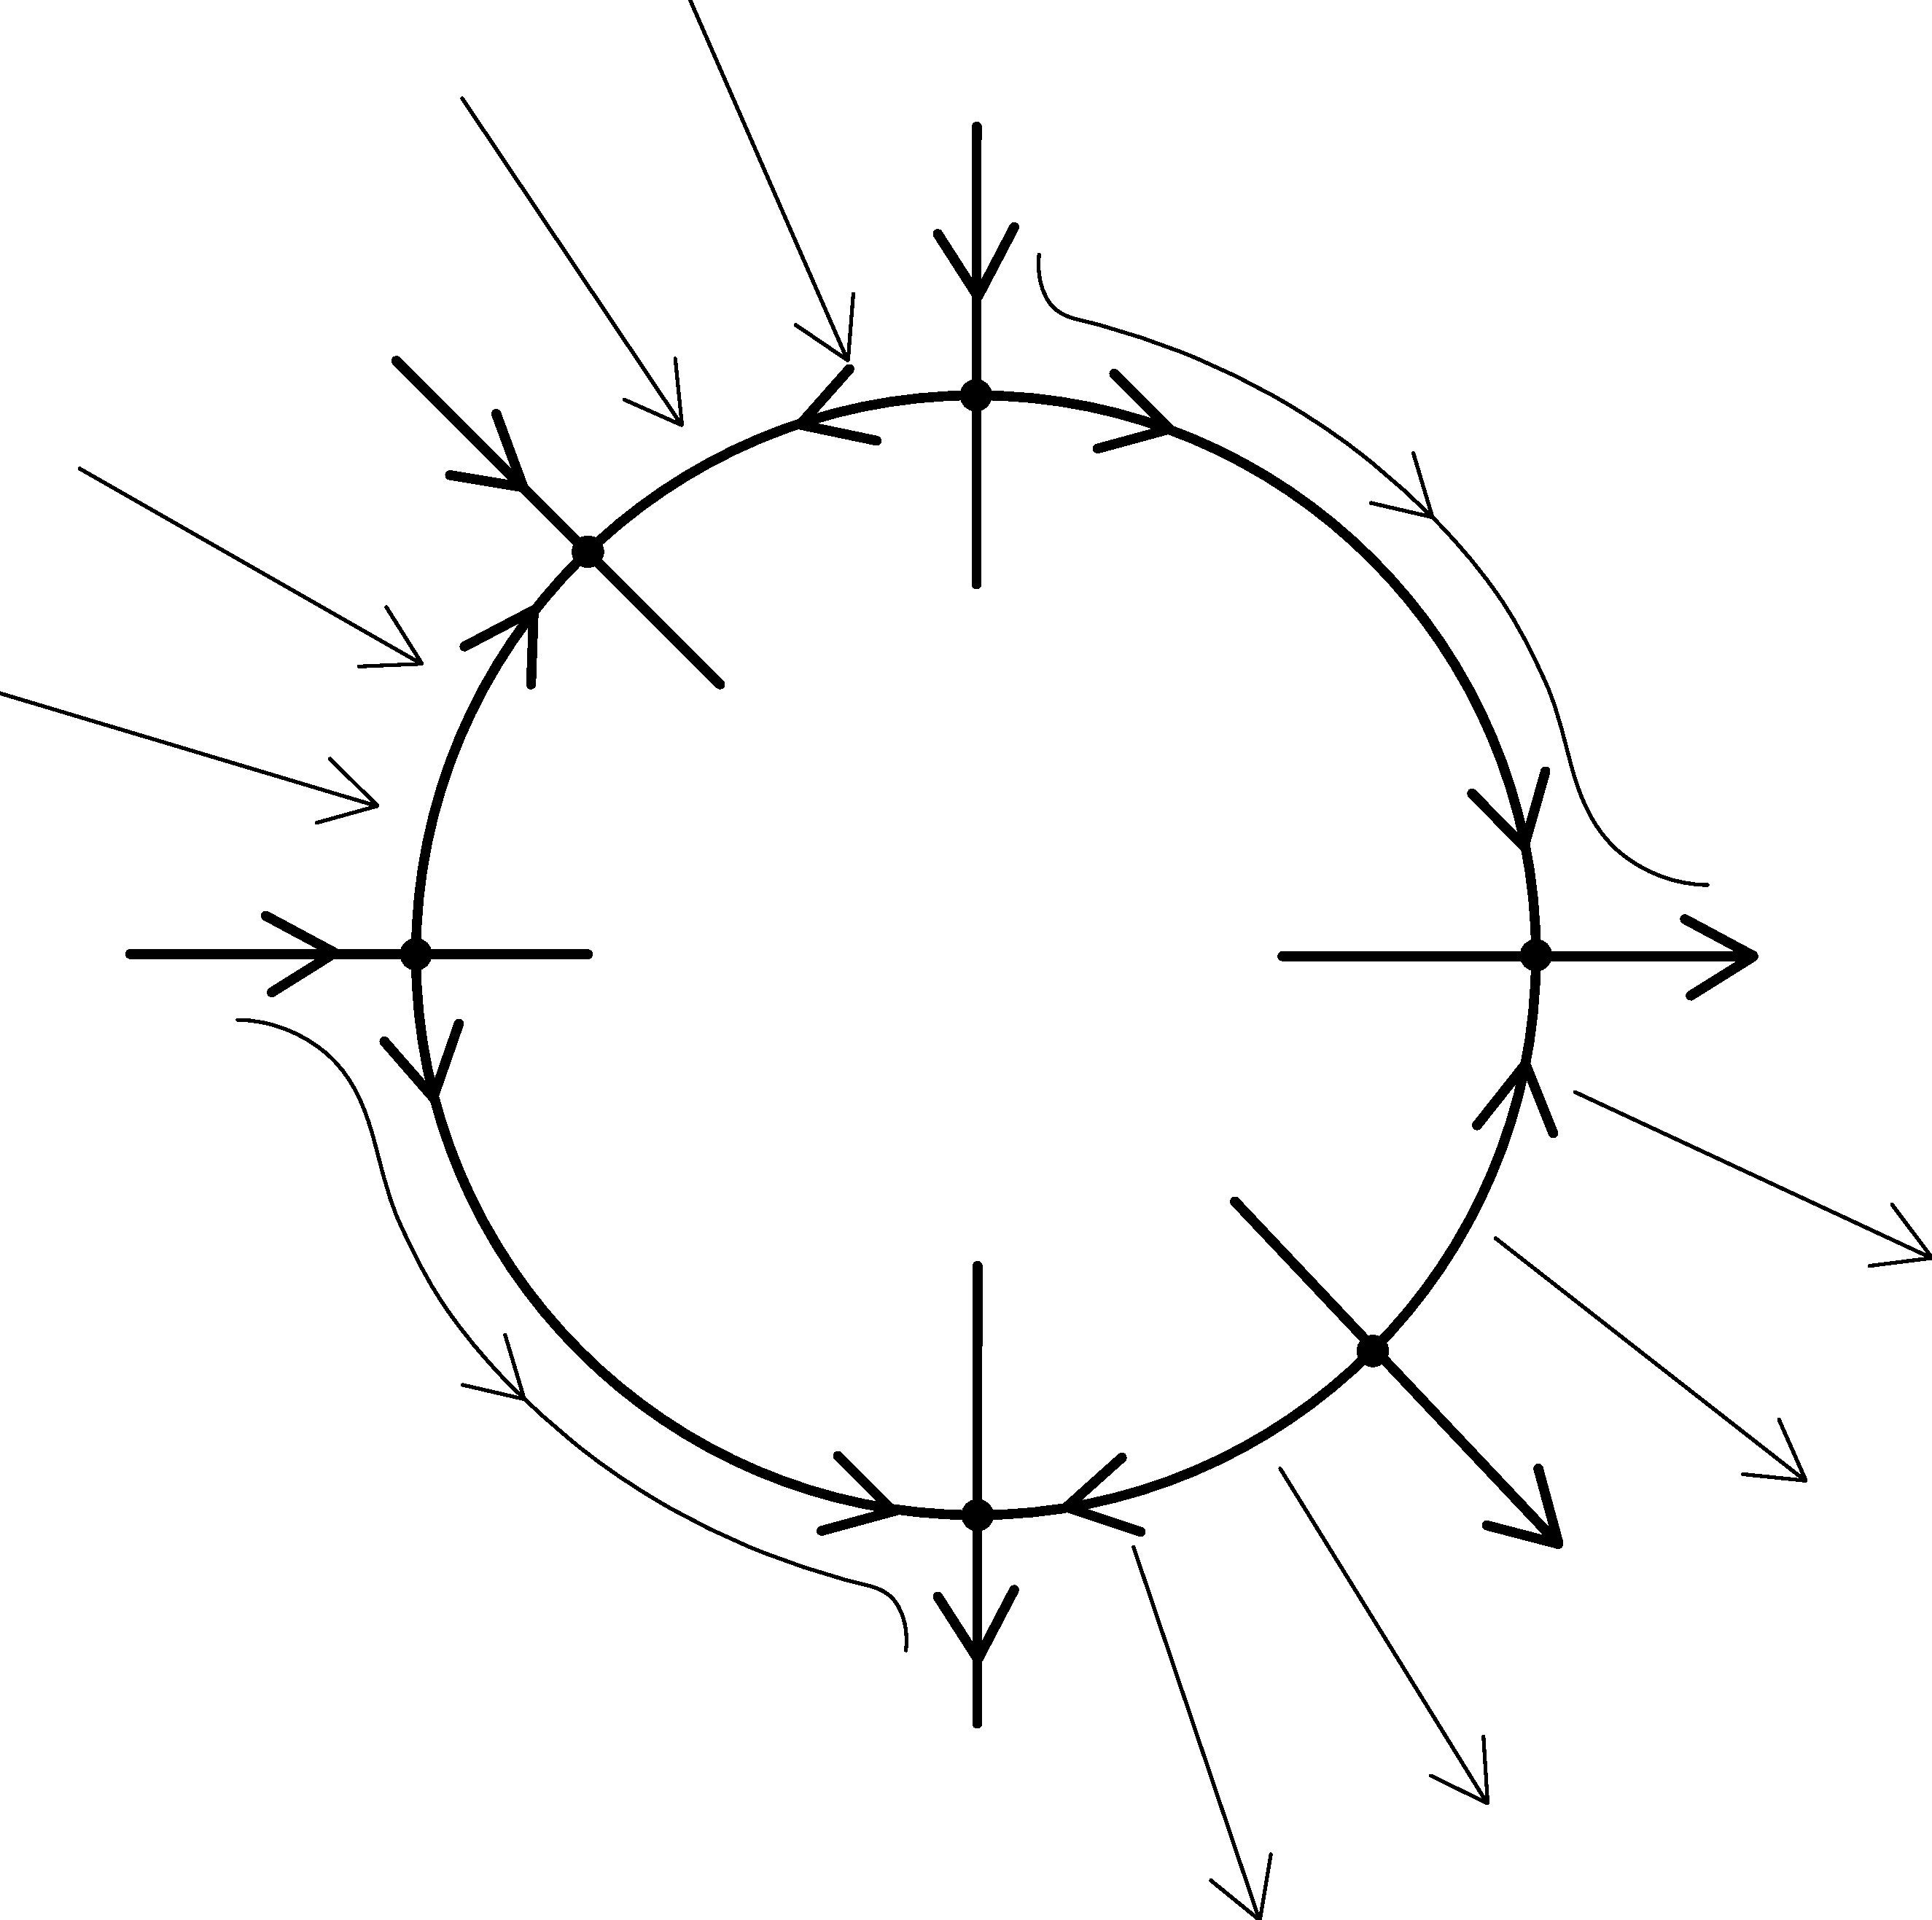
\includegraphics[width=\textwidth]{img/blowingUpPolar(Bmen1).pdf}
		\caption{$B < 1$.}
		\label{fig: BlowUp Modelo 2 B<1}
	\end{subfigure}
	\hfill
	\begin{subfigure}{0.305\textwidth}
		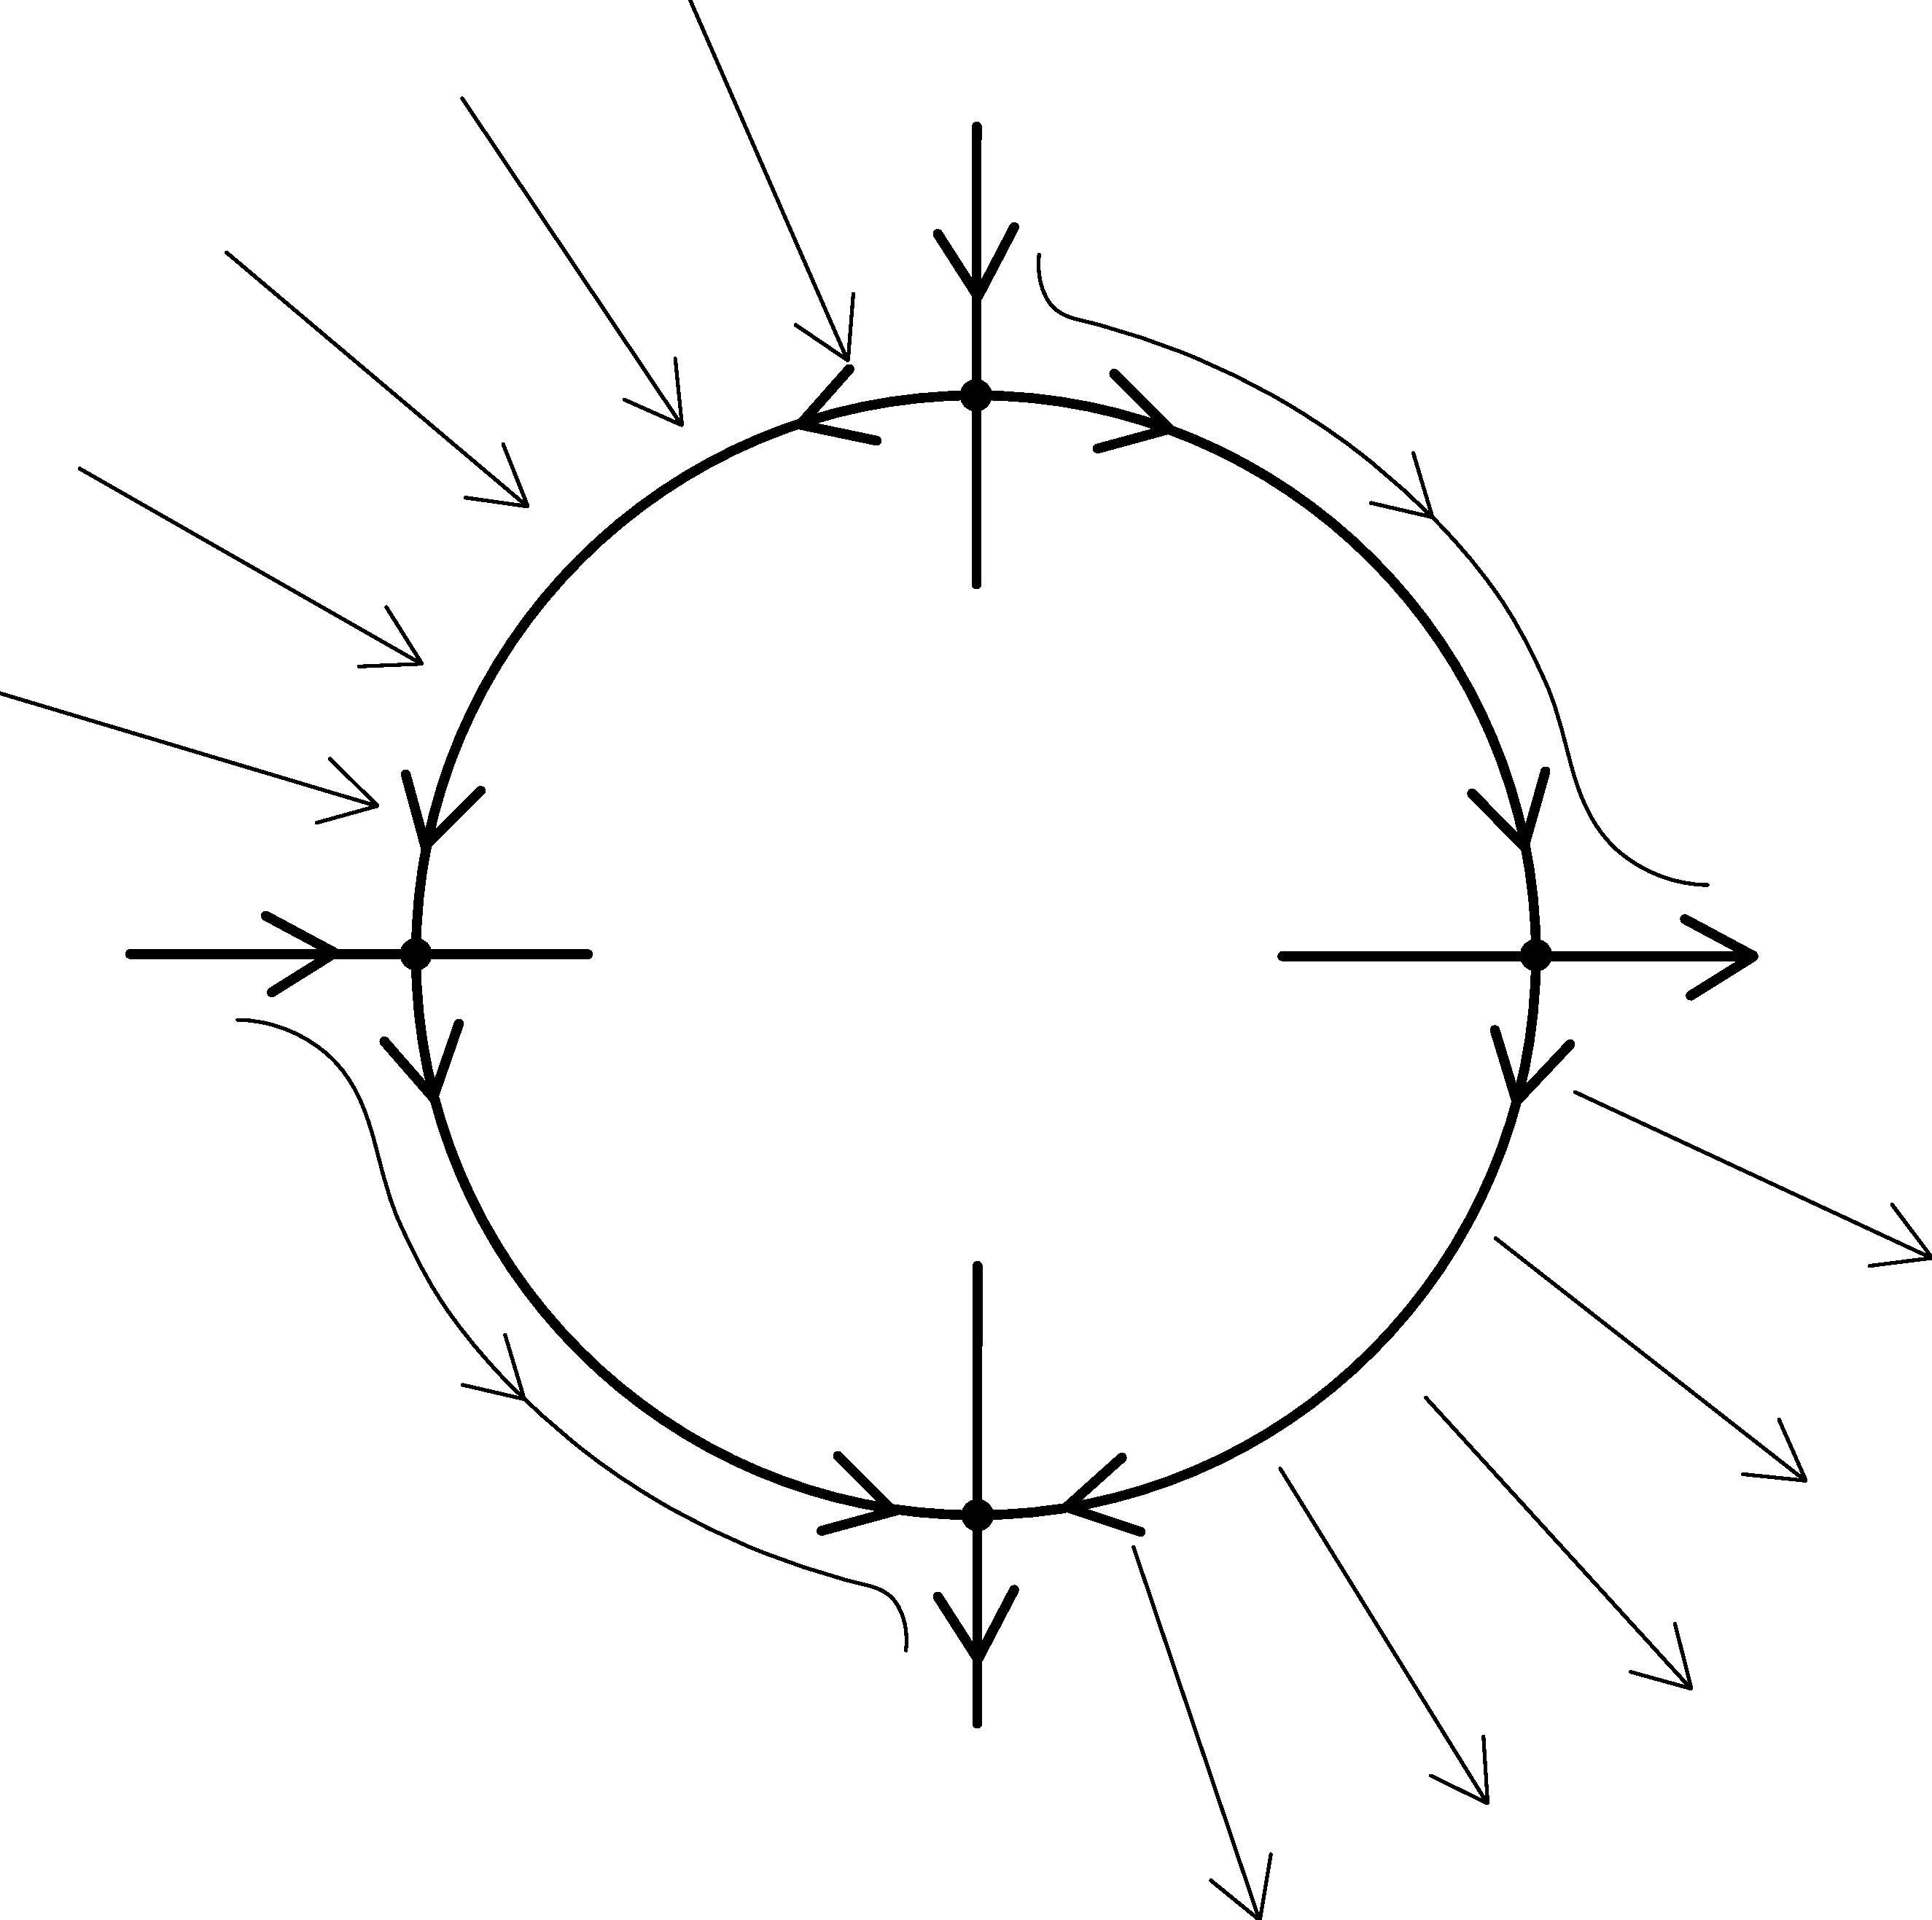
\includegraphics[width=\textwidth]{img/blowingUpPolar(Bigu1).pdf}
		\caption{$B = 1$.}
		\label{fig: BlowUp Modelo 2 B=1}
	\end{subfigure}
	\hfill
	\begin{subfigure}{0.35\textwidth}
		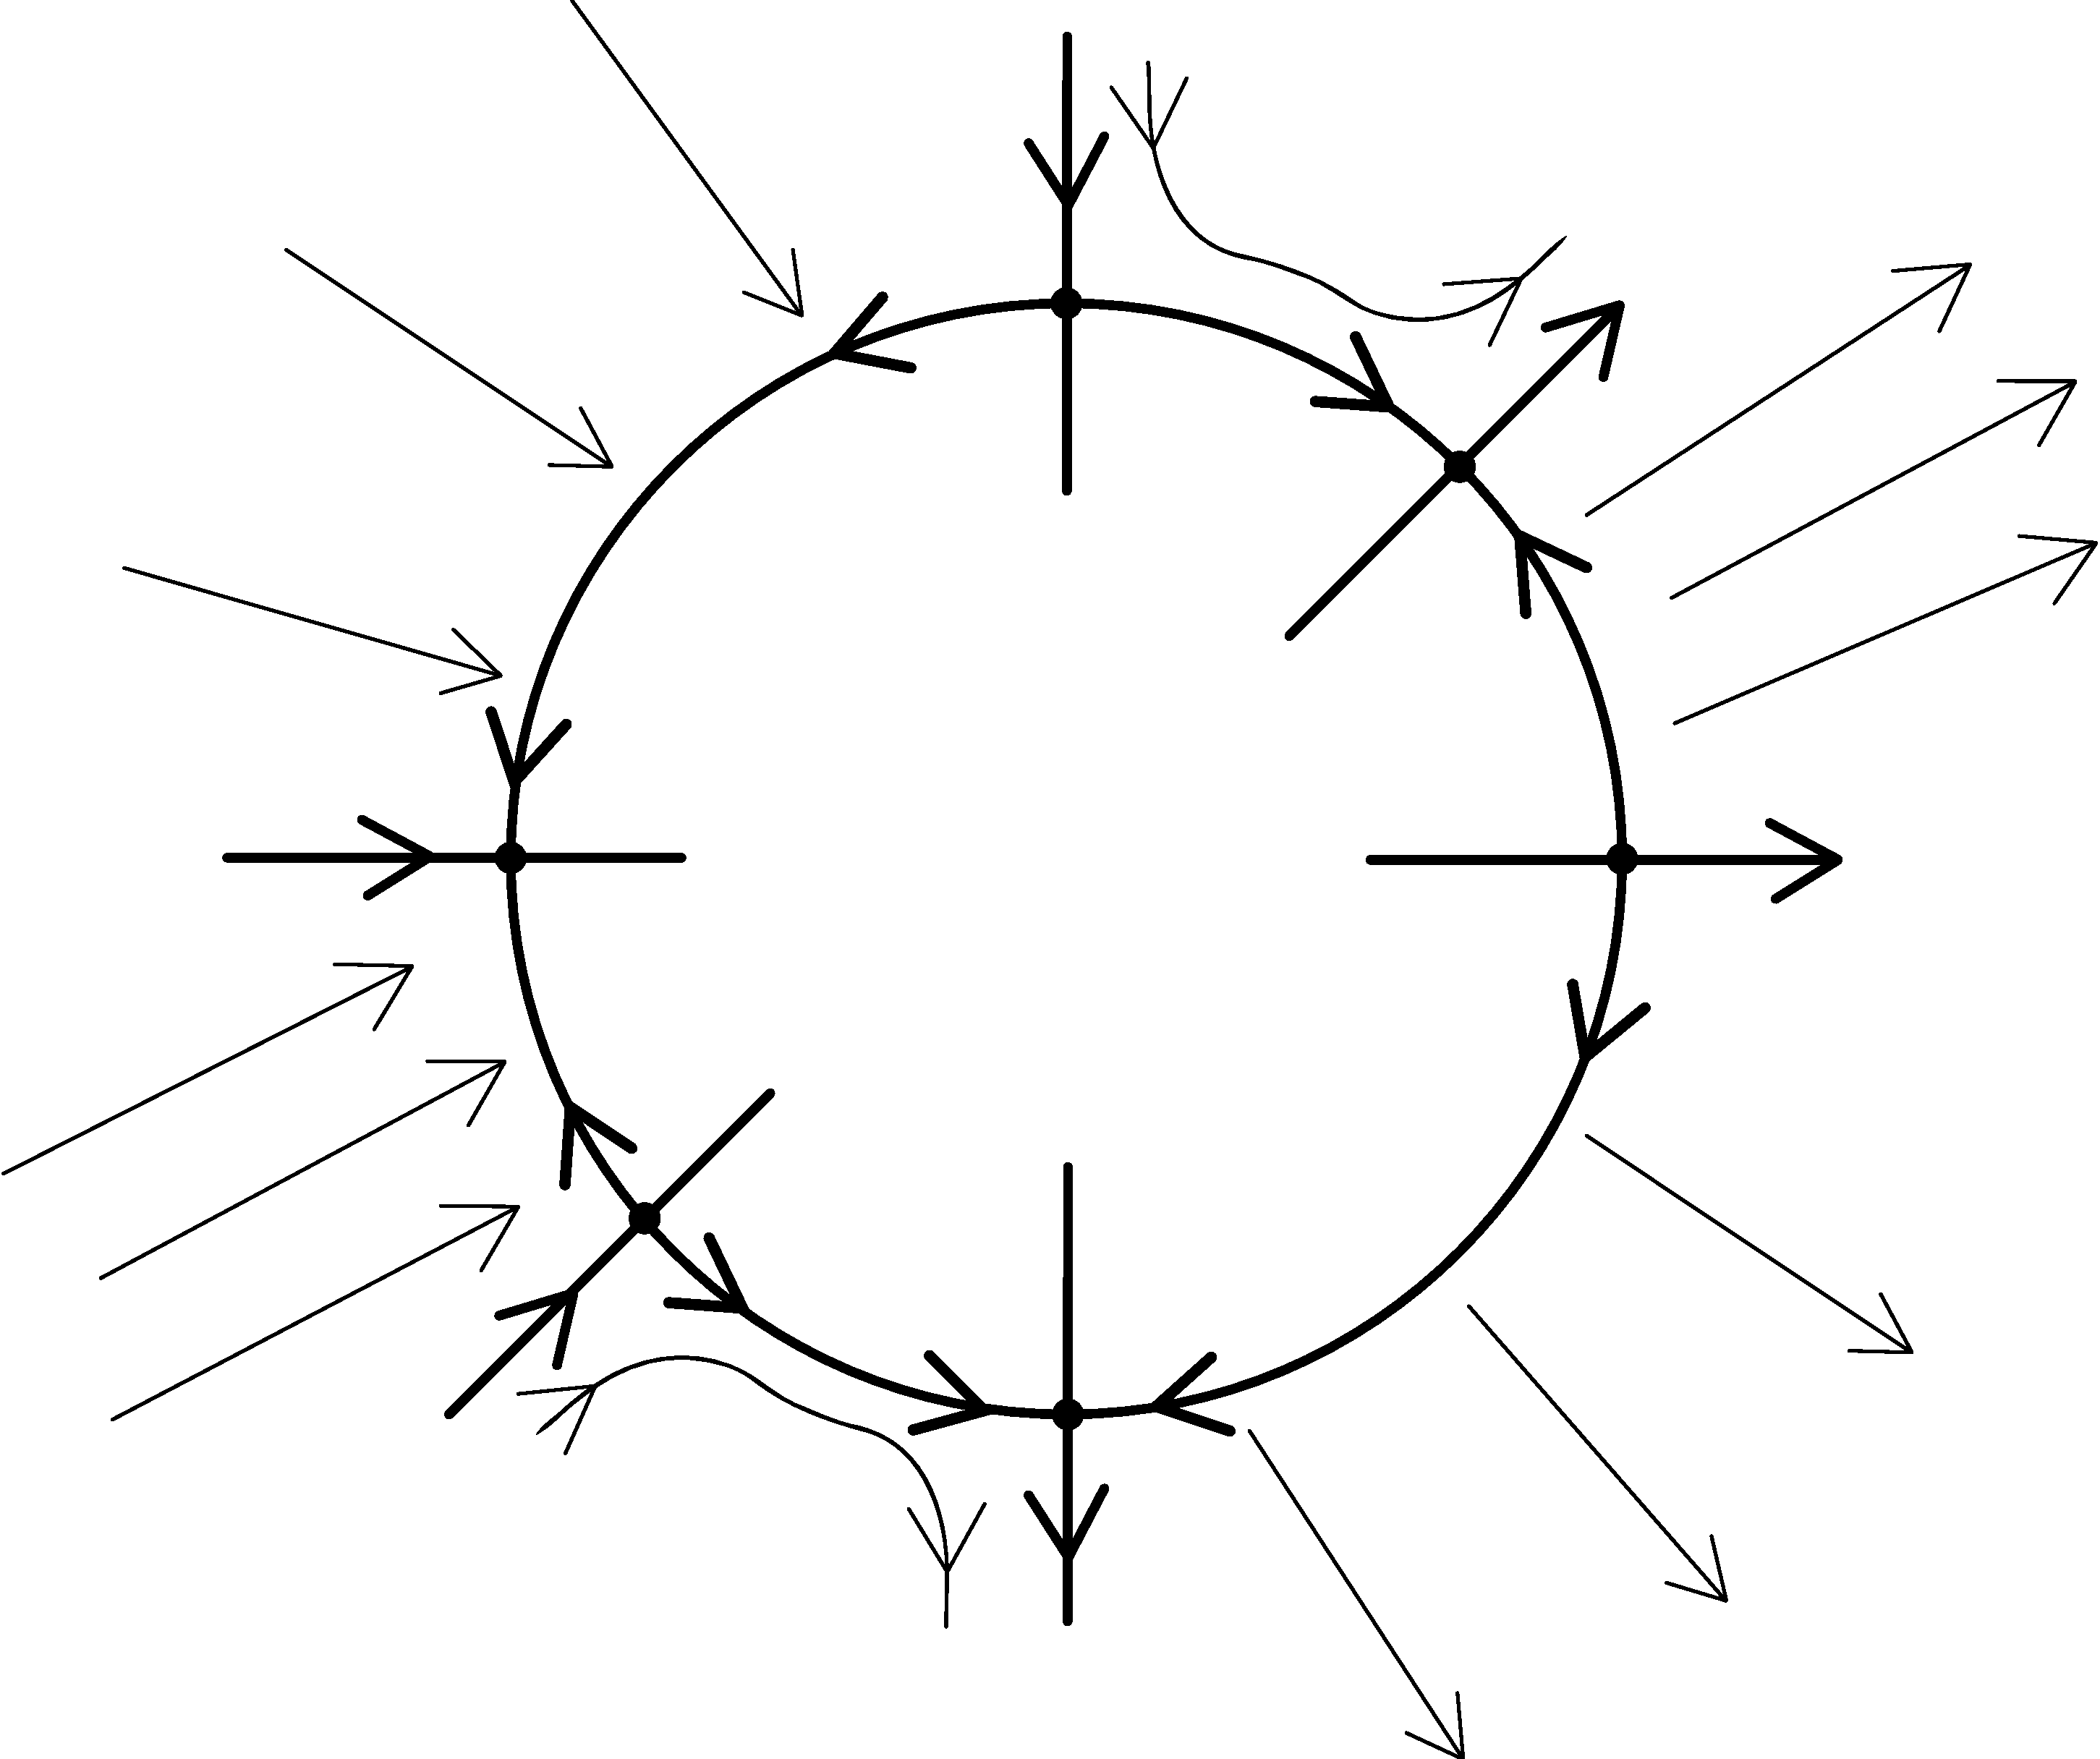
\includegraphics[width=\textwidth]{img/blowingUpPolar(Bmay1).pdf}
		\caption{$B > 1$.}
		\label{fig: BlowUp Modelo 2 B>1}
	\end{subfigure}
	\caption{Blow-up en el origen del sistema \eqref{eq: modelo2} para diferentes valores de $B$.}
	\label{fig: BlowUp Modelo 2}
\end{figure}

\begin{remark}
	De \eqref{eq:jacobianaModelo2PolarEn(0,b)} deducimos que para el caso $B<1$, $\theta_3$ está ubicado en el cuarto cuadrante y es un punto repulsor o fuente del campo $\bar{Y_{\eta}}(0,\theta)$, la estabilidad de los puntos antipodales ($\theta + \pi$) que son mostrados en la \autoref{fig: BlowUp Modelo 2}, pueden ser determinados a partir de la matriz jacobiana $D\bar{Y_{\eta}}(0,\theta + \pi)$ cuyos valores propios solo difieren del signo de los autovalores de $D\bar{Y_{\eta}}(0,\theta)$. La formula del índice de Poincaré $$i=\frac{e-h}{2}+1=0,$$ donde $e$ denota la cantidad de sectores elípticos y $h$ la de sectores hiperbólicos del origen \cite[p.~179]{Dumortier2006}, nos indica que este punto en el sistema \eqref{eq: modelo2} tiene un comportamiento local tipo silla-nodo.
\end{remark}

\begin{figure}[H]
	\centering
	\begin{subfigure}{0.49\textwidth}
		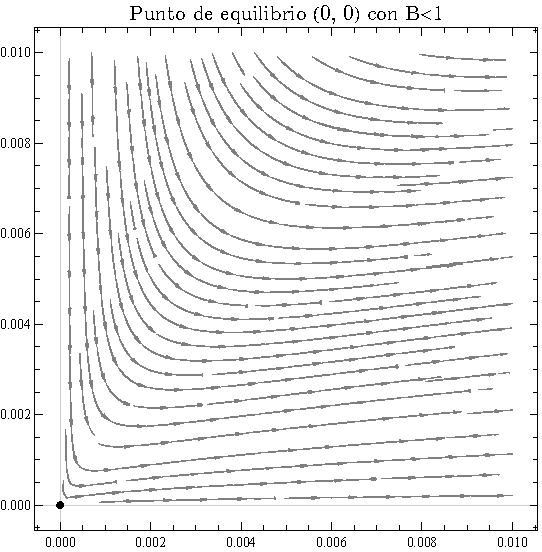
\includegraphics[width=\textwidth]{img/puntoDeEquilibrio(0,0)conBmenor1.pdf}
		\caption{Retrato fase del sistema \eqref{eq: modelo2} cerca al origen para valores paramétricos aleatorios con $B < 1$.}
		\label{fig: eq(0,0)Modelo2Bmenor1}
	\end{subfigure}
	\hfill
	\begin{subfigure}{0.49\textwidth}
		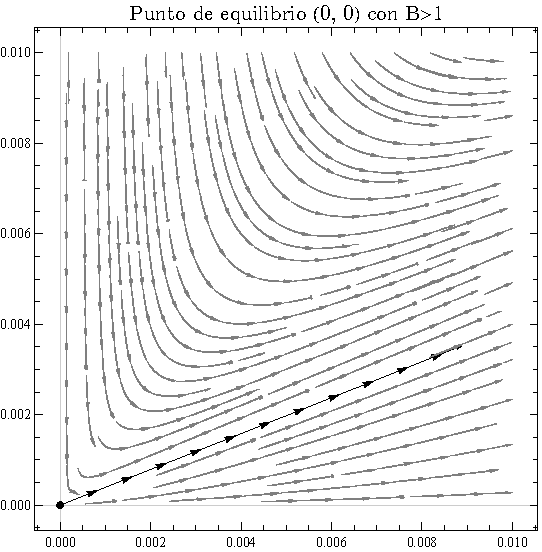
\includegraphics[width=\textwidth]{img/puntoDeEquilibrio(0,0)conBmayor1.pdf}
		\caption{Retrato fase del sistema \eqref{eq: modelo2} cerca al origen para valores paramétricos aleatorios con $B > 1$.}
		\label{fig: eq(0,0)Modelo2Bmayor1}
	\end{subfigure}
	\caption{Retrato fase del sistema \eqref{eq: modelo2} cerca al origen.}
	\label{fig: eq(0,0)Modelo2}
\end{figure}

\subsection{Estabilidad del punto de equilibrio $(H,H)$}
\label{sec: HH}
Con el fin de reducir los posibles casos que se pueden dar en los valores propios, reduciremos la cantidad de parámetros realizando la sustitución
\begin{equation}
	Q=\dfrac{(1-H)(A^2+H^{2})}{H^{2}},
	\label{eq: Q}
\end{equation}
anteriormente discutida en la \Cref{pro:exitenciaH}. Así, tendríamos que la matriz jacobiana del sistema \eqref{eq: modelo2} en $(H,H)$ es:
\begin{equation}
	Df(H,H) =
	\begin{bmatrix}
		-H(H^{2}(2H-1)+A^2) & -H(1-H)(A^2+H^2) \\
		BH(A^{2}+H^{2}) & -BH(A^{2}+H^{2})
	\end{bmatrix}.
	\label{eq:jacobianaModelo2En(H,H)}
\end{equation}
Los valores propios se hallan del polinomio característico $$\lambda^2 - \operatorname{tr}(M) \lambda + \det(M) = 0,$$ con $M = Df(H,H)$, estos es:
\begin{equation*}
	\lambda(\mu) = \dfrac{\operatorname{tr}(M) \pm \sqrt{\Delta}}{2},
\end{equation*}
donde $\mu = (A, \; B)$, $\Delta = (\operatorname{tr}(M))^2 - 4\det(M)$ y
\begin{equation*}
	\begin{aligned}
		\operatorname{tr}(M) &= -H(B(A^{2}+H^{2})+H^{2}(2H-1)+A^2), \\
		\det(M) &= BH^2(A^2+H^2)(H^3+A^2(2-H)).
	\end{aligned}
\end{equation*}
Como $H \in (0, 1)$, $\det(M)>0$ por lo que $(H,H)$ es un punto no degenerado e hiperbólico o un centro lineal; además, no puede ser un punto silla. Así la estabilidad estaría determinada por el signo de la traza y del discriminante $\Delta$, para ello notemos que $\operatorname{tr}(M)=0$ si
\begin{equation}
	B = \dfrac{H^2(1-2H) - A^2}{A^2 + H^2} := B_c,
	\label{eq: Bcritico}
\end{equation}
y puesto que $B>0$, esto se da bajo las restricciones: $$H<1/2 \; \text{ y } \; A^2 < H^2(1-2H).$$ Este hecho da paso a los siguientes casos:
\begin{itemize}
	\item Si $B<B_c$ y
	\subitem $\Delta < 0$, $(H,H)$ es un foco inestable.
	\subitem $\Delta = 0$, $(H,H)$ es un nodo degenerado inestable.
	\subitem $\Delta > 0$, $(H,H)$ es un nodo inestable.
	\item Si $B=B_c$, $(H,H)$ es un centro lineal.
	\item Si $B>B_c$ y
	\subitem $\Delta < 0$, $(H,H)$ es un foco estable.
	\subitem $\Delta = 0$, $(H,H)$ es un nodo degenerado estable.
	\subitem $\Delta > 0$, $(H,H)$ es un nodo estable.
\end{itemize}				

Dado que la linealización no garantiza que $(H, H)$ sea un punto centro para el caso $B=B_c$, ya que en este caso el punto de equilibrio es no hiperbólico, se es de importancia verificar si $(H, H)$ es un punto centro o un foco débil en el sistema no linealizado. Con el propósito de validar la estructura cualitativa en este caso, calcularemos el primer número de Lyapunov.
%; esto no es sólo con este fin, sino con el de validar que tipo de bifurcación de Hopf se nos presenta, puesto que dicha característica esta garantizada debido al siguiente teorema.

\begin{figure}[H]
	\centering
	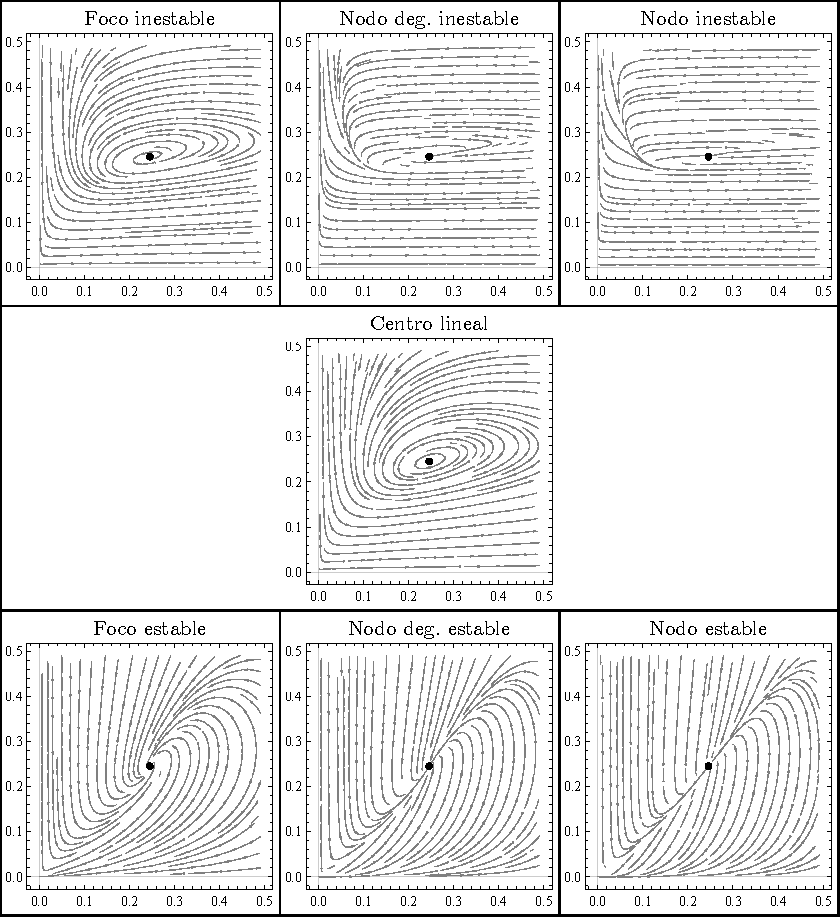
\includegraphics[width=.85\textwidth]{img/puntoDeEquilibrio(H,H).pdf}
	\caption{Punto de equilibrio $(H, H)$ para diferentes valores paramétricos.}
	\label{fig: eq(H,H)Modelo2}
\end{figure}

\subsubsection{Calculo del primer coeficiente de Lyapunov}
Para proceder con el calculo del primer coeficiente de Lyapunov, debemos trasladar el punto de equilibrio $(H, H)$ al origen. Para ello, realicemos las sustituciones $u = \bar{u} + H$ y $v = \bar{v} + H$ en el sistema \eqref{eq: modelo2} y reemplazamos el valor crítico $B_c$ con el fin de obtener $(H,H)$ como un centro lineal (Valores propios complejos puros en la matriz jacobiana del sistema evaluada en el punto crítico). Estos cambios se ven reflejados de la siguiente manera:
\begin{equation}
	W_{\eta}:
	\begin{cases}
		\dfrac{d\bar{u}}{d \tau} = h_1(\bar{u}, \bar{v}), \\ \\
		\dfrac{d\bar{v}}{d \tau} = h_2(\bar{u}, \bar{v}),
	\end{cases}
	\label{eq: modelo2Hen0}
\end{equation}
donde
\begin{equation*}
	\begin{aligned}
		h_1(\bar{u}, \bar{v}) &= [(1 - \bar{u} - H)[(\bar{u} + H)^{2} + A^{2}] - Q (\bar{u} + H) (\bar{v} + H)](\bar{u} + H)^{2}, \\
		h_2(\bar{u}, \bar{v}) &= B_c(\bar{u} - \bar{v})[(\bar{u} + H)^{2} + A^{2}](\bar{v} + H).
	\end{aligned}
\end{equation*}
Por la igualdad \eqref{eq: Q}, la matriz jacobiana del sistema \eqref{eq: modelo2Hen0} en el origen estaría dada simplemente por la matriz \eqref{eq:jacobianaModelo2En(H,H)} sustituyendo $B=B_c$:
\begin{equation}
	Dh(0,0) =
	\begin{bmatrix}
	a & b \\
	a & - a
	\end{bmatrix},
	\label{eq:jacobianamodelo2Hen0}
\end{equation}
con
\begin{equation*}
	\begin{aligned}
		a &= H[H^{2}(1-2H)-A^2], \\
		b &= -H(1-H)(A^2+H^2).
	\end{aligned}
\end{equation*}
Como el origen es un punto crítico del sistema \eqref{eq: modelo2Hen0}, este puede expresarse como
\begin{equation}
	\left(\dfrac{d\bar{u}}{d \tau}, \dfrac{d\bar{v}}{d \tau}\right)^T=Dh(0,0)(\bar{v},\bar{v})^T+(F_1(\bar{v},\bar{v}), F_2(\bar{u},\bar{v}))^T,
	\label{eq: sistemal1}
\end{equation}
donde $(F_1, F_2)$ son las expansiones de Taylor en 0, de los terminos no lineales del sistema. El primer coeficiente de Lyapunov está dado por
\begin{equation}
	l_1 = \frac{1}{2 \omega^2}Re(i g_{20}g_{11} + \omega g_{21}),
	\label{eq: l1}
\end{equation}
donde las expresiones $ g_{20}, g_{11}$ y $g_{21}$ se determinan a partir del sistema \eqref{eq: sistemal1} transformado a la forma normal de Poincaré:
\begin{equation}
	\dot{z} = \omega i z + \sum_{2 \le k+l \le 3} \frac{1}{k!l!} g_{kl} z^k \bar{z}^l + O(|z|^4)
	\label{eq: normalForm}
\end{equation}
con $z=\langle p,(\bar{u},\bar{v}) \rangle$, donde $p=(p_1,p_2)$ es el autovector asociado al valor propio complejo puro $-\omega i$ de la matriz jacobiana $Dh(0,0)^T$, considerando el producto interno $\langle m,n \rangle = \bar{m}_1 n_1 + \bar{m}_2 n_2$. \\

Las expresiones necesarias para el cálculo del primer coeficiente de Lyapunov \eqref{eq: l1} también pueden determinarse a partir de las igualdades
\begin{equation}
	g_{20}=G_{zz}, \; g_{11}=G_{zw}, \; g_{21}=G_{zzw},
	\label{eq: derFunComplejaL1}
\end{equation}
con $G_{z z}, \;G_{z w}$ y $G_{z z w}$ dadas por las derivadas parciales evaluadas en \linebreak $z=w=0$ de la función de variable compleja
\begin{equation}
	G(z,w) = \bar{p_1}F_1(zq_1+w\bar{q_1}, zq_2+w\bar{q_2}) + \bar{p_2}F_2(zq_1+w\bar{q_1}, zq_2+w\bar{q_2}),
	\label{eq: funComplejaL1}
\end{equation}
con $w = z - \frac{g_{20}}{2\omega i} z^2 + \frac{g_{11}}{\omega i} z \bar{z} + \frac{g_{02}}{3\omega i} \bar{z}^2 + O(|z|^3)$, donde $q=(q_1,q_2)$ es el autovector asociado al valor propio complejo puro $\omega i$, de la matriz jacobiana $Dh(0,0)$; además, se debe cumplir que $\langle p,q \rangle =1$, más detalles al respecto se pueden encontrar en \textit{Kuznetsov} \cite[p.  ~101]{Kuznetsov2023}. \\

\noindent Para determinar \eqref{eq: derFunComplejaL1}, debemos hallar $q,\tilde{p} \in \C^2$: $$Dh(0,0)q=i\omega q, \; Dh(0,0)^T \tilde{p}=-i\omega \tilde{p}.$$ Para ello considermos la siguiente notación $$\omega i= \sqrt{\det (M)} \; i = \sqrt{ad} \; i,$$ donde $d = H[H^3+A^2(2-H)]$. Para obtener $q$ solucionamos el sistema, $(Dh(0, 0) - \omega i I)U = 0$, esto es:
\begin{equation}
	\begin{cases}
	    (a - \omega i)U_1 + b U_2 = 0,\\
		a U_1 - (a + \omega i)U_2 = 0,
	\end{cases}
	\label{eq: VectoresPropiosOmega}
\end{equation}
de aquí $U_1 = [1 + (a+b)/\omega i]U_2$. Tomando $U_2 = 1$, una posible solución es el vector:
\begin{equation}
	q = 
	\begin{pmatrix}
		1 + \sqrt{\dfrac{d}{a}}i \\
		1 
	\end{pmatrix} 
	:=
	\begin{pmatrix}
		1 +mi\\
		1 
	\end{pmatrix}.
\end{equation}
Análogamente, determinamos
\begin{equation*}
\tilde{p} =
\begin{pmatrix}
	\frac{-1+mi}{1+m^2}\\
	1
\end{pmatrix}.
\end{equation*}
Ahora, tomando $p=(1/\overline{\langle \tilde{p},q \rangle})\tilde{p}$ obtenemos $\langle p,q \rangle =1$, donde
\begin{equation}
	p = \frac{1}{2}\left( 1-\frac{i}{m}\right) \tilde{p}
	= \frac{1}{2}
	\begin{pmatrix}
		i/m\\
		1 - i/m
	\end{pmatrix}, \quad
	q =
	\begin{pmatrix}
		1+mi\\
		1
	\end{pmatrix}.
	\label{eq: vecComplejos}
\end{equation}
Con en el fin de determinar la parte no lineal de nuestro sistema, realizamos \linebreak $(h_1(\bar{u}, \bar{v}),h_2(\bar{u}, \bar{v}))^T - Dh(0,0)(\bar{u},\bar{v})^T$. La cual resulta estar compuesta por:
\begin{equation}
	\begin{aligned}
		F_1(\bar{u}, \bar{v}) = h_1(\bar{u}, \bar{v}) - a\bar{u} - b\bar{v},\\
		F_2(\bar{u}, \bar{v}) = h_2(\bar{u}, \bar{v}) - a\bar{u} + a\bar{v}.
	\end{aligned}
\end{equation}
Así el sistema \eqref{eq: modelo2Hen0} pasa a ser:
\begin{equation}
	W_{\eta}:
	\begin{cases}
		\dfrac{d\bar{u}}{d \tau} = a\bar{u} + b\bar{v} + F_1(\bar{u}, \bar{v}),\\
		\dfrac{d\bar{v}}{d \tau} = a\bar{u} - a\bar{v} + F_2(\bar{u}, \bar{v}),
	\end{cases}
	\label{eq: formaBifHopf}
\end{equation}
%Dado que el sistema aún no posee la simetría esperada, debemos realizar la sustitución $(\bar{u}, \bar{v})^{T} = P(X, Y)^{T}$. El sistema transformado estará dado por $(\dot{X}, \dot{Y})^T = P^{-1}Dh(0,0)P(X, Y)^{T}+P^{-1}F(P(X, Y)^{T})$, es decir:
%donde
%\begin{equation*}
%	\begin{aligned}
%		G_1(X, Y) &= \dfrac{1}{d}[F_1(dX + Y, Y) -F_2(dX + Y, Y)] \\
%		&= \dfrac{1}{d}[h_1(dX + Y, Y) - h_2(dX + Y, Y) - (a+b)Y] \\
%		G_2(X, Y) &= F_2(dX + Y, Y) \\
%		&= h_2(dX + Y, Y) - adX
%	\end{aligned}
%\end{equation*}
%contienen los terminos de orden superior del sistema. La expansión de Taylor de orden 3 de estas expresiones, estarán dadas por
%\begin{equation*}
%	\begin{aligned}
%		G_1(X, Y) &= X [\left((3-B_c) A^2+6 m+13 n-H^2 (3 B_c+9 Q+1)\right) Y \\
%		&-3 \left(A^2+H (B_c+10 H+3 Q-4)\right) Y^2 \\
%		&+(-B_c-20 H-3 Q+4) Y^3+\mathcal{O}\left(Y^4\right)] \\
%		&+X^2 [\frac{1}{2} d \left(3 A^2+6 m+13 n-H^2 (4 B_c+6 Q+1)\right) \\
%		&-d \left(3 A^2+4 B_c H+6 H (5 H+Q-2)\right) Y \\
%		&-d (2 B_c+30 H+3 Q-6) Y^2-10 d Y^3+\mathcal{O}\left(Y^4\right)] \\
%		&+X^3 [-d^2 \left(A^2+H (B_c+10 H+Q-4)\right)-d^2 (B_c+20 H+Q-4) Y \\ 
%		&-10 d^2 Y^2+\mathcal{O}\left(Y^4\right)]+\mathcal{O}\left(X^4\right)\\
%		&+ \dfrac{1}{d}[\frac{\left(3 A^2+H^2 (-12 Q-1)+6 m+13 n\right)}{2} Y^2 \\ 
%		&- \left(A^2+2 H (5 H+2 Q-2)\right)Y^3+ \mathcal{O} (Y^4)] \\
%		\\
%		G_2(X, Y) &= X \left[B_c d \left(A^2+3 H^2\right) Y+3 B_c d H Y^2+B_c d Y^3+\mathcal{O}\left(Y^4\right)\right] \\
%		&+X^2 \left[2 B_c d^2 H^2+4 B_c d^2 H Y+2 B_c d^2 Y^2+\mathcal{O}\left(Y^4\right)\right] \\
%		&+X^3 \left[B_c d^3 H+B_c d^3 Y+\mathcal{O}\left(Y^4\right)\right]+\mathcal{O}\left(X^4\right)
%	\end{aligned}
%\end{equation*}
%El primer coeficiente de Lyapunov estará dado por
%donde cada derivada parcial está evaluada en el origen, las cuales están dadas por:
%\begin{equation*}
%	\begin{aligned}
%		G_{1,XX} &= d \left(3 A^2-H^2 (4 B_c+6 Q+1)+6 m+13 n\right) \\
%		G_{1,YY} &= \frac{1}{d}\left(3 A^2+H^2 (-12 Q-1)+6 m+13 n\right) \\
%		G_{1,XY} &= A^2 (3-B_c)-H^2 (3 B_c+9 Q+1)+6 m+13 n \\
%		G_{1,XXX} &= -6 d^2 \left(A^2+H (B_c+10 H+Q-4)\right) \\
%		G_{1,XYY} &= -6 \left(A^2+H (B_c+10 H+3 Q-4)\right) \\ 
%		\\
%		G_{2,XX} &= 4 B_c d^2 H^2 \\
%		G_{2,YY} &= 0 \\
%		G_{2,XY} &= B_c d \left(A^2+3 H^2\right) \\
%		G_{2,XXY} &= 8 B_c d^2 H \\
%		G_{2,YYY} &= 0
%	\end{aligned}
%\end{equation*}
%Reemplazando los valores conocidos  $a,\; b,\text{  y }d$; de \eqref{eq: l1}, obtenemos $$L_1 = \dfrac{A^2 H(1 - H)([4 - 3H(3 - H)]A^4 -4H^3A^2 - (3 - H)H^5)}{2(A^2 + H^2)(H^3 + A^2(2 - H))(H^2(1 - 2H)- A^2)},$$

\noindent con expansiones
\begin{equation}
	\begin{aligned}
		F_1 = & -3uv(1 - H)(A^2 + H^2) \\
		& + u^2\left(-2A^2 + (3 - 7H)H^2 + \frac{3b}{H^2} v \right) \\ 
		& + u^3\left(\frac{3(1 - 3H)H^2 - A^2}{H} + \frac{b}{H^3} v \right) \\ 
		& + u^4(1 - 5H) - u^5, \\
		F_2 = & \; u \left(\frac{a(A^2 - H^2)}{H(A^2 + H^2)} v - \frac{2a}{A^2 + H^2} v^2 \right) \\
		& + u^2\left(\frac{2aH}{A^2 + H^2} + \frac{a}{A^2 + H^2} v - \frac{a}{H(A^2 + H^2)} v^2 \right) \\
		& + u^3\left( \frac{a}{A^2 + H^2} + \frac{a}{H(A^2 + H^2)} v \right) - \frac{a}{H} v^2.
	\end{aligned}
	\label{eq: expansionF1,2}
\end{equation}

\noindent Considerando la función \eqref{eq: funComplejaL1} y tomando en cuenta las igualdades \eqref{eq: derFunComplejaL1}, tenemos que
\begin{equation}
	\begin{aligned}
%		g_{20} = & \frac{i}{m}\left[ \frac{H^2}{4} \left( 1+34H+28Hm - \frac{H^3+A^2H[-9+2H(11-6H)]}{a} \right) \right. \\
%		& \left. + A^2(11+6mi-H(6+3mi)) \right] \\
        g_{20} = & \frac{i}{m}\{[A^2(1 - 3H) + 2H^2(3 - 5H)](m-i)^2 \\ 
        & + B_cm[A^2 + H^2(3 + 2mi)](m+i) - 3H^2Q(m-i)(m-2i) \}, \\
%		g_{11} = & - \frac{i}{m} \left[ \frac{2iHdm}{A^2+H^2} + 6\left(A^2(2H-3) + \frac{d}{H}\right) \right. \\
%		& + \frac{10H^3b}{a} +\frac{A^2(3H-1)b}{a} \\
%		& \left. + \frac{d[-3(1-H)A^4+2H^2(1+3H)A^2 +H^4(1+7H)]}{a(A^2+H^2)} \right] \\
        g_{11} = & \frac{i}{m} \{A^2(3H-1)(1 + m^2) + H^2[10H(1 + m^2) + 6(Q-1) \\ 
        & + m^2(-6 + 2B_c - 2B_cmi + 3Q)]\}, \\
%		g_{21} = & \frac{i}{m}\left[ 3i[A^2+2H(5H-2)](m+i)(m-i)^2 \right. \\
%		& + \frac{am(i+m)[3-4mi+(3d/a)]}{A^2+H^2} \\
%		& \left. + \frac{3b(i-m)[(4+(d/a))i+m]}{H^2} \right]
        g_{21} = & \frac{i}{m} \{3i[A^2 + 2H(5H-2)](m-i)^2(m+i) \\ 
        & + B_cHm(m+i)[3 + m(3m-4i)] \\ 
        & + 3QH(m-i)(4i + m + m^2i)\},
	\end{aligned}
	\label{eq: g_klModelo2}
\end{equation}

\noindent Reemplazando los valores conocidos, de \eqref{eq: l1}, obtenemos que
\begin{equation}
	l_1 = \dfrac{2A^2(1 - H)([4 - 3H(3 - H)]A^4 -4H^3A^2 - (3 - H)H^5)}{(A^2 + H^2)[(H^3 + A^2(2 - H))(H^2(1 - 2H)- A^2)]^{3/2}},
	\label{eq: l1Kuznetsov}
\end{equation}
donde el signo de $l_1$ dependerá exclusivamente del signo de la expresión
\begin{equation}
	L_1 = [4 - 3H(3-H)]A^4 - 4H^3A^2 - (3-H)H^5,
	\label{eq: sgnL1}
\end{equation}
con $4 - 3H(3-H) > 0$ (puesto que $H \in (0, 1/2)$). El primer coeficiente de Lyapunov se anulará para:
\begin{equation*}
	\begin{aligned}
		A^2 &= \dfrac{4H^3 \pm \sqrt{16 H^6 + 4[4 - 3H(3-H)] (3-H)H^5}}{2 [4-3H(3-H)]} \\
		&= \dfrac{2H^3 + H^2(1 - H)\sqrt{3H(4 - H)}}{4-3H(3-H)} := A^2_c,
	\end{aligned}
	\label{eq: parametroBifHopfGeneralizada}
\end{equation*}
este hecho da consecuencia al siguiente teorema.
\begin{teo}
	Una bifurcación de Hopf ocurre en el equilibrio $(H, H)$ para el valor de bifurcación $B = B_c$ y $A\neq A_c$.
	\label{teo:Hopf}
\end{teo}
\begin{proof}
	Es claro que para $A\neq A_c$, $l_1 \neq 0$; así, para que ocurra una bifurcación de Hopf se deben satisfacer la condición espectral y la de transversalidad. Por lo anteriormente planteado, el Jacobiano de la función evaluado en el equilibrio $(H, H)$ para $B = B_c$, posee un par de autovalores imaginarios puros $\lambda_1, \; \lambda_2 = \pm \omega i$, donde $\omega = \sqrt{\det (M)} > 0$, satisfaciendo así la condición espectral. Por otra parte, la velocidad de cruce de la parte real de los autovalores respecto al parámetro de bifurcación $B$, debe ser distinta de cero en el punto crítico:
	\begin{equation*}
		\begin{aligned}
			\left. \frac{d}{dB}(Re(\lambda(\mu))) \right|_{B=B_c} &= \left. \frac{d}{dB}\left(\frac{\operatorname{tr}(M)}{2}\right) \right|_{B=B_c} \\
			&= -\frac{1}{2}H(A^{2}+H^{2}) \neq 0.
		\end{aligned}
	\end{equation*}
	Cumpliendo así las condiciones para que una bifurcación de Hopf ocurra para $B = B_c$ y $A\neq A_c$.
\end{proof}

\begin{figure}
	\centering
	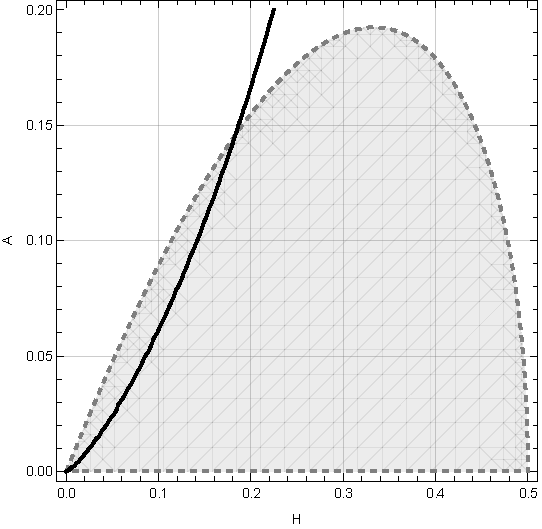
\includegraphics[width=.7\textwidth]{img/CurvaLyapunovAH.pdf}
	\caption{Curva $L_1 = 0$ y la región dada por las restricciones $H<1/2$ y $A^2 < H(1-2H)$.}
	\label{fig: curvaL_1AH}
\end{figure}

La curva $L_1 = 0$ y la región de restricciones del sistema, puede observarse en la \autoref{fig: curvaL_1AH}. El modelo contará con una bifurcación de Hopf subcrítica ($L_1 > 0$) para los valores de $A$ y $H$ que se encuentren por encima de esta curva y dentro de la región restrictiva, en este caso, $(H,H)$ es un foco débil estable rodeado por un ciclo límite inestable; de manera análoga el sistema poseerá una bifurcación de Hopf supercrítica para los valores que se encuentren debajo de esta curva y dentro de la región dada por las restricciones del sistema, aquí, $(H,H)$ es un foco débil inestable rodeado por un único ciclo límite estable. El caso $L_1 > 0$, es de vital importancia debido a las características del sistema, como la región $\Gamma$ es invariante, y los demás puntos críticos no poseen propiedades atractoras dentro de la región, las trayectorias fuera del ciclo límite inestable deben tender a otro ciclo limite estable según el teorema de Poincaré-Bendixson, esto garantiza la existencia de un ciclo límite adicional en este caso.

\begin{remark}
	Otro método para calcular el primer número de lyapunov es trasladar el sistema de estudio a la forma
	\begin{equation*}
		\begin{cases}
			\dot{X} = -\omega Y + \tilde{G}_1(X, Y), \\
			\dot{Y} = \omega X + \tilde{G}_2(X, Y),
		\end{cases}
		\label{eq: normalFormWn}
	\end{equation*}
	donde $\pm \omega i$ son los valores propios de la matriz jacobiana en el origen y \linebreak $\tilde{G}=(\tilde{G}_1,\tilde{G}_2)$ contiene los términos no lineales del sistema. El primer coeficiente de Lyapunov podrá ser determinado a partir de las derivadas parciales de $\tilde{G}$ evaluadas en 0 \cite[p. 152]{guckenheimer1983}: 
	\begin{equation*}
		\begin{aligned}
			16\tilde{l_1} &= \tilde{G}_{1,xxx} + \tilde{G}_{1,xyy} + \tilde{G}_{2,xxy} + \tilde{G}_{2,yyy} \\
			&+ \frac{1}{\omega} [ \tilde{G}_{1,xy}(\tilde{G}_{1,xx} + \tilde{G}_{1,yy}) - \tilde{G}_{2,xy}(\tilde{G}_{2,xx} + \tilde{G}_{2,yy}) \\
			&- \tilde{G}_{1,xx}\tilde{G}_{2,xx} + \tilde{G}_{1,yy}\tilde{G}_{2,yy} ].
		\end{aligned}
	\end{equation*}
	Siguiendo esta metodología, para el sistema \eqref{eq: modelo2Hen0} obtenemos que
	\begin{equation*}
		\tilde{l_1} = \dfrac{A^2 H(1 - H)([4 - 3H(3 - H)]A^4 -4H^3A^2 - (3 - H)H^5)}{2(A^2 + H^2)(H^3 + A^2(2 - H))(H^2(1 - 2H)- A^2)}.
		\label{eq: l1Perko}
	\end{equation*}
	Al igual que en el primer método empleado el signo de este valor depende de la expresión \eqref{eq: sgnL1}. Las diferencias en $l_1$ y $\tilde{l_1}$, se deben principalmente a la metodología impuesta para obtener este coeficiente, más sin embargo, no altera las conclusiones obtenidas. 
\end{remark}

Ahora, nótese que para el valor paramétrico $A=A_c$, el primer coeficiente de lyapunov se anula, teniendo como consecuencia no poder definir la estabilidad del punto de equilibrio $(H, H)$, en este caso. Para poder determinarla, debemos proceder a calcular el segundo coeficiente de lyapunov.

\begin{figure}
	\centering
	\begin{subfigure}{0.49\textwidth}
		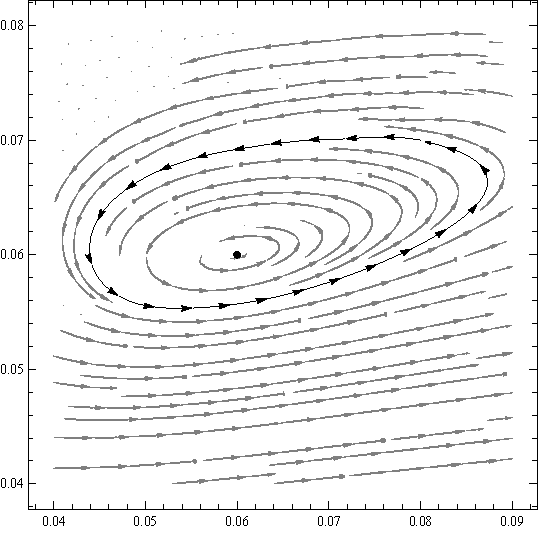
\includegraphics[width=\textwidth]{img/HopfSubCentrolineal.pdf}
		\caption{Bifurcación de Hopf subcrítica \linebreak ($l_1 = 0.0589$) del sistema \eqref{eq: modelo2} para los valores $A = 0.05; \; H = 0.06; \; B=B_c=0.109508$ y $Q=1.59278$ con el punto crítico de estudio como un foco débil estable.}
		\label{fig: bifurcacionHopfsub}
	\end{subfigure}
	\hfill
	\begin{subfigure}{0.49\textwidth}
		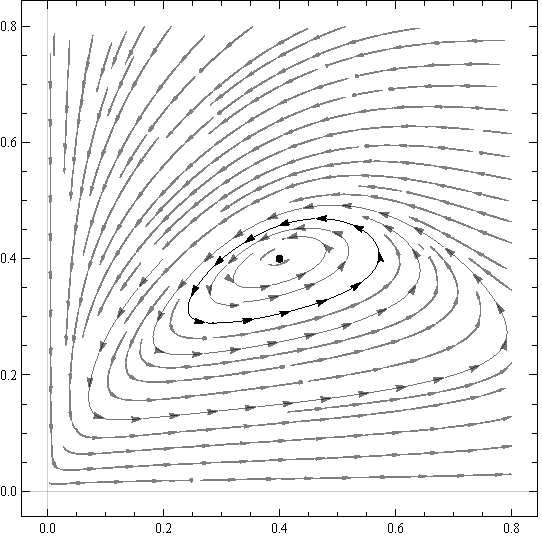
\includegraphics[width=\textwidth]{img/HopfSuperCentrolineal.pdf}
		\caption{Bifurcación de Hopf supercrítica ($l_1 = -0.0250864$) del sistema \eqref{eq: modelo2} para los valores $A = 0.05; \; H = 0.4; \; B=B_c=0.181538$ y $Q=0.609375$ con el punto crítico de estudio como un foco débil inestable.}
		\label{fig: bifurcacionHopfsup}
	\end{subfigure}
	\caption{Bifurcación de Hopf del sistema \eqref{eq: modelo2}.}
	\label{fig: bifurcacionHopf}
\end{figure}

%Esto además nos permitirá determinar que tipo de bifurcación de Bautin se nos presenta.
%
%\begin{teo}
%	Una bifurcación de Bautín (Hopf generalizada) ocurre en el equilibrio $(H, H)$ para los valores de bifurcación $\mu_0 = (A_c, B_c)$.
%\end{teo}
%\begin{proof}
%	Este hecho se da simplemente del caso de que el sistema posee valores propios complejos puros para $B=B_c$, y de que $L_1 = 0$ para $A = A_c$.
%\end{proof}

\subsubsection{Calculo del segundo coeficiente de Lyapunov}
Procedemos a reemplazar el valor paramétrico $A=A_c$ en el sistema \eqref{eq: formaBifHopf} con el fin de que $l_1 = 0$:
\begin{equation}
	Z_{\eta}:
	\begin{cases}
		\dfrac{d\bar{u}}{d \tau} = a\bar{u} + b\bar{v} + F_1(\bar{u}, \bar{v}),\\
		\dfrac{d\bar{v}}{d \tau} = a\bar{u} - a\bar{v} + F_2(\bar{u}, \bar{v}),
	\end{cases}
	\label{eq: normalFormZn}
\end{equation}
con $F=(F_{1}, F_2)$ dadas por las expansiones \eqref{eq: expansionF1,2}, sustituyendo $A=A_c$. La matriz jacobiana del sistema \eqref{eq: normalFormZn} en el origen estaría dada simplemente por la matriz \eqref{eq:jacobianamodelo2Hen0} realizando la sustitución correspondiente:
\begin{equation}
	Dh(0,0) =
	\begin{bmatrix}
		a & b \\
		a & - a
	\end{bmatrix},
\end{equation}
donde
\begin{equation*}
	\begin{aligned}
		a &= \frac{H^3(1 - H)[4 - 3H(5 - 2H) - \sqrt{3H(4 - H)}]}{4 - 3H(3 - H)}, \\
		b &= -\frac{H^3(1 - H)^2[4 - 3H + \sqrt{3H(4 - H)}]}{4 - 3H(3 - H)},
	\end{aligned}
\end{equation*}
bajo la restricción $0 < H < (3 - \sqrt{6})/3 \approx 0.1835$ que serían los valores para las cuales se satisfacen las restricciones $H<1/2$, $A^2 < H^2(1-2H)$ planteadas en la \autoref{sec: HH} al sustituir $A = A_c$.

El segundo coeficiente de Lyapunov está dado por
\begin{equation}
	\begin{aligned}
		12l_2 = {} & \frac{1}{\omega} \text{Re } g_{32} \\
		& + \frac{1}{\omega^2} \text{Im } \left[ g_{20} \bar{g}_{31} - g_{11} (4 g_{31} + 3 \bar{g}_{22}) - \frac{1}{3} g_{02} (g_{40} + \bar{g}_{13}) - g_{30} g_{12} \right] \\
		& + \frac{1}{\omega^3} \left\{ \text{Re } \left[ g_{20} \left( \bar{g}_{11} (3 g_{12} - \bar{g}_{30}) + g_{02} \left( \bar{g}_{12} - \frac{1}{3} g_{30} \right) + \frac{1}{3} \bar{g}_{02} g_{03} \right) \right.\right. \\
		& \qquad\qquad\qquad \left. + g_{11} \left( \bar{g}_{02} \left( \frac{5}{3} \bar{g}_{30} + 3 g_{12} \right) + \frac{1}{3} g_{02} \bar{g}_{03} - 4 g_{11} g_{30} \right) \right] \\
		& \qquad\qquad \left. + \, 3 \text{ Im}(g_{20} g_{11}) \text{ Im } g_{21} \right\} \\
		& + \frac{1}{\omega^4} \left\{ \text{Im} \left[ g_{11} \bar{g}_{02} \left( \bar{g}_{20}^2 - 3 \bar{g}_{20} g_{11} - 4 g_{11}^2 \right) \right] \right. \\
		& \qquad\qquad \left. + \, \text{Im}(g_{20} g_{11}) \left[ 3 \text{ Re}(g_{20} g_{11}) - 2 |g_{02}|^2 \right] \right\},
	\end{aligned}
	\label{eq: l2}
\end{equation}
con $\omega = \sqrt{ad}$, donde $$d = H^4+\frac{H^3(2-H) [2H+(1-H) \sqrt{3H(4-H)}]}{4-3H(3-H)}$$ y las expresiones $g_{kl}$ se determinan a partir del sistema \eqref{eq: sistemal1} transformado a la forma normal de Poincaré:
\begin{equation}
	\dot{z} = \omega i z + \sum_{2 \le k+l \le 5} \frac{1}{k!l!} g_{kl} z^k \bar{z}^l + O(|z|^6).
	\label{eq: normalForml2}
\end{equation}
O de igual manera, considerando las derivadas parciales de la función de variable compleja \eqref{eq: funComplejaL1},
con $p=(p_1,p_2)$ y $q=(q_1,q_2)$ dadas por \eqref{eq: vecComplejos}, donde $$m = \sqrt{\frac{d}{a}} = \sqrt{\frac{H(7-3H)+(1-H)\sqrt{3H(4-H)}}{2-6H(2-H)}}.$$ Las expresiones necesarias para el cálculo del segundo coeficiente de Lyapunov \eqref{eq: l2}, estarán dadas por los términos $g_{kl}=G_{z w}$ que representan las derivadas parciales de G evaluadas en $z=w=0$, donde por ejemplo \linebreak $g_{02}=G_{ww}, \; g_{31}=G_{zzzw}$, de manera similar se determinan las demás expresiones \cite[p. 344]{Kuznetsov2023}. Los términos $g_{20}, \; g_{11}, \; \text{y } g_{21}$ se determinan de \eqref{eq: g_klModelo2} remplazando $A=A_c$, además
\begin{equation}
	\begin{aligned}
		g_{31} = & \frac{i}{m} \{6(m^2+1)[-2 + (B_c-4)mi + (B_c+2)m^2 \\
		& - 10H(m-i)^2] - 6Q(m^3 + 3m -2i)\}, \\
		g_{32} = & \frac{-60}{m}(m-i)^3 (m+i)^2, \\
		g_{22} = & \frac{2i}{m} [4B_cm^2(1 - mi) + 6(5H-1)(m^2+1)^2 + 6Q(m^2+1)], \\
		g_{02} = & \frac{-(m+i)}{m}\{ A_c^2[1 - 3H + (B_c + 3H - 1)mi] \\
		& + H^2[6 + 2B_cm^2 + 10Hi(m+i) - 6Q + 3mi(B_c + Q - 2)] \}, \\
		g_{40} = & \frac{12i}{m} \{ 5H(m-i)^4 - (m-i)^2[-1 + (B_c+1)m^2 \\
		& + Q + (B_c + Q - 2)mi] \}, \\
		g_{13} = & \frac{-6i}{m} (m+i)^2[-2 + 10H - B_cmi \\
		& + m^2(B_c + 10H-2) + Q(mi+2)],
	\end{aligned}
\end{equation}
\begin{equation*}
	\begin{aligned}
		g_{30} = & \frac{3}{m} \{ [A_c^2 + 2H(5H-2)](m-i)^3 \\
		& + B_cHm(1 - mi)[m(m-4i)-3] + HQ(m-i)^2(m-4i) \}, \\
		g_{12} = & \frac{m+i}{m} \{3A_c^2(m^2+1) + H[30H(m^2+1)\\
		& + m[B_c(-3i + m(4 - 3mi)) + 3m(Q-4) + 3Qi] + 12(Q-1)]\}, \\
		g_{03} = & \frac{-3(m+i)^2}{m} \{A_c^2(m+i) \\
		& + H\left[10H(m+i) + 4i(Q-1) + m(B_c(3 - mi) + Q -4)\right]\},
	\end{aligned}
\end{equation*}
donde
\begin{equation*}
	\begin{aligned}
		B_c &= \frac{2-3H - \sqrt{3H(4 - H)}}{2}, \\
		Q &= H^2 \frac{H[2-3(3-H)]+(1-H)\sqrt{3H(4-H)}+4}{4-3H(3-H)}.
	\end{aligned}
\end{equation*}
Tomando en cuenta estas expresiones computamos $l_2$, para el cual se obtienen algunos valores como los mostrados en la siguiente tabla.
\begin{table}[H]
	\centering
	\caption{Valores de $l_2$ para parámetros aleatorios}
	\label{tab:ejemplosL2}
	
	\begin{tabular}{ccccl}
		\hline
		$H$ & $A$ & $B$ & $Q$ & $l_2$ \\
		\hline
		0.0247 & 0.0096 & 0.6918 & 1.1246 & -1021240 \\
		0.0645 & 0.0338 & 0.4671 & 1.1932 & -100399 \\
		0.0646 & 0.0339 & 0.4664 & 1.1933 & -100023 \\
		0.0900 & 0.0530 & 0.3511 & 1.2257 & -63026.4 \\
		0.0922 & 0.0548 & 0.3418 & 1.2283 & -61890.6 \\
		0.0953 & 0.0573 & 0.3289 & 1.2319 & -60651.6 \\
		0.1529 & 0.1114 & 0.1065 & 1.2971 & -180304 \\
		0.1633 & 0.1227 & 0.0694 & 1.3091 & -409538 \\
		0.1717 & 0.1321 & 0.0404 & 1.3190 & -1314910 \\
		0.1720 & 0.1325 & 0.0392 & 1.3194 & -1402770 \\
		\hline
	\end{tabular}
\end{table}

\noindent Teniendo en cuenta los datos obtenidos en la \autoref{tab:ejemplosL2}, graficamos $-l_2$ en escala logarítmica (ver \autoref{fig: curvaL_2H}), el cual será estrictamente positivo, es decir, tendríamos que para cualquier valor $H \in \left(0,(3 - \sqrt{6})/3 \right)$, $l_2<0$; por lo tanto, el punto crítico $(H,H)$ es un foco débil estable de segundo orden \cite[p. 518]{chicone2024}, rodeado por un ciclo límite inestable y este a su vez, por un ciclo límite estable.

\begin{figure}[H]
	\centering
	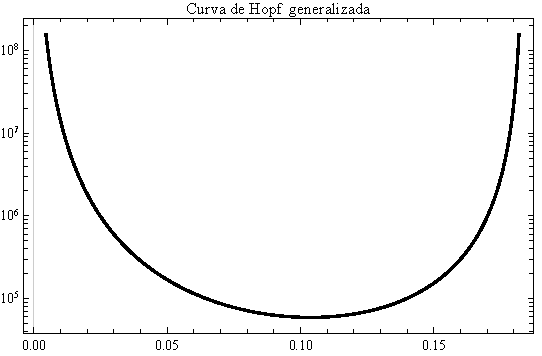
\includegraphics[width=.6\textwidth]{img/CurvaLyapunov2H.pdf}
	\caption{Curva $-l_2$ en escala logarítmica, dentro del dominio biológicamente relevante $0 < H < (3 - \sqrt{6})/3$.}
	\label{fig: curvaL_2H}
\end{figure}

\noindent Ya que $l_2$ es siempre negativo, obtenemos el siguiente teorema.

\begin{teo}
	Una bifurcación de Hopf generalizada (Bautin) ocurre en el equilibrio $(H, H)$ para el valor de bifurcación $\mu_0=(A_c, B_c)$.
\end{teo}
\begin{proof}
	Es claro que para $A= A_c$, $l_1 = 0$; así, para que ocurra una bifurcación de Bautín se deben satisfacer la condición espectral y la de transversalidad. Por el \Cref{teo:Hopf} la condición espectral se cumple. Por otra parte, el mapeo $\mu = (A,B) \longmapsto \left(Re(\lambda(\mu)), l_1(\mu)\right)$ debe ser regular en $\mu=\mu_0$, es decir
	\begin{equation*}
		\det \left. \begin{pmatrix}
			\frac{\partial Re(\lambda(\mu))}{\partial A} & \frac{\partial Re(\lambda(\mu))}{\partial B} \\[6pt]
			\frac{\partial l_1(\mu)}{\partial A} & \frac{\partial l_1(\mu)}{\partial B} 
		\end{pmatrix} \right|_{\mu=\mu_0} \neq 0,
	\end{equation*}
	esto es
	\begin{equation}
		\left. - \frac{\partial Re(\lambda(\mu))}{\partial B} \left( \frac{\partial l_1(\mu)}{\partial A} - \frac{\frac{\partial Re(\lambda(\mu))}{\partial A}}{\frac{\partial Re(\lambda(\mu))}{\partial B}} \frac{\partial l_1(\mu)}{\partial B} \right) \right|_{\mu=\mu_0} \neq 0.
		\label{eq: regularidadBautin}
	\end{equation}
	Como $Re(\lambda(\mu_0))=0$ y del \Cref{teo:Hopf} sabemos que \linebreak $\left. \frac{\partial Re(\lambda(\mu))}{\partial B} \right|_{\mu=\mu_0} \neq 0$, por el teorema de la función implícita existe una función diferenciable $\phi(A)=B$ con dominio en una vecindad $V$ de $A_c$ tal que
	\begin{equation}
		\frac{dB}{dA}=\phi'(A)= - \frac{\frac{\partial Re(\lambda(\mu))}{\partial A}}{\frac{\partial Re(\lambda(\mu))}{\partial B}}, \; A \in V.
		\label{eq: teoFunImpli}
	\end{equation}
	Considerando lo anterior, por la regla de la cadena $$\frac{d l_1(A, \phi(A))}{dA} = \frac{\partial l_1(A, \phi(A))}{\partial A} + \phi'(A) \frac{\partial l_1(A, \phi(A))}{\partial \phi(A)},$$ así por lo anterior y por \eqref{eq: teoFunImpli} para una vecindad $V$ de $A_c$ la regularidad \eqref{eq: regularidadBautin} se reduce a probar que $$\left. \frac{d l_1(A, \phi(A))}{dA} \right|_{A=A_c} \neq 0.$$ Ahora, nótese que la función $\phi(A)$ está dada simplemente por $B_c(A)$ obtenida en \eqref{eq: Bcritico}, por lo que basta mostrar que la derivada con respecto a $A$ de $l_1$ determinada en \eqref{eq: l1Kuznetsov}, no se anula para $A=A_c$. Con este objetivo, considerando
	\begin{equation*}
		\begin{aligned}
			N &= 2A^2(1 - H)([4 - 3H(3 - H)]A^4 -4H^3A^2 - (3 - H)H^5) ,\\
			I &= (H^3 + A^2(2 - H))(H^2(1 - 2H)- A^2),
		\end{aligned}
	\end{equation*}
	de \eqref{eq: l1Kuznetsov} tenemos que $$l_1 = \frac{N}{(A^2+H^2)I^{3/2}},$$ asi
	\begin{equation}
		\frac{dl_1}{dA} = \frac{N' (A^2+H^2) I^{3/2} - N \left[2AI^{3/2} + (3/2)(A^2+H^2) I^{1/2} I' \right]}{(A^2+H^2)^2 I^3},
	\end{equation}
	por las restricciones del sistema $(A^2+H^2) I^{3/2} > 0$ y como $N=0$ en $A=A_c$ tenemos que $\left. \frac{d l_1}{dA} \right|_{A=A_c} \neq 0$ si, y solo si $N' \neq 0$ para $A=A_c$. Ahora el signo de
	\begin{equation*}
		N'= 4A(1-H) \left(3[4-3H(3-H)]A^4-8H^3A^2-(3-H)H^5\right)
	\end{equation*}
	estará determinado por la expresión $$3[4-3H(3-H)]A^4-8H^3A^2-(3-H)H^5,$$ la cual se anulará para
	\begin{equation*}
		\begin{aligned}
			A^2 &= \dfrac{8H^3 \pm \sqrt{64 H^6 + 12[4 - 3H(3-H)] (3-H)H^5}}{6[4-3H(3-H)]} \\
			&= \frac{1}{3} \dfrac{4H^3 + H^2\sqrt{36H - H^2[77 - 9H(6 - H)]}}{4-3H(3-H)} \neq A^2_c.
		\end{aligned}
	\end{equation*}
	Cumpliéndose así la condiciones necesarias para la bifurcación de Hopf generalizada en $\mu=\mu_0$.
\end{proof}

\begin{figure}[H]
	\centering
	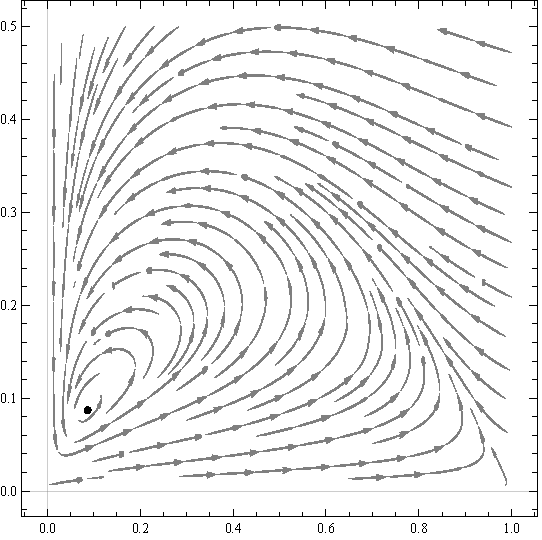
\includegraphics[width=.6\textwidth]{img/HopfGeneralCentrolineal.pdf}
	\caption{Bifurcación de Hopf generalizada ($l_2 = -65014.612$) del sistema \eqref{eq: modelo2} para los valores $H = 0.086966; \; A = A_c = 0.050591; \; B=B_c=0.36435$ y $Q=1.22202$ con el punto crítico de estudio como un foco débil estable de segundo orden.}
	\label{fig: bifurcacionHopfGeneral}
\end{figure}
	%\chapter{Conclusiones}
%En este trabajo se realizó un análisis cualitativo y local de un modelo depredador-presa con respuesta funcional Holling tipo 3, propuesto originalmente por Gonzáles-Olivares, et al., 2015 \cite{articulo}. Tras un cambio de variables y un reescalado temporal con el fin de facilitar el análsis se logro obtener un sistema topologicamente equivalente, que este a su vez permitio analizar el origen algo que el sistema original no permitia estudiar, tras un detallado estudio de este nuevo sistema polinomial de 5to orden de ecuaciones diferenciales ordinarias, se obtuvieron los siguientes resultados:
%
%\begin{enumerate}
%	\item Se determinó que el cuadrado unitario $$\Gamma = \{ (u, v) \in \R^{2} \; | \; 0 \leq u \leq 1, \; 0 \leq v \leq 1 \} \subset \tilde{\Omega},$$ es una región positivamente invariante, concluyendo así que las soluciones son acotadas dentro de esta región.
%	\item Se obtivieron tres puntos de equilibrio biológicamente relevantes: \linebreak $(0,0), \; (1,0) \; \text{y} \; (H,H)$ con $H \in (0,1)$ determinado por la interseccion de las isoclinas \eqref{eq:isoclina-presa_modelo2} y $u=v$.
%	\item Se clasificó el punto de equilibrio $(1,0)$ como un punto silla sin importar el valor de los parámetros del sistema.
%	\item Se demostró que el punto de equilibrio $(0,0)$ se comporta localmente como una silla sin importar los valores paramétricos, tras haber determinado el índice de Poincaré realizando un análisis sectorial a través de la técnica del explotado polar (Blowing-up), en el cual se halló que si el parámetro $B$ es mayor o igual que 1, el primer cuadrante constará de una separatriz determinada por la pendiente $\tan \theta_3 = \dfrac{B-1}{B}$, la cual divide el retrato fase en dos sectores distintos: hiperbólico y parabólico; por otra parte, si $B<1$ el primer cuadrante estará dado por un único sector hiperbólico.  
%	\item Se halló que la estabilidad del punto de equilibrio $(H,H)$ está fuertemente relacionada con los valores paramétricos, obteniendo la siguiente clasificación:
%	\begin{itemize}
%		\item Si $B<B_c$ y
%		\subitem $\Delta < 0$, $(H,H)$ es un foco inestable.
%		\subitem $\Delta = 0$, $(H,H)$ es un nodo degenerado inestable.
%		\subitem $\Delta > 0$, $(H,H)$ es un nodo inestable.
%		\item Si $B=B_c$ y
%		\subitem $A < A_c$, ocurre una bifurcación de Hopf supercrítica por lo que $(H,H)$ es un foco débil inestable rodeado de un ciclo límite estable.
%		\subitem $A = A_c$, ocurre una bifurcación de Bautin supercrítica ($l_2<0$), por lo que $(H,H)$ es un foco débil estable de segundo orden rodeado por un pequeño ciclo límite inestable que a su vez esta dentro de un segundo ciclo limite estable.
%		\subitem $A > A_c$, ocurre una bifurcación de Hopf subcrítica por lo que $(H,H)$ es un foco débil estable rodeado de un ciclo límite inestable.
%		\item Si $B>B_c$ y
%		\subitem $\Delta < 0$, $(H,H)$ es un foco estable.
%		\subitem $\Delta = 0$, $(H,H)$ es un nodo degenerado estable.
%		\subitem $\Delta > 0$, $(H,H)$ es un nodo estable.
%	\end{itemize}
%\end{enumerate}
%
%\chapter{Discusión y trabajos a futuro}
%El difeomorfismo aplicado para la equivalencia topologia entre el sistema original y el sistema polinomial \eqref{eq:modelo1}, garantiza que el estudio biologicamente relevante para el modelo polinomial \eqref{eq: modelo2} se encuentra dentro de la región $\Gamma$, debido a la ``normalización" hecha en las sustituciones $u = x/K$ y $v = y / n K $ impuesta por las capacidades de carga tanto de la presa como el depredador, haciendo irrelevante el estudio fuera del cuadrado unitario $\Gamma$.
%
%El caso $B<B_c$ donde el equilibrio $(H,H)$ es inestable, garantiza la existencia de un ciclo límite estable, debido a la region de atrapamiento $\Gamma$, a que los demas puntos criticos no poseen propiedades atractoras y al teorema de poincaré-bendixson, por tal misma razon se garantiza la existencia de un segundo ciclo límite estable para el caso de la bifurcacion de Hopf subcritica $B=B_c$ y $A>A_c$, en este caso donde hay dos ciclos limites y en el caso de la bifurcación de Bautin ($(A_c,B_c)$), es posible que ante la variación de los parámetros restantes se produzca una colision de ciclos limites dando como resultado en un ciclo limite semiestable, esto tambien es conocido como bifurcacion de ciclos limites y puede ser de estudio, mas informacion al respecto puede encontrarse en \cite[p. ~189]{Kuznetsov2023}.
%
%Para el caso $B>1$ es altamente probable que la orbita separatriz determinada por la pendiente $\tan \theta_3 = \dfrac{B-1}{B}$, tambien constituya una orbita heteroclinica entre $(0,0) \; \text{y} \; (H,H)$ debido a que estariamos en el caso $B>B_c$ donde el equilibrio $(H,H)$ es estable, bastaría mostrar que dicha separatiz en realidad pertenece a la variedad estable de $(H,H)$.
%
%La proyección a futuro de las densidades poblacionales, estará fuertemente arraigada a las condiciones iniciales y a los valores paramétricos, en general, la única posbilidad de que ambas especies logren extinguirse solo se da en el caso de que las condiciones iniciales se encuntre sobre el semieje positivo $u=0$, es decir ante la ausencia de presas, ahora ante la ausencia de depredadores, es decir, si las condiciones iniciales se encuentran dentro del semieje positivo $v=0$, las presas tenderan al equilibrio $(1,0)$, en otras palabras creceran hasta tal punto que el ambiente lo pueda soportar. En otro caso, si las condiciones iniciales estan fuera de los semiejes positivos las especies tenderan a una orbita periódica (ciclo límite) o al equilibrio $(H,H)$, donde esta última tendencia puede ser extremadamente lenta si el equilibrio es un foco debil estable o peor aún si es de segundo orden. En conclusión, bajo condiciones inciales factibles (fuera de los ejes) la preservación de las especies que se moldeen al sistema estudiado, está garantizada, revelando así la importancia de todo lo estudiado en el presente trabajo.

\chapter{Conclusiones}

En este trabajo se realizó un análisis cualitativo y local de un modelo depredador--presa tipo Leslie-Gower con respuesta funcional de Holling tipo III, propuesto originalmente por Gonzáles-Olivares et al.~\cite{articulo}. Mediante un cambio de variables y un reescalamiento temporal, realizado con el propósito de facilitar el análisis, se obtuvo un sistema topológicamente equivalente al modelo original. Esta transformación permitió, además, incorporar el origen al dominio de estudio y analizar su comportamiento local, aspecto que no era posible estudiar directamente en el sistema original.

A partir del estudio cualitativo del sistema polinomial de quinto orden obtenido, se establecieron los siguientes resultados:

\begin{enumerate}
	\item Se determinó que el cuadrado unitario
	\[
	\Gamma =
	\left\{
	(u,v)\in\mathbb{R}^{2} \; \middle| \;
	0\leq u\leq 1,\;
	0\leq v\leq 1
	\right\}
	\subset \tilde{\Omega},
	\]
	es una región positivamente invariante. En consecuencia, toda solución que inicia en $\Gamma$ permanece en esta región para todo tiempo futuro, por lo que las soluciones biológicamente relevantes son acotadas, lo que demuestra que el modelo Leslie-Gower modificado está bien planteado.
	
	\item Se obtuvieron tres puntos de equilibrio biológicamente relevantes:
	\[
	(0,0), \qquad (1,0), \qquad \text{y} \qquad (H,H),
	\]
	donde $H\in(0,1)$ está determinado por la intersección de las isoclinas
	\eqref{eq:isoclina-presa_modelo2} y $u=v$.
	
	\item Se clasificó el punto de equilibrio $(1,0)$ como un punto silla, independientemente de los valores de los parámetros del sistema.
	
	\item Se demostró que el punto de equilibrio $(0,0)$ se comporta localmente como un punto silla--nodo, independientemente de los valores de los parámetros. Para ello, se determinó su índice de Poincaré mediante un análisis sectorial basado en la técnica de \emph{blowing-up} (explotado polar).
	
	En particular, cuando $B\geq 1$, se encontró que el primer cuadrante contiene una separatriz cuya dirección está determinada por
	\[
	\tan\theta_3=\frac{B-1}{B}.
	\]
	Esta separatriz divide el retrato de fase local en dos sectores: uno hiperbólico y otro parabólico. Por otro lado, cuando $B<1$, el primer cuadrante está constituido localmente por un único sector hiperbólico.
	
	\item Se determinó que la estabilidad del punto de equilibrio $(H,H)$ depende de manera fundamental de los valores de los parámetros del sistema. En particular, se obtuvo la siguiente clasificación:
	
	\begin{itemize}
		\item Si $B<B_c$, entonces:
		\begin{itemize}
			\item si $\Delta<0$, el equilibrio $(H,H)$ es un foco inestable;
			\item si $\Delta=0$, $(H,H)$ es un nodo degenerado inestable;
			\item si $\Delta>0$, $(H,H)$ es un nodo inestable.
		\end{itemize}
		
		\item Si $B=B_c$, entonces:
		\begin{itemize}
			\item si $A<A_c$, ocurre una bifurcación de Hopf supercrítica, por lo que $(H,H)$ es un foco débil inestable rodeado por un ciclo límite estable;
			
			\item si $A=A_c$, ocurre una bifurcación de Bautin supercrítica, con $l_2<0$. En este caso, $(H,H)$ es un foco débil estable de segundo orden, rodeado por un ciclo límite pequeño e inestable, el cual se encuentra contenido en el interior de un segundo ciclo límite estable;
			
			\item si $A>A_c$, ocurre una bifurcación de Hopf subcrítica, por lo que $(H,H)$ es un foco débil estable rodeado por un ciclo límite inestable.
		\end{itemize}
		
		\item Si $B>B_c$, entonces:
		\begin{itemize}
			\item si $\Delta<0$, el equilibrio $(H,H)$ es un foco estable;
			\item si $\Delta=0$, $(H,H)$ es un nodo degenerado estable;
			\item si $\Delta>0$, $(H,H)$ es un nodo estable.
		\end{itemize}
	\end{itemize}
\end{enumerate}

En conjunto, estos resultados permiten caracterizar la dinámica local de los principales estados de equilibrio del modelo y establecer una relación entre la estabilidad del equilibrio de coexistencia $(H,H)$, la aparición de ciclos límite y la variación de los parámetros del sistema. Asimismo, el análisis realizado proporciona una descripción cualitativa de los posibles comportamientos asintóticos de las poblaciones dentro de la región biológicamente relevante.


\chapter{Discusión y trabajos a futuro}

El difeomorfismo empleado para establecer la equivalencia topológica entre el sistema original y el sistema polinomial \eqref{eq:modelo1} permite restringir el análisis biológicamente relevante del modelo transformado a la región $\Gamma$. En efecto, las sustituciones
\[
u=\frac{x}{K},
\qquad
v=\frac{y}{nK},
\]
normalizan las densidades poblacionales con respecto a las capacidades de carga asociadas a la presa y al depredador. De esta manera, los valores $u=1$ y $v=1$ representan, respectivamente, los niveles de población asociados a dichas capacidades de carga. Por tanto, el estudio de la dinámica dentro del cuadrado unitario $\Gamma$ resulta particularmente relevante desde el punto de vista biológico.\\

Uno de los principales resultados obtenidos está relacionado con la existencia de ciclos límite y su dependencia respecto de los parámetros del modelo. Cuando $B<B_c$, el equilibrio $(H,H)$ es inestable. Dado que $\Gamma$ es una región positivamente invariante y que los restantes puntos de equilibrio no presentan propiedades atractoras en el interior de la región, el teorema de Poincaré--Bendixson proporciona un mecanismo para establecer la existencia de una órbita periódica bajo las condiciones apropiadas; similarmente, es posible garantizar la existencia de un ciclo límite adicional en el caso donde ocurre una bifurcación de Hopf subcrítica. En particular, estos resultados son consistentes con la interpretación biológica de oscilaciones persistentes en las densidades de presa y depredador.

\begin{figure}[H]
	\centering
	\begin{subfigure}{0.49\textwidth}
		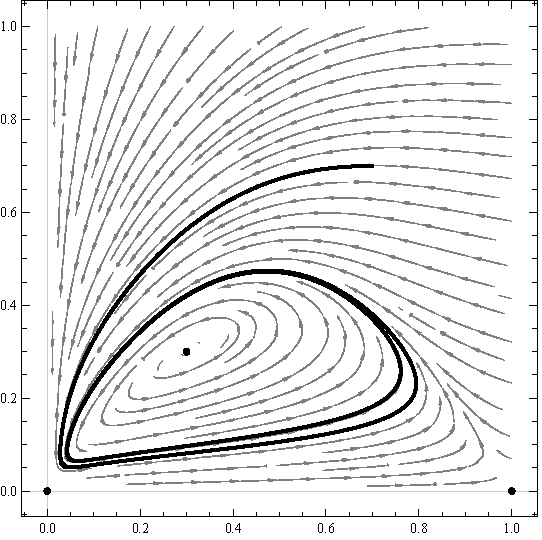
\includegraphics[width=\textwidth]{img/hFocoInestable.pdf}
		\caption{Retrato fase del sistema \eqref{eq: modelo2} para $A = 0.03; \; B = 0.3$ y $Q = 0.707$ con $(H,H)$ como foco inestable, rodeado por un ciclo límite estable.}
	\end{subfigure}
	\hfill
	\begin{subfigure}{0.49\textwidth}
		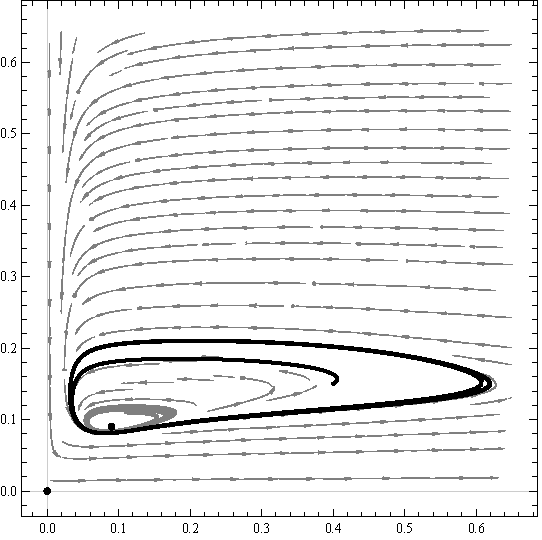
\includegraphics[width=\textwidth]{img/HopfSubCentrolinealVersion2.pdf}
		\caption{Bifurcación de Hopf subcrítica del sistema \eqref{eq: modelo2} para $A = 0.078; \; B = 0.0643$ y $Q = 1.594$ con $(H,H)$ como foco débil estable, rodeado por un ciclo límite inestable y este a su vez por una orbita periódica estable.}
	\end{subfigure}
	\caption{Orbitas periódicas del modelo de estudio.}
\end{figure}

Por otra parte, en el punto de Bautin $(A_c,B_c)$ se identificó la presencia de dos ciclos límite, uno estable y otro inestable. Esta configuración plantea la posibilidad de que, ante una variación adicional de los parámetros, ambos ciclos límite colisionen y den lugar a un ciclo límite semiestable. Este fenómeno corresponde a una bifurcación de ciclos límite y constituye una extensión natural del análisis realizado. Un estudio detallado de este tipo de bifurcaciones puede consultarse en \cite[p.~189]{Kuznetsov2023}.\\

Otro problema de interés surge para $B>1$. En este caso, el análisis local del origen permitió identificar una separatriz cuya dirección está determinada por
\[
\tan\theta_3=\frac{B-1}{B}.
\]
Es razonable plantear como hipótesis que esta órbita separatriz pueda constituir una conexión heteroclínica entre $(0,0)$ y $(H,H)$, particularmente debido a que para $B>B_c$ el equilibrio $(H,H)$ es estable. No obstante, esta afirmación requiere una demostración adicional. En particular, sería necesario establecer que la separatriz asociada al origen pertenece efectivamente a la variedad estable de $(H,H)$. La demostración de esta propiedad constituiría una extensión natural del análisis realizado y permitiría obtener una descripción global más completa del retrato de fase. \\

\begin{figure}[H]
	\centering
	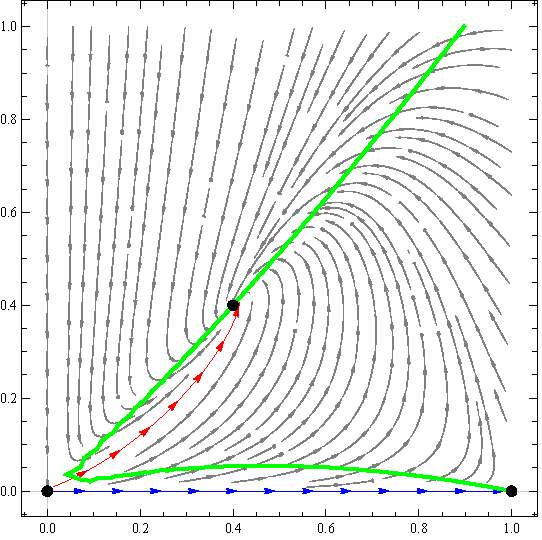
\includegraphics[width=.5\textwidth]{img/VariedadesInestablesOrigenBmayor1.pdf}
	\caption{Variedad inestable e isoclina asociada a la pendiente $\frac{B-1}{B}$ del sistema \eqref{eq: modelo2}, para $A = 0.05; \; B = 1.5$ y $Q = 0.61$.}
\end{figure}

Desde el punto de vista biológico, los resultados obtenidos muestran que la dinámica a largo plazo de las poblaciones depende tanto de las condiciones iniciales como de los valores de los parámetros. En particular, dentro de la región biológicamente relevante, la extinción simultánea de ambas especies únicamente puede ocurrir cuando las condiciones iniciales se encuentran sobre el semieje positivo $u=0$, correspondiente a la ausencia inicial de presas. Por otro lado, en ausencia de depredadores, es decir, cuando las condiciones iniciales pertenecen al semieje positivo $v=0$, la dinámica conduce al equilibrio $(1,0)$, que representa el crecimiento de la población de presas hasta el nivel determinado por la capacidad de carga del ambiente.

\noindent Cuando ambas poblaciones están inicialmente presentes, es decir, cuando las condiciones iniciales no se encuentren en los semiejes positivos $u=0$ y $v=0$, los resultados obtenidos indican que la dinámica puede conducir al equilibrio de coexistencia $(H,H)$ o a una órbita periódica, dependiendo de los valores de los parámetros y de las condiciones iniciales. Además, cuando $(H,H)$ es un foco débil estable, la convergencia hacia dicho equilibrio puede ser particularmente lenta. Este fenómeno es aún más pronunciado cuando el equilibrio corresponde a un foco débil de segundo orden, como ocurre en el punto de Bautin.

\noindent Los resultados anteriores permiten concluir que, para condiciones iniciales biológicamente factibles en las que ambas especies están presentes, el modelo estudiado no predice la extinción de ambas poblaciones. En su lugar, la dinámica conduce hacia un estado de coexistencia estacionario o hacia oscilaciones persistentes representadas por un ciclo límite. Esto resalta la importancia del análisis cualitativo realizado, pues permite identificar no solo los estados de equilibrio del sistema, sino también las estructuras dinámicas responsables de la persistencia o de las oscilaciones de las poblaciones.\\

El análisis realizado permite caracterizar los principales escenarios dinámicos del sistema y establecer su relación con los cambios de estabilidad de los puntos de equilibrio y con las bifurcaciones identificadas. En particular, los retratos de fase presentados en los capítulos anteriores permiten visualizar la presencia de una curva separatriz para el valor paramétrico estipulado; asimismo la aparición y estabilidad de los ciclos límite, incluyendo el ciclo límite estable que se observa cuando el equilibrio (H,H) pierde su estabilidad, así como el comportamiento asociado a la bifurcación de Hopf subcrítica. Estos resultados numéricos complementan el análisis cualitativo y permiten ilustrar de manera directa los distintos regímenes dinámicos identificados.\\

Como trabajos a futuro, se propone profundizar en el análisis del sistema. En particular, resulta de interés demostrar o refutar la existencia de la conexión heteroclínica asociada a la separatriz del origen y estudiar rigurosamente las posibles bifurcaciones de ciclos límite alrededor del punto de Bautin. Este análisis permitiría profundizar en la descripción de la dinámica más allá de los resultados locales asociados a los puntos de equilibrio y las bifurcaciones.
	\nocite{*}
	\bibliography{referencias}
\end{document}